% !Mode:: "TeX:UTF-8"
%!TEX program = xelatex
\documentclass[bwprint]{gmcmthesis}

% !Mode:: "TeX:UTF-8"

% 每个一级标题另起一页、居中
\usepackage{titlesec}
\titleformat{\section}{\clearpage\normalfont\Large\bfseries\centering}{\thesection}{1em}{}

% 公式、图、表按章节编号
\numberwithin{equation}{section}
\numberwithin{figure}{section}
\numberwithin{table}{section}

\usepackage{enumitem}
\setlist[enumerate,1]{label=(\arabic*),leftmargin=2.2em,itemsep=2pt,topsep=3pt}
\setlist[enumerate,2]{label=(\alph*)}
\setlist[itemize]{itemsep=2pt,topsep=3pt}

\usepackage{amsmath}
\usepackage{longtable}
\usepackage{booktabs}
\usepackage{array}
\usepackage{ragged2e}
\usepackage{float}
\usepackage{subfig}
\usepackage{colortbl}
\usepackage{threeparttable}

% 与插图统一的配色（见 论文图片/paper_style.py）
\definecolor{pblue}{HTML}{2F5D8A}
\definecolor{porange}{HTML}{D98A3A}
\definecolor{pgreen}{HTML}{4E9A78}
\definecolor{pred}{HTML}{C0504D}
\definecolor{pgray}{HTML}{8C8C8C}
\definecolor{thead}{HTML}{E4ECF4}   % 表头浅蓝
\definecolor{trow}{HTML}{F4F7FB}    % 隔行浅底
\definecolor{color1}{rgb}{0.78,0.88,0.99}
\definecolor{color2}{rgb}{0.36,0.62,0.84}
\definecolor{color3}{rgb}{0.88,0.92,0.96}
\definecolor{color4}{rgb}{0.96,0.97,0.98}

% 图表标题：小五号，标签加粗
\captionsetup{font=small,labelfont=bf,skip=4pt}
\setlength{\abovecaptionskip}{4pt}
\setlength{\belowcaptionskip}{0pt}
\setlength{\textfloatsep}{10pt plus 2pt minus 2pt}
\setlength{\floatsep}{8pt plus 2pt minus 2pt}
\setlength{\intextsep}{8pt plus 2pt minus 2pt}
\renewcommand{\arraystretch}{1.15}

% 定理类环境按章编号
\counterwithin{definition}{section}
\counterwithin{theorem}{section}
\counterwithin{corollary}{section}
\counterwithin{assumption}{section}

% 目录只到二级标题
\setcounter{tocdepth}{2}

% 结论框：用于每问末尾的“本问主要结论”
\usepackage[framemethod=TikZ]{mdframed}
\usetikzlibrary{arrows.meta,positioning}
\newmdenv[linecolor=pblue,linewidth=0.8pt,backgroundcolor=trow,roundcorner=3pt,
  innertopmargin=6pt,innerbottommargin=6pt,innerleftmargin=8pt,innerrightmargin=8pt,
  skipabove=8pt,skipbelow=6pt]{conclusionbox}

% 算法
\usepackage[noend]{algpseudocode}
\usepackage{algorithmicx,algorithm}
\floatname{algorithm}{算法}
\renewcommand{\algorithmicrequire}{\textbf{输入:}}
\renewcommand{\algorithmicensure}{\textbf{输出:}}

% listings 默认样式所需颜色
\definecolor{dkgreen}{rgb}{0,0.5,0}
\definecolor{mauve}{rgb}{0.58,0,0.82}
\definecolor{gray}{rgb}{0.5,0.5,0.5}
\usepackage{url}
\makeatletter\g@addto@macro{\UrlBreaks}{\do\_\do-}\makeatother

\newcommand{\red}[1]{\textcolor{red}{#1}}
\newcommand{\blue}[1]{\textcolor{blue}{#1}}
\newcommand{\todo}[1]{\textcolor{red}{\textbf{【待补：#1】}}}

\title{算力约束下提升大语言模型能力的资源配置建模}
\baominghao{20260079591} %参赛队号
\schoolname{华侨大学}%学校名称
\membera{梅芷涵} %队员A
\memberb{罗加印} %队员B
\memberc{刘玫均} %队员C


\begin{document}

\maketitle

\begin{abstract}

面向算力增长放缓与高质量语料稀缺的双重约束，大语言模型训练需要同时协调参数规模、训练数据量、数据质量、领域配比和长上下文开销。本文建立“数据属性建模——广义标度律——算力约束优化——能力前沿预测”的分层框架，对不同来源数据采用拟合、验证、压力测试和外推分层处理，并仅在通过物理与数值验收后向后续问题传递冻结接口。

针对问题一，将 $22$ 项异构质量信号同向化后划分为五个语义块，利用稳定 CRITIC 权重与冲突自适应 Huber 聚合得到样本和领域质量；在单纯形上建立二阶 Scheff\'e--Ridge 多输出响应面，并在经验支持域内进行多起点近优配比搜索。质量聚合方案扰动下七域排序的最低 Kendall 系数为 $0.8095$；二阶 Ridge 内部 NRMSE 为 $0.3959$，在 $1\mathrm{M}$、$60\mathrm{M}$ 和 $1\mathrm{B}$ 实测检验上的 Spearman 系数分别为 $0.8582$、$0.8698$ 和 $0.8503$。近优解对正则强度较稳健，但对支持半径和领域份额上界敏感，因而将其报告为近优配比族而非唯一全局最优解。

针对问题二，先比较参数--数据可分幂律、总算力幂律和交互幂律，再用分块留出验证选择质量修正形式，建立固定参考配比的广义标度律。参数--数据可分模型的留一规模 RMSE 为 $0.000147$，GQ2 质量修正模型在 $69$ 个留出块上的等权 RMSE 为 $0.072$。在中位参考点上，质量提高 $0.10$ 的 Loss 改善约等价于参数量增加 $37.30\%$ 或训练数据量增加 $56.95\%$。由于 A、B 体系缺少配比绝对效应的共同校准，非零配比强度在部分情景中还会跌破不可约损失，故联合配比接口不进入主决策。

针对问题三，固定参考领域配比，将基础训练、质量提升和长上下文注意力开销纳入同一 FLOPs 预算，联合优化 $N$、$D$ 和 $Q_A$。利用 Loss 对 $D$ 严格递减的结构解析消去 $D$，结合粗网格、多起点局部精化、三维独立复核与 KKT 边际条件识别资源结构转移。注意力开销与基础训练开销相当的上下文临界长度为 $30000$ Token。在 $4096$ 上下文、指数质量成本和 $10^{22}$ FLOPs 下，最优配置为 $N^*=5.44886\mathrm{B}$、$D^*=244.275\mathrm{B}$、$Q_A^*=0.999999$，预测 Loss 为 $2.15491$。连续预算路径呈现“质量未启动——质量与规模竞争——质量饱和后规模重新主导”的阶段变化，高预算结果则需保留外推标记。

针对问题四，以六项 Benchmark 重建综合能力，通过单调 Loss--Benchmark 桥接将问题三的 $45$ 个冻结情景映射到能力尺度，再以条件分位动力学模型和 Shapley 路径平均分解历史前沿。$2024$ 年 $6$ 月至 $2025$ 年 $1$ 月的能力增量为 $4.6182$ 分，其中规模扩张相关贡献为 $4.6183$ 分，控制规模后的非规模残余区间跨零，尚无稳定方向。若近期算力对数增速分别保留 $100\%$、$50\%$ 和 $25\%$，则 $24$ 个月后 $0.90$ 能力前沿中心值约为 $77.15$、$65.74$ 和 $59.16$。上述结果均是给定数据截止日、支持域和成本情景下的条件结论。

\noindent \textbf{关键词：}大语言模型\quad 数据质量\quad 广义标度律\quad 算力约束\quad 资源配置\quad 能力前沿

\end{abstract}


\pagestyle{plain}

\tableofcontents

\section{问题重述}

\subsection{问题背景}

近年来，大语言模型（Large Language Models，LLMs）在知识问答、代码生成和复杂推理等任务中表现出显著的规模效应。经典标度律表明，验证损失通常随模型参数量和训练 Token 数增加而下降，这为估计不同训练规模下的模型性能提供了经验基础。然而，参数量和数据量只描述了训练资源的数量维度：相同规模的训练数据可能具有不同质量，不同领域的组合方式也会改变模型在各类验证任务上的表现。此外，预训练 Loss 与下游 Benchmark 能力虽具有相关性，却并非可以直接互换的同一指标。

在实际训练中，算力和高质量语料均是有限资源。增大参数量和训练数据量会直接提高基础训练成本，数据清洗、筛选与重构会产生额外的质量提升成本，而长上下文训练还会引入随上下文窗口增长的注意力开销。领域配比虽然不必然增加 Token 总量，却决定有限数据预算在不同知识领域之间的分配。因此，模型性能提升实质上是参数规模、数据规模、数据质量、领域配比和上下文需求共同作用下的多资源配置问题。

基于此，本文围绕“数据属性刻画--广义损失建模--算力约束优化--能力前沿预测”展开研究：首先建立样本与领域质量评价体系并识别领域配比效应；其次将质量和配比因素引入经典标度律；随后在统一算力预算下求解参数、数据与质量投入的条件最优配置；最后连接预训练 Loss 与下游 Benchmark，分析历史能力提升来源并预测算力增长放缓情景下的未来能力前沿。

\subsection{具体问题}

\subsubsection{问题一重述}

利用附件 A 提供的多维质量信号，完成异构指标的统一量化，建立样本级和领域级训练数据质量评价体系，并说明不同质量维度发生冲突时的识别与综合方法。在此基础上，利用 $17$ 个训练领域的配比实验及其在 $13$ 个验证领域上的 Loss，刻画领域份额、领域组合与模型损失之间的关系，识别有利的调整方向和交互作用，并通过不同模型规模下的独立数据检验模型的稳定性与外推边界。

\subsubsection{问题二重述}

在经典参数量--数据量标度律的基础上，将问题一得到的数据质量与领域配比信息引入验证损失模型，建立关于参数量 $N$、训练 Token 数 $D$、质量水平 $Q$ 和领域配比 $\boldsymbol p$ 的广义标度律。利用附件 B 中不同来源和不同可信层级的数据完成模型选择、参数估计与外部检验，并据此比较四类因素对 Loss 的边际效用和弹性，讨论在给定性能目标下参数扩张、数据扩张与质量提升之间的有限替代关系，以及领域组合可能产生的互补效应。

\subsubsection{问题三重述}

在前两问模型的基础上，将基础训练、数据质量提升和长上下文注意力三类开销纳入统一算力预算，以最小化预测 Loss 为目标配置模型参数量、训练 Token 数和质量投入，并将最优 Token 总量分解到各训练领域。分别考察不同质量成本函数、上下文长度和算力预算对最优配置的影响，分析预算跨越不同数量级时各类成本份额、活跃约束与资源投入重点是否发生结构性转移，同时标记超出观测支持域的方案。

\subsubsection{问题四重述}

结合历史开源模型的训练规模、算力证据和多任务 Benchmark 记录，统一评测口径并构建综合能力指标；建立带有支持域约束的 Loss--Benchmark 映射，将前三问的资源配置结果转换到下游能力尺度。在此基础上，刻画开源模型能力前沿随训练算力和时间的演进，分解规模扩张与非规模技术因素对历史能力提升的相对贡献，并在算力增长延续、减速等情景下预测未来 $12$ 个月和 $24$ 个月的能力前沿及其不确定性区间。

 


\section{模型假设与符号说明}

\subsection{模型假设}

\begin{enumerate}
    \item \textbf{证据分层假设。}附件 A、B、C 的生成方式、实验条件和响应尺度存在差异，不将其 Loss 观测直接拼接为同一回归样本。各数据源分别用于参数估计、内部验证、外部对照或外推压力测试，跨体系信息仅通过显式定义的冻结接口传递。

    \item \textbf{质量信号单调可比假设。}对于问题一的 $22$ 项质量信号，经语义同向化和稳健尺度变换后，数值越大表示在相应语义下质量越高。综合得分只表示当前指标体系内的相对质量，不等同于人工标注意义下的绝对文本价值。

    \item \textbf{支持域内平滑标度假设。}在附件 B 的观测范围内，验证损失随参数量、训练 Token 数和有效质量的变化可由正参数幂律与质量惩罚项近似。该假设不自动延伸到新模型族或远离观测支持域的资源区间，所有带外推标记的结果均按条件推断解释。

    \item \textbf{质量尺度锚定假设。}问题一的质量尺度与附件 B 的质量变量没有独立校准实验，因此以参考质量 $Q_{\mathrm{ref}}$ 为公共锚点，用斜率 $s_Q$ 构造情景映射。该映射用于检验方向和敏感性，不解释为已经实验识别的一一物理换算。

    \item \textbf{固定参考配比决策假设。}问题一的配比响应可支持候选方案和方向分析，但 A、B 体系之间缺少可识别配比绝对强度的共同实验。因此问题三的中心优化固定 $\boldsymbol p=\boldsymbol p_{\mathrm{ref}}$，近优配比 $\boldsymbol p^\star$ 只作敏感性及机制分析，不直接代入主资源决策。

    \item \textbf{算力成本可加假设。}基础训练、质量提升与长上下文注意力成本按题设 FLOPs 代理量在同一预算中相加，上下文长度 $L_{\mathrm{ctx}}$ 视为外生情景。三类质量成本函数是题设情景而非现实工程计费函数，其结果用于比较资源分配机制。

    \item \textbf{历史能力的观察性解释假设。}问题四中的“规模扩张相关贡献”指模型内训练算力变化对应的预测增量，“非规模残余”仍可能包含架构、数据工程、优化、后训练和未观测混杂，不将其解释为严格因果效应。
\end{enumerate}

\subsection{符号说明}

本文将绝对参数量与 Token 数分别记为 $N$ 和 $D$，仅在标度律估计中使用十亿尺度的 $n$ 和 $d$。为避免质量符号在不同层次间混用，样本质量、领域质量、决策质量和映射后有效质量分别使用 $Q_i$、$q_j$、$Q_A$ 和 $Q_{\mathrm{eff}}$。主要符号见表~\ref{tab:symbol_explanation}。

\begin{longtable}{>{\Centering\arraybackslash}p{0.20\linewidth} p{0.59\linewidth} >{\Centering\arraybackslash}p{0.13\linewidth}}
\caption{主要符号及其含义}\label{tab:symbol_explanation}\\
\toprule
符号 & 含义 & 单位或范围 \\
\midrule
\endfirsthead
\caption*{表 \thetable：主要符号及其含义（续）}\\
\toprule
符号 & 含义 & 单位或范围 \\
\midrule
\endhead
\midrule
\multicolumn{3}{r}{接下页}\\
\endfoot
\bottomrule
\endlastfoot
$i,j,k$ & 样本、训练领域与验证领域索引 & --- \\
$Q_i$ & 问题一中第 $i$ 个文本的综合质量得分 & $[0,1]$ \\
$q_j$ & 第 $j$ 个训练领域的稳健聚合质量 & $[0,1]$ \\
$\boldsymbol p$ & $17$ 个训练领域的配比向量，$\boldsymbol 1^{\mathsf T}\boldsymbol p=1$ & 单纯形 \\
$\boldsymbol p_{\mathrm{ref}}$ & 问题一训练配比样本的平均配比，用作跨体系中性锚点 & 单纯形 \\
$\boldsymbol p^\star$ & 经支持域与份额上界约束的参考近优配比族 & 单纯形 \\
$J(\boldsymbol p)$ & 问题一中经验证域尺度标准化的综合配比目标 & 无量纲 \\
$R(\boldsymbol p)$ & 相对 $\boldsymbol p_{\mathrm{ref}}$ 的归一化配比响应 & 无量纲 \\
$N,n$ & 模型参数总量及其十亿尺度，$n=N/10^9$ & 个，B \\
$D,d$ & 训练 Token 总量及其十亿尺度，$d=D/10^9$ & Token，B \\
$\widehat L$ & 标度律给出的验证集交叉熵损失预测 & 无量纲 \\
$E$ & 标度律中的不可约损失项 & 无量纲 \\
$A,B$ & 参数项与数据项的标度系数 & 无量纲 \\
$\alpha,\beta$ & 参数项与数据项的标度指数 & 正数 \\
$Q_A$ & 资源决策中的数据质量水平，沿用问题一尺度 & $[0,1]$ \\
$Q_{\mathrm{ref}}$ & $\boldsymbol p_{\mathrm{ref}}$ 对应的公共参考质量 & $[0,1]$ \\
$Q_{\mathrm{eff}}$ & 由 $Q_A$ 经锚定映射后进入 Loss 模型的有效质量 & $[\varepsilon,1]$ \\
$s_Q$ & 从 $Q_A$ 到 $Q_{\mathrm{eff}}$ 的质量映射斜率 & $\{0.5,1,1.5\}$ \\
$c_Q,\nu_Q$ & 质量惩罚项的系数与指数 & 正数 \\
$C$ & 问题三中的总算力预算 & FLOPs \\
$L_{\mathrm{ctx}}$ & 外生给定的上下文长度 & Token \\
$g(Q_A)$ & 单位 Token 的数据质量提升成本函数 & \shortstack{FLOPs/\\Token} \\
$\eta$ & 长上下文注意力成本系数 & 情景参数 \\
$N^*,D^*,Q_A^*$ & 给定预算与情景下的最优资源配置 & 对应单位 \\
$S$ & 问题四中的综合 Benchmark 能力得分 & $[0,100]$ \\
\end{longtable}


\section{问题分析与求解思路}
\label{sec:overall_strategy}

\subsection{问题分析}

\subsubsection{问题一}

问题一包含“质量评价”和“领域配比响应”两条相互关联但统计单位不同的任务。质量侧以文档为单位，$22$ 项信号兼有标量、分类 logits 和结构统计量，不仅量纲与优劣方向不同，长度、数字比例等指标还可能存在适中区间；同时，多个质量维度可能对同一文本给出相反判断。为此，先对指标进行标量化、稳健同向化和语义分块，再采用稳定 CRITIC 权重与冲突自适应 Huber 聚合得到样本质量，并通过领域内 bootstrap 形成领域质量及其区间。

配比侧以训练配方为单位，$17$ 个领域份额满足非负且总和为 $1$ 的单纯形约束，不能把各份额当作彼此独立的普通自变量。本文采用二阶 Scheff\'e--Ridge 多输出混料模型拟合配比到 $13$ 个验证域 Loss 的响应面，以保持闭合的局部替换解释单域边际作用和两域交互；再利用 $1\mathrm{M}$、$60\mathrm{M}$ 和 $1\mathrm{B}$ 实测配方进行跨尺度检验，并在训练支持域内搜索带 bootstrap 区间的参考近优配比。

\subsubsection{问题二}

问题二需要把参数规模、训练数据量、数据质量和领域配比接入统一的 Loss 模型，但附件中不存在同时改变四类因素的联合实验，且 A、B 两组数据的模型族、验证集和响应尺度不同。若直接拼接观测，数据来源差异会与真实资源效应混杂。为保证可识别性，首先利用 B1 比较参数--数据可分幂律、总计算量幂律和交互幂律，通过留一规模验证确定经典标度律；随后在固定 $(N,D)$ 的 B7 质量网格上比较质量修正形式，以分组留出误差和简约性选择质量模型。

问题一的领域质量、参考配比和标准化配比响应只作为冻结接口输入，不直接充当 B 组绝对 Loss。本文以固定参考配比的广义标度律作为主模型，并将配比迁移强度作为需通过排序一致性、bootstrap 稳定性和不可约损失下界检验的扩展项。模型确定后，分别计算参数、Token 与质量的局部弹性和有限等 Loss 等价量，再用跨模型族数据、公开记录及压力测试数据界定外部有效性和外推范围。

\subsubsection{问题三}

问题三以问题二通过验收的广义标度律为目标函数，将基础训练成本 $6ND$、质量提升成本和长上下文注意力成本 $\eta NDL_{\mathrm{ctx}}$ 置于同一预算约束下。由于现有证据不足以识别配比强度与规模、质量之间的联合变化，主模型固定 $\boldsymbol p=\boldsymbol p_{\mathrm{ref}}$，只优化 $N,D,Q_A$，再按 $D_i=p_{\mathrm{ref},i}D$ 给出 $17$ 个领域的 Token 配置。预算 $C$、上下文长度和三类质量成本函数作为外生情景分别比较。

固定 $(N,Q_A)$ 时 Loss 随 $D$ 单调下降，因此可由预算等式解析消去 $D$，把三维问题化为二维有界优化。本文采用多起点求解、连续预算追踪和原始三维复核排除局部最优，并用 KKT 边际条件、成本份额与配置弹性识别质量投入启动、饱和等结构转移。最后通过联合 bootstrap、参数扰动和严格/扩展支持域标记，区分观测范围内的稳定结论与回答高预算情景所需的条件外推。

\subsubsection{问题四}

问题四需要从预训练 Loss 转向下游综合能力，并分离规模扩张与架构、数据工程、优化及后训练等非规模因素。附件 C 的排行榜、算力记录和 Loss--Benchmark 配对在评测协议、开放口径与时间覆盖上并不一致，若直接合并既会重复计数，也可能把桥接预测误当作历史观测。为此，先对多任务得分进行方向统一、缺失处理和同口径聚合，形成综合能力；再依据可比等级加权拟合有界单调的 Loss--Benchmark 桥接，并通过来源族留一验证确定映射形式及支持区间。

历史前沿只使用截止时点以前、开放权重且算力证据可追溯的模型记录，问题三的映射结果不反灌训练。本文以训练算力和时间状态刻画条件分位能力前沿，采用两因素 Shapley 路径平均分解首末时点变化中的规模相关贡献与非规模残余；随后从近期算力趋势构造增长延续及放缓情景，预测未来 $12$、$24$ 个月的能力前沿。模型族簇与月份块 bootstrap 用于同时传播桥接、前沿拟合和算力增长的不确定性。

\subsection{总体求解思路}

四问按照“数据属性--模型损失--资源决策--能力前沿”逐层推进。问题一输出质量基线、参考配比和配比响应；问题二将可识别的数据属性纳入广义标度律；问题三在通过验收的冻结接口上求解算力约束下的最优配置；问题四再把最优 Loss 映射到能力尺度，用于历史贡献分解与未来情景预测。整体的数据来源、模型接口、关键输出和验证关系如图~\ref{fig:overall_dependency}所示。

\begin{figure}[htbp]
\centering
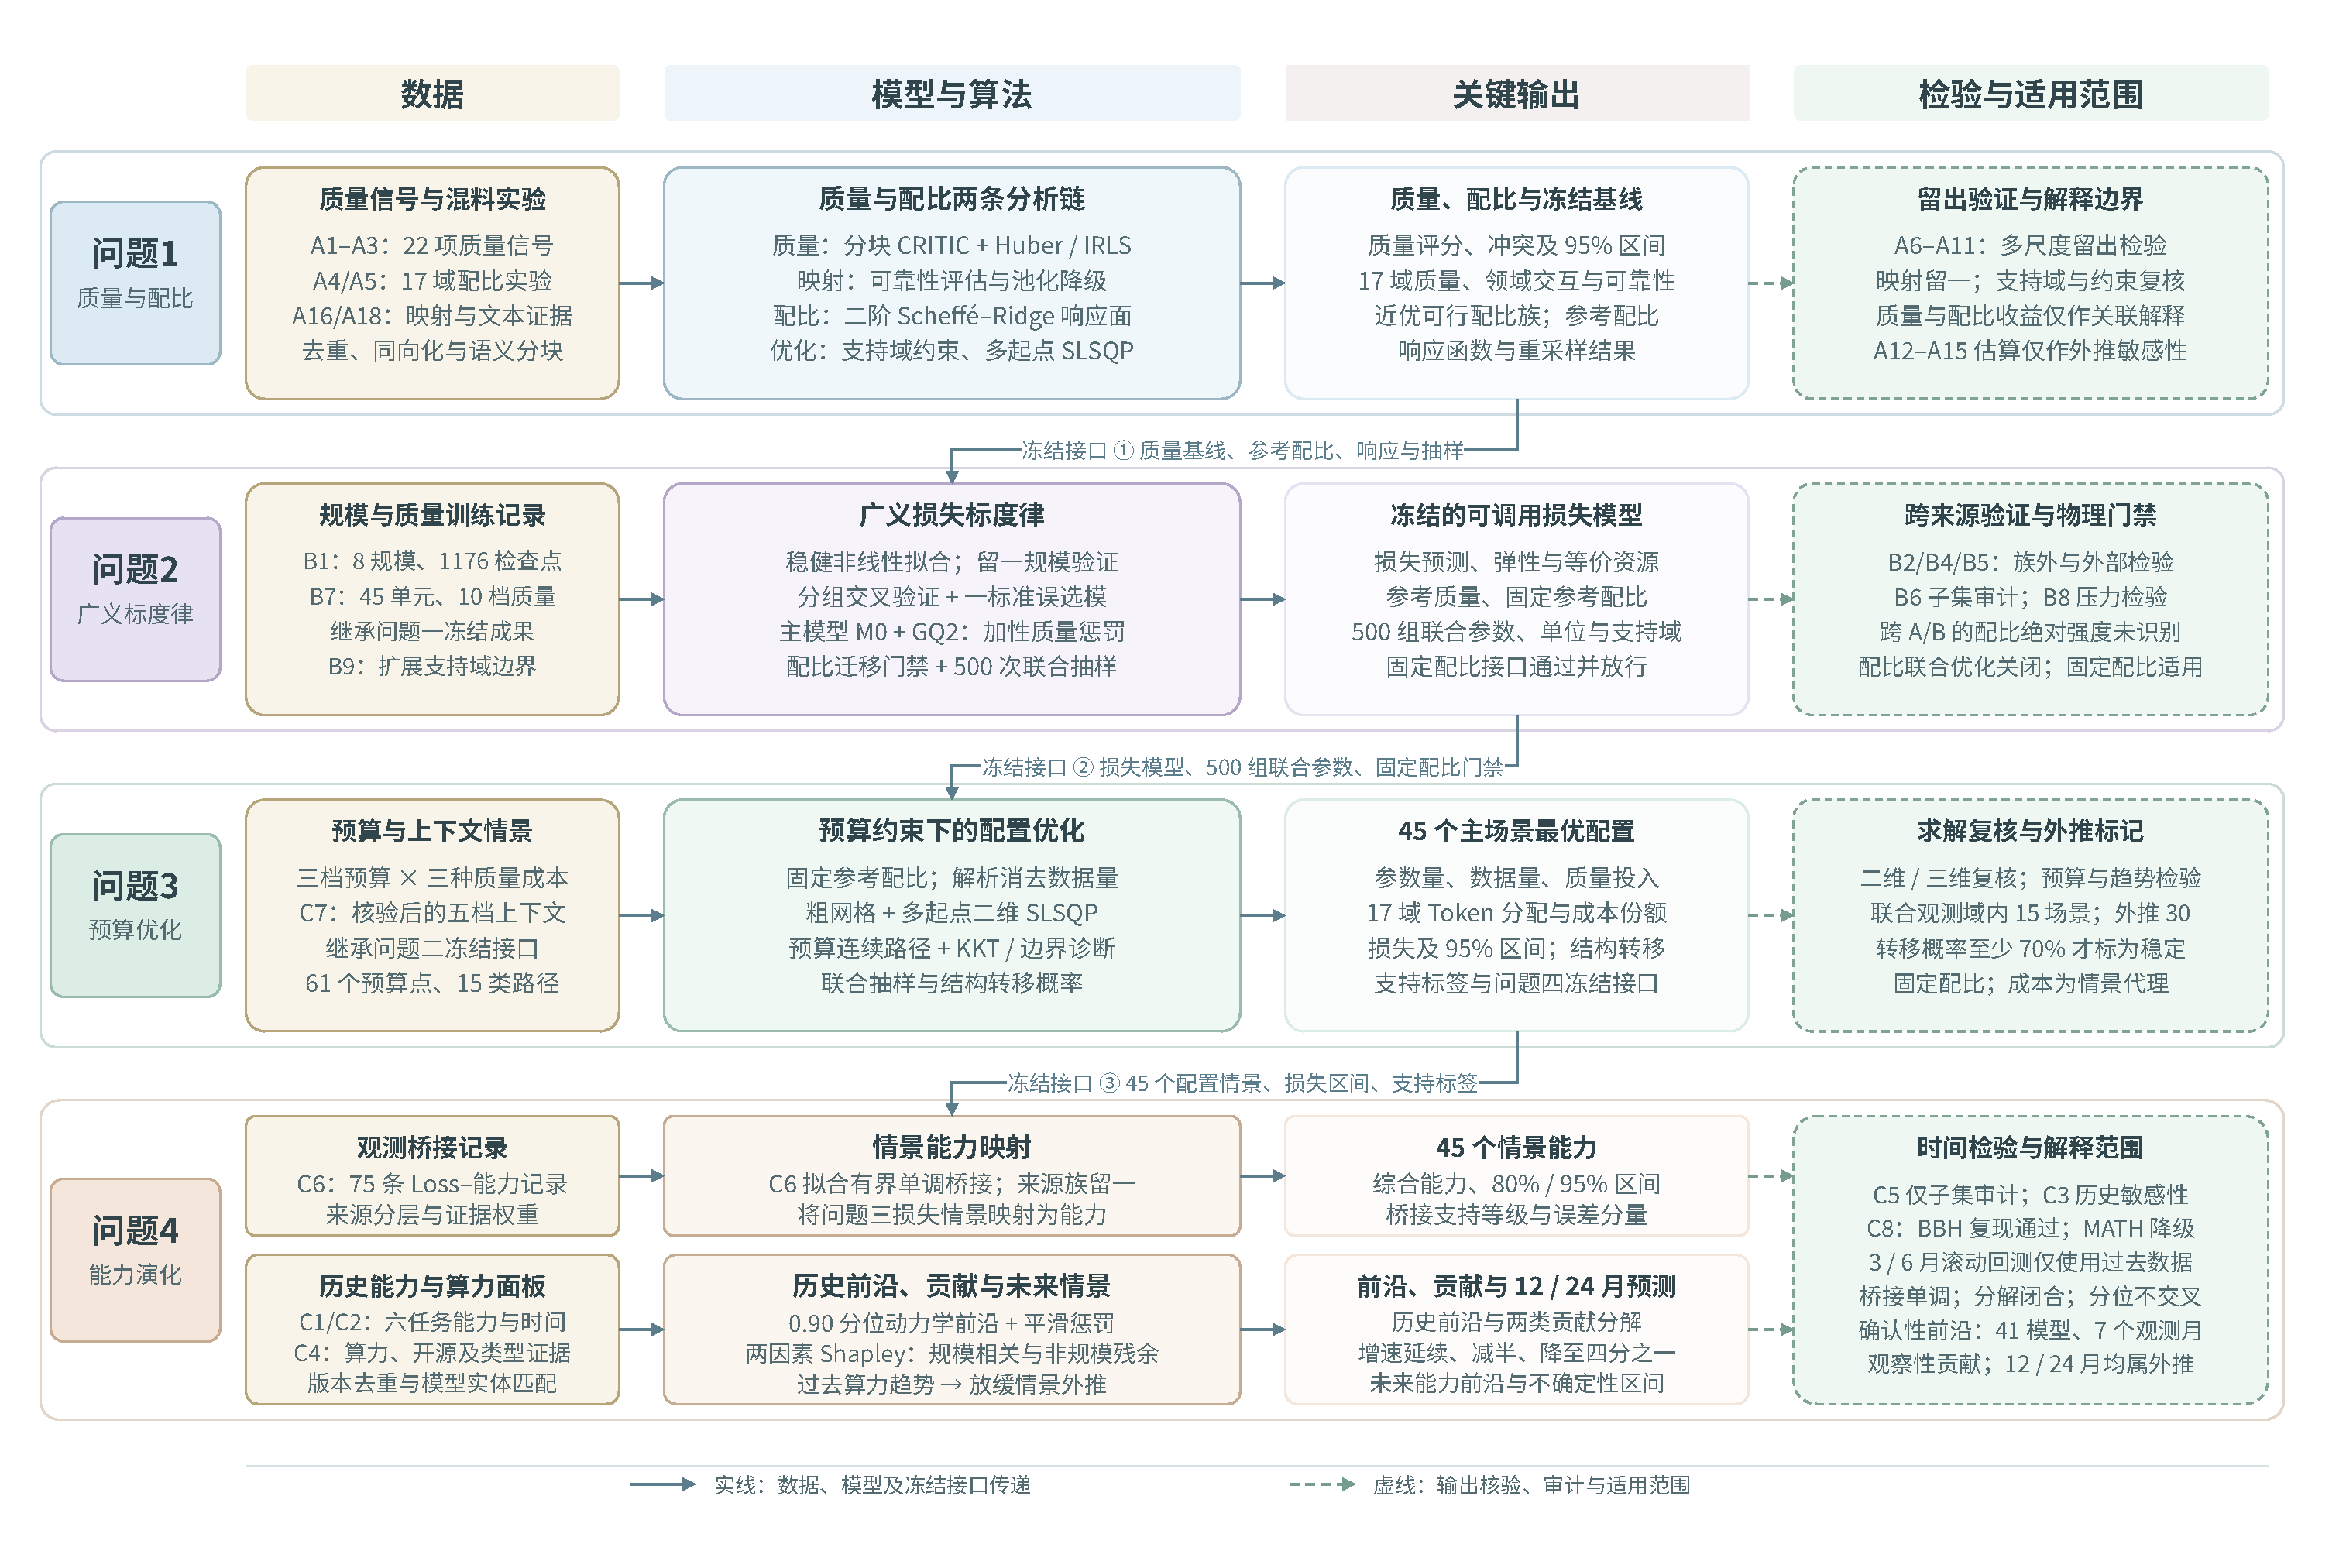
\includegraphics[width=0.98\linewidth]{images/F00_四问关系.pdf}
\caption{四个问题的数据依赖、模型接口与验证关系}
\label{fig:overall_dependency}
\end{figure}

图~\ref{fig:overall_dependency} 中，横向链条表示每一问从数据到模型、输出和检验的内部闭环，纵向连线表示跨问题传递的冻结接口。实线用于模型计算和已验收结果传递，虚线用于跨来源映射、敏感性分析或适用边界检查。特别地，问题一的近优配比 $\boldsymbol p^\star$ 只用于候选方案和方向判断；问题二、三的主链固定 $\boldsymbol p=\boldsymbol p_{\mathrm{ref}}$，从而避免把尚未识别的跨体系配比强度写入中心决策。

\subsection{问题三求解框架}

问题三承接前两问时，先检查冻结标度律、参考配比和上下文证据是否满足接口门槛，再在不同预算、质量成本和上下文情景下求解中心配置；随后沿连续预算路径识别结构转移，并以独立复核、联合抽样和支持域标签完成验收。该过程按“冻结接口--预算优化--路径诊断”分为三层，如图~\ref{fig:p3_overall_framework}所示。

\begin{figure}[H]
\centering
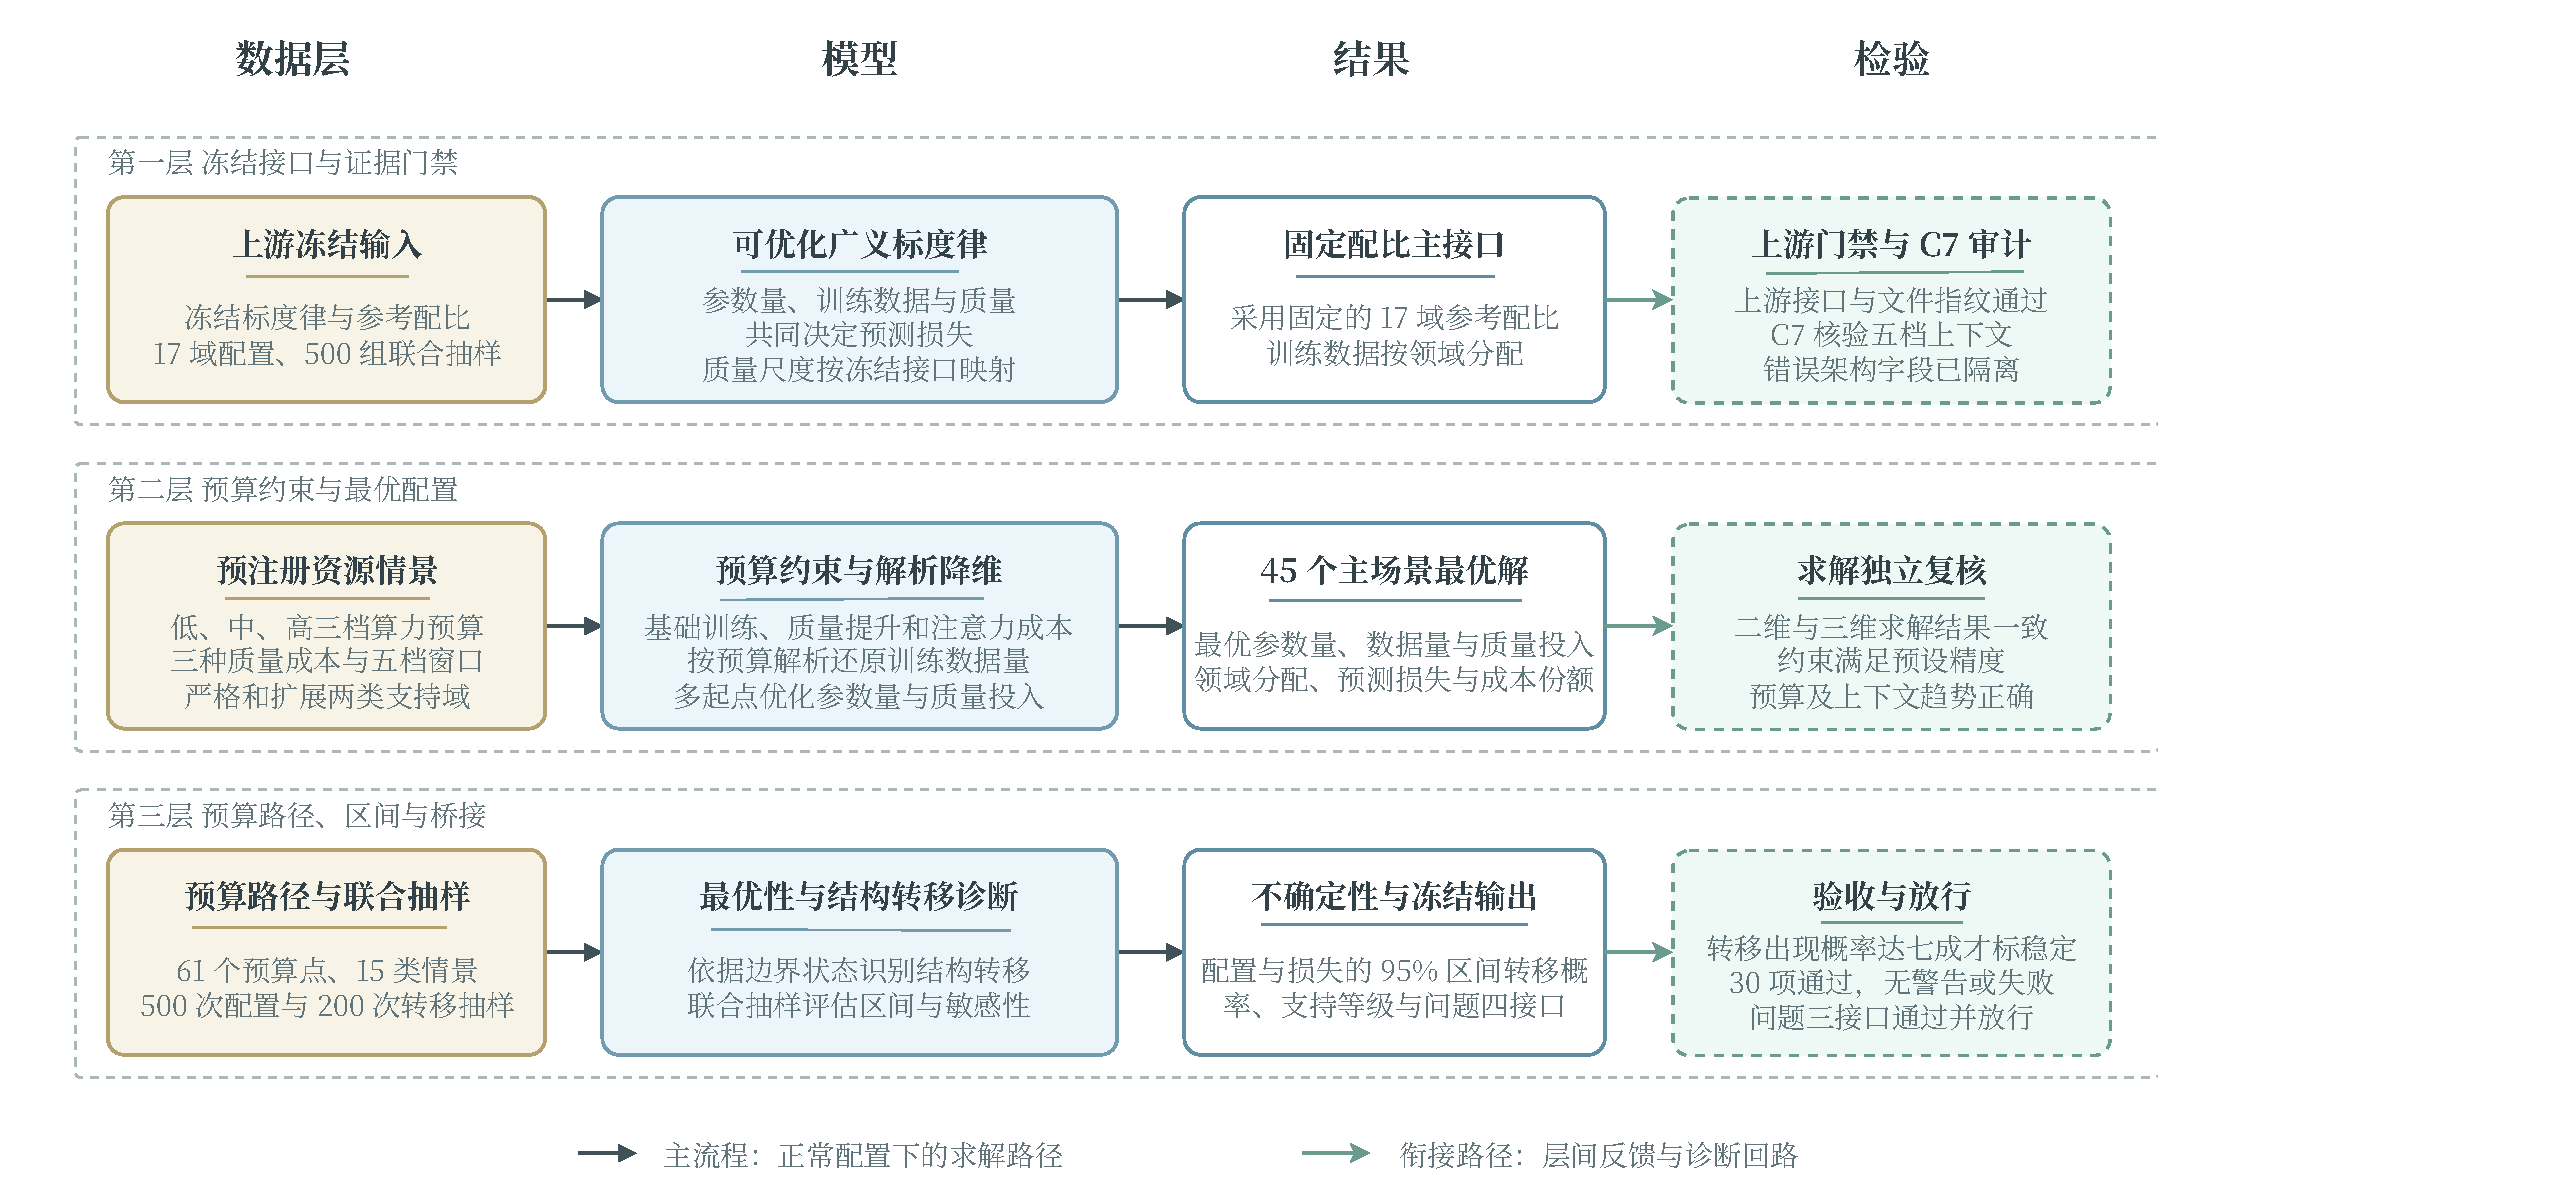
\includegraphics[width=0.98\linewidth]{images/no3/P3_F00R_问题三框架图.pdf}
\caption{问题三从冻结接口到优化验收的分层建模框架}
\label{fig:p3_overall_framework}
\end{figure}

该框架把中心求解与证据审计并列组织：中心链输出参数量、数据量、质量投入和领域 Token 分配，诊断链同时报告约束可行性、求解一致性、结构转移概率与外推等级。由此，问题三输出的不只是一个最优点，而是带有适用范围和不确定性说明的条件最优配置。


\section{问题一模型的建立与求解}
\label{sec:problem1}

\subsection{问题分析与建模思路}

问题一包含数据质量评价与训练数据配比优化两个相互关联的任务。前者利用附件 A1--A3 的多维质量信号回答“文本本身具有怎样的质量结构”，后者利用附件 A4--A15 的配比实验回答“领域组成如何改变模型验证损失”。两类附件的统计对象和监督信息不同：质量附件以文本为观测单位，配比附件以训练配方为观测单位，二者不能逐行拼接。因此，本文分别建立质量评价模型和配比响应模型，再借助 A16、A18 将质量域映射到配方域，作为解释性联系而非额外监督标签。

设第 $i$ 个配方域的比例与领域质量分别为 $p_i$ 和 $q_i$。由于 $\sum_i p_iq_i$ 是 $p_i$ 的线性组合，若将其与全部 Scheff\'e 一次项同时放入响应模型，就无法从现有配比实验中区分“领域组成效应”和“静态质量效应”。此外，A18 只提供文本及领域标签，并不包含 A1--A3 的完整质量信号。基于这两点，领域质量只用于解释配方特征和检验质量排序与训练收益是否一致；配比模型仍完全由配比--Loss 实验训练。

本问的技术路线为：先将 22 项异构质量信号转换到 $[0,1]$ 且统一为“越高越好”，再按质量含义构成五个语义块，通过稳定 CRITIC 权重与冲突自适应 Huber 估计得到样本质量 $Q_i$；随后在领域内稳健聚合并评估跨体系映射可靠性。配比侧则在单纯形上拟合二阶 Scheff\'e--Ridge 多输出响应面，通过 1M、60M 和 1B 实测配方检验模型的排序能力，最后在训练支持域内搜索近优可行配比，并用多起点和 bootstrap 量化求解不确定性。

上述两条建模链及其证据边界汇总于图~\ref{fig:p1_f00}。质量链输出样本分数、领域质量及映射可信度，配比链输出响应面、边际效应与近优可行配比；二者只在“质量--收益一致性检验”处作关联解释，避免把静态质量重复计入配比回归。图中的虚线表示验证、敏感性或关联分析，不参与主模型的数据传递。

\begin{figure}[htbp]
\centering
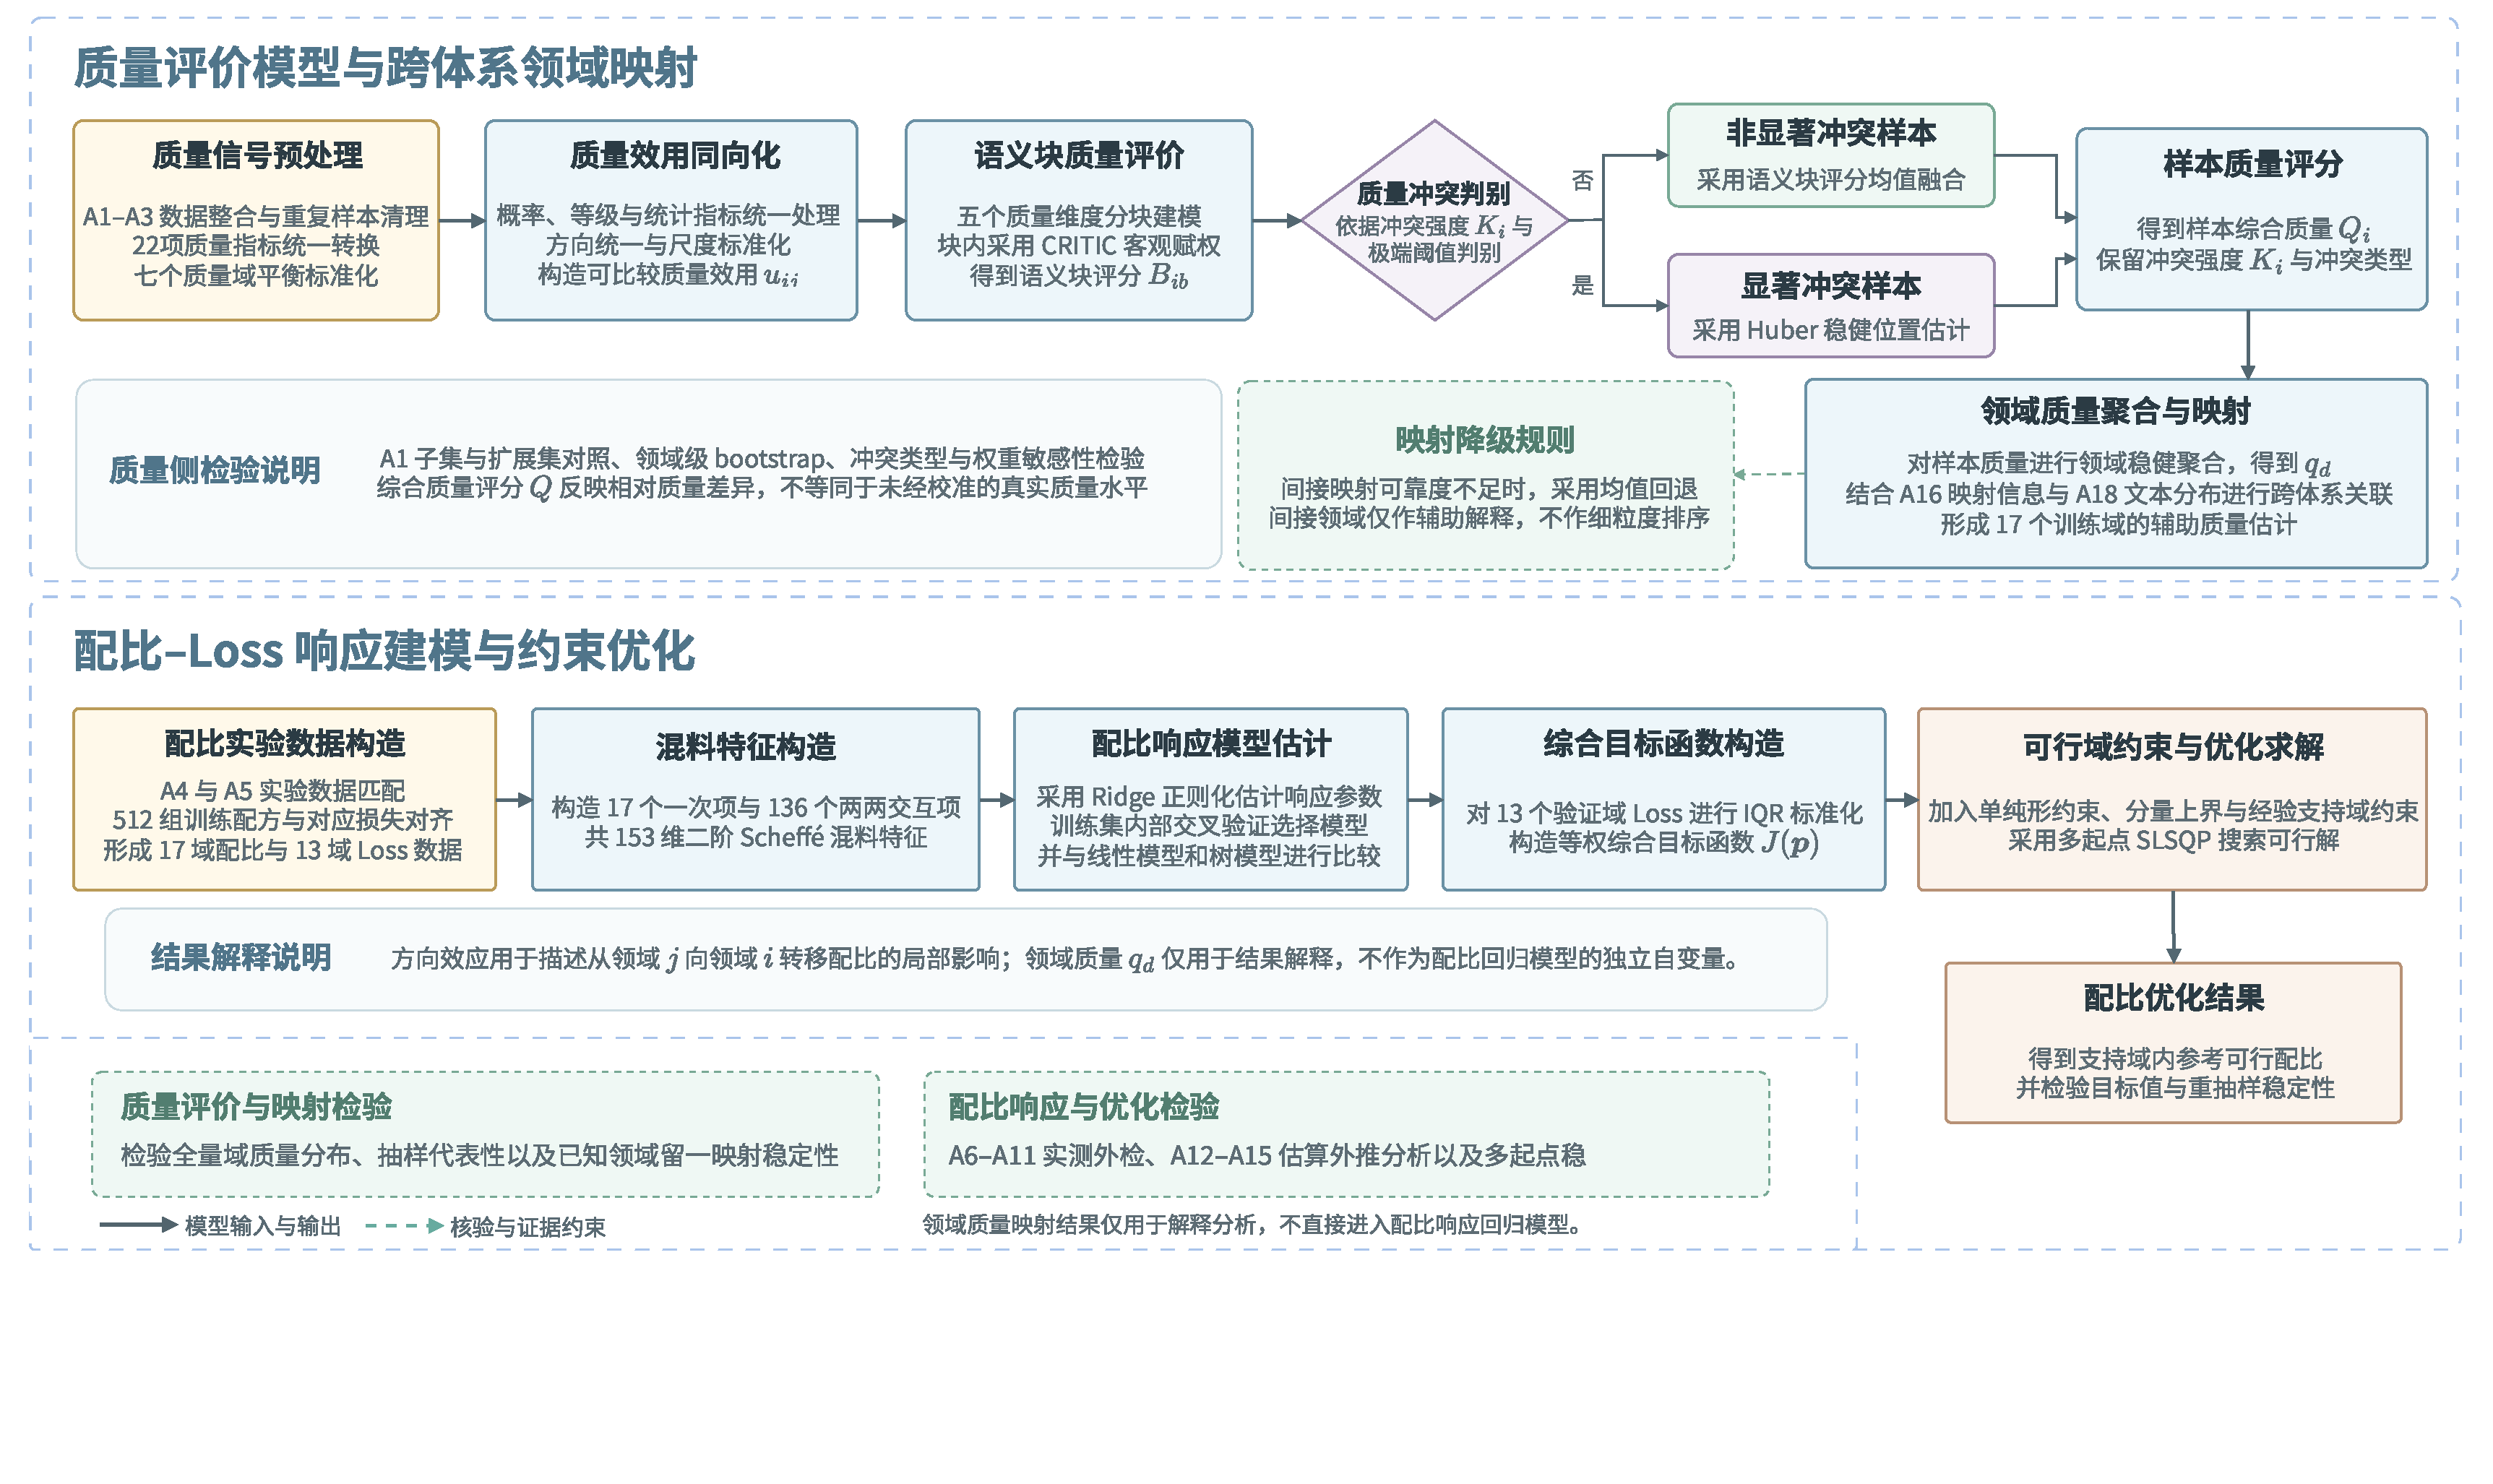
\includegraphics[width=0.97\linewidth]{images/no1/P1_F00R_问题一求解流程图.pdf}
\caption{问题一质量评价、领域映射与配比优化求解流程}
\label{fig:p1_f00}
\end{figure}

该框架最终形成四层可追溯结果：样本层保留 $Q_i$ 与冲突类型，领域层给出七域质量及 17 域映射区间，响应层保留 $\widehat L_k(\boldsymbol p)$ 与边际效应，决策层则给出带支持域和区间说明的近优配比族。后续各节依次给出这四层结果的构造与验证。

\subsection{输入、数据与证据边界}

\subsubsection{数据组织与预处理}

各附件的统计对象与分析角色见表~\ref{tab:p1_data_role}。质量侧以去重后的独立文本为统计单位；配比侧严格区分训练、实测检验和估算外推，测试数据不参与模型选择或正则化参数确定。

\begin{table}[htbp]
\centering
\small
\setlength{\tabcolsep}{5pt}
\caption{问题一主要数据及其分析角色}
\label{tab:p1_data_role}
\begin{tabular}{p{0.14\linewidth}p{0.29\linewidth}p{0.45\linewidth}}
\toprule
附件 & 统计对象 & 用途 \\
\midrule
A1--A3 & $51230$、$17523$、$203752$ 条质量记录 & 22 项质量信号转换、冲突分析、七域质量评价及扩展集检验 \\
A4/A5 & $512$ 组训练配方及 13 域 Loss & 配比响应面训练、内部交叉验证与模型选择 \\
A6/A7 & $256$ 组 1M 实测配方 & 同规模独立检验 \\
A8/A9 & $256$ 组 60M 实测配方 & 相同配方下的跨规模检验 \\
A10/A11 & $64$ 组 1B 实测配方 & 独立配方、独立规模检验 \\
A12--A15 & 10B、70B 各 $63$ 组估算配方 & 外推敏感性分析，不参与主模型训练与选模 \\
A16/A18 & 领域映射指引与 17 域文本样本 & 质量域到配方域的辅助映射及可靠性检验 \\
\bottomrule
\end{tabular}
\end{table}

A1 与 A2、A3 分别有 $1419$ 条 arXiv 记录和 $10000$ 条 GitHub 记录重合。本文以规范化领域名和样本标识联合去重，并核对重合记录的质量字段；未发现同标识质量冲突。最终质量参考集包含 $261086$ 条独立记录。原始数据中的少量非有限值保留为缺失，不做均值插补；样本评分仅使用其有效指标，并在块内重新归一权重，避免人为补值改变评价方向。

配比表与 Loss 表按 \texttt{index} 一一匹配。设第 $r$ 组实验中第 $i$ 个领域的原始份额为 $a_{ri}$，对存储精度引起的微小闭合误差作非负修正和重新归一化：
\begin{equation}
p_{ri}=\frac{\max(a_{ri},0)}{\sum_{j=1}^{17}\max(a_{rj},0)},
\qquad p_{ri}\ge 0,
\qquad \sum_{i=1}^{17}p_{ri}=1.
\label{eq:p1_closure}
\end{equation}
闭合后的最大行和误差为 $4.44\times10^{-16}$。训练配方包含 17 个领域比例和 13 个验证域 Loss；全部 17 个比例均作为组成变量保留，即使某些训练领域没有同名验证列，其作用仍可通过多输出响应面识别。

\subsection{模型建立}

\subsubsection{指标同向化与五语义块构建}

质量信号同时包含连续统计量、模型概率、有序分类输出和列表型评分。本文先将二分类 logits 转为正类概率，将六级分类 logits 转为有序期望，并将 QuRating 四个分量分别转换后取均值，最终得到题目要求的 22 项质量指标。所有效用均记为 $u_{ij}\in[0,1]$，且数值越大表示当前指标意义下的质量越高。

为避免 GitHub 等大样本领域主导经验标尺，对需作秩变换的指标 $j$，先在七个质量域内分别估计经验分布，再等权构造平衡参考分布
\begin{equation}
F_j^{\mathrm{bal}}(x)=\frac{1}{7}\sum_{d=1}^{7}F_{jd}(x).
\label{eq:p1_balanced_cdf}
\end{equation}
变换前按该平衡分布的 $0.5\%$ 和 $99.5\%$ 分位截尾。正向指标取 $u_{ij}=F_j^{\mathrm{bal}}(x_{ij})$，逆向指标取 $u_{ij}=1-F_j^{\mathrm{bal}}(x_{ij})$。词元熵与独特词比例具有边际收益递减特征，故采用饱和效用
\begin{equation}
u_{ij}=\min\left\{\frac{F_j^{\mathrm{bal}}(x_{ij})}{0.95},1\right\}.
\label{eq:p1_saturating_utility}
\end{equation}

文本长度、句子数和平均词长并非越大越好。对这类结构指标先作 $z_{ij}=\log(1+\max\{x_{ij},0\})$，再在高流畅、低广告且高整洁的可信样本中，以七域平衡方式估计中心 $m_j$ 和稳健尺度 $s_j$，定义中间型效用
\begin{equation}
u_{ij}=\exp\left[-\frac{(z_{ij}-m_j)^2}{2s_j^2}\right].
\label{eq:p1_mid_utility}
\end{equation}
数字字符比例具有明显领域依赖性：GitHub 中的数字和符号常属于正常代码结构，故使用中间型效用；其余自然语言领域仍按逆向指标处理。已经位于 $[0,1]$ 且方向明确的模型概率和有序期望不再重复作秩变换，以保留概率间距。

根据指标含义，22 项信号被划分为教育与领域价值、表达与整洁、推理与信息、噪声与重复、结构充分性五个语义块。先在块内融合，再在块间等权，可避免某一语义块仅因包含指标较多而获得更大总权重。

\subsubsection{稳定 CRITIC 赋权与质量冲突消解}

在同向化之后，指标间仍存在显著的信息重叠。本文在每个语义块内采用 CRITIC 思想确定客观权重\cite{diakoulaki1995critic}。为平衡领域样本量，每域最多等概率抽取 $10000$ 条记录。设指标 $j$ 的标准差为 $\sigma_j$，与同块指标 $h$ 的 Spearman 相关为 $r_{jh}$，则其信息量为
\begin{equation}
C_j=\sigma_j\sum_{h\in\mathcal J_b}(1-|r_{jh}|).
\label{eq:p1_critic_information}
\end{equation}
绝对相关同时惩罚强正相关和强负相关造成的信息重复。进一步在 500 次分层 bootstrap 中计算指标跨领域位置统计量的变异系数 $\mathrm{CV}_j$，得到稳定性修正后的块内权重
\begin{equation}
\omega_j=
\frac{C_j/(1+\mathrm{CV}_j)}
{\sum_{h\in\mathcal J_b}C_h/(1+\mathrm{CV}_h)},
\qquad \sum_{j\in\mathcal J_b}\omega_j=1.
\label{eq:p1_critic_weight}
\end{equation}

图~\ref{fig:p1_f01}给出 22 项同向化指标的相关结构及最终综合权重。图中若干指标形成明显相关簇，例如图书、百科和数学相似度之间高度相关；稳定 CRITIC 权重因此不会把同一类信息重复计入。平均词长的综合权重约为 $0.0899$，但五类语义块仍各占总评分的 $1/5$，不存在由单一指标直接决定综合质量的情形。

\begin{figure}[htbp]
\centering
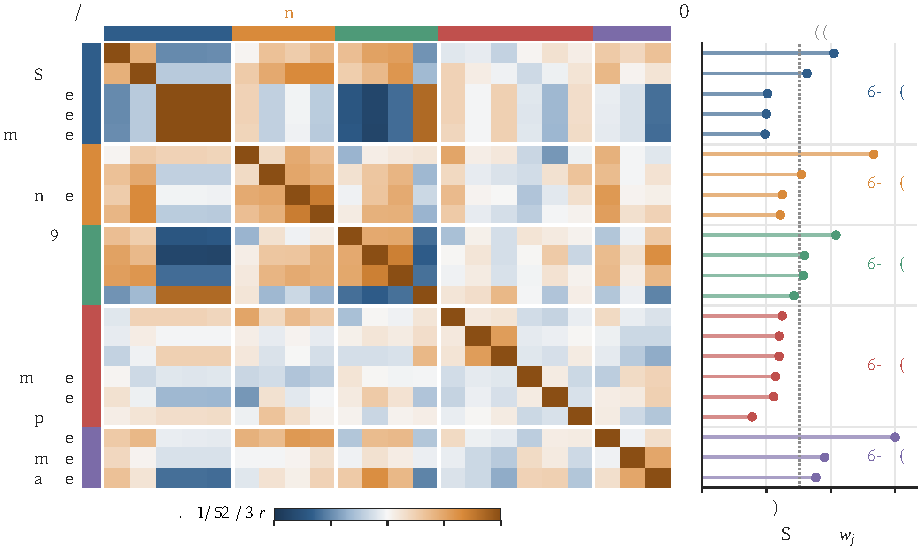
\includegraphics[width=0.98\linewidth]{images/no1/P1_F01_质量指标结构与权重.pdf}
\caption{质量指标相关结构与稳定 CRITIC 权重}
\label{fig:p1_f01}
\end{figure}

记 $\mathcal O_i$ 为样本 $i$ 的有效指标集合，$\mathcal J_b$ 为语义块 $b$ 的指标集合，则块评分为
\begin{equation}
B_{ib}=\frac{\sum_{j\in\mathcal J_b\cap\mathcal O_i}\omega_j u_{ij}}
{\sum_{j\in\mathcal J_b\cap\mathcal O_i}\omega_j}.
\label{eq:p1_block_score}
\end{equation}
若某块没有有效指标则记为缺失，不生成替代值。最终数据中没有样本出现整块缺失。

为识别“某一维度很高、另一维度很低”的内部矛盾，定义块间极差 $K_i=\max_b B_{ib}-\min_b B_{ib}$。当 $K_i$ 高于所属领域的 $90\%$ 分位，且同时满足 $\max_b B_{ib}\ge0.75$、$\min_b B_{ib}\le0.25$ 时，将样本标记为显著冲突。非冲突样本取有效块均值；冲突样本采用 Huber 稳健位置估计\cite{huber1964robust}：
\begin{equation}
Q_i=
\begin{cases}
|\mathcal B_i|^{-1}\displaystyle\sum_{b\in\mathcal B_i}B_{ib}, & i\notin\mathcal C,\\[6pt]
\displaystyle\arg\min_{q\in[0,1]}
\sum_{b\in\mathcal B_i}\frac{1}{|\mathcal B_i|}
\rho_{1.345}\!\left(\frac{B_{ib}-q}{s_{db}}\right), & i\in\mathcal C,
\end{cases}
\label{eq:p1_quality_score}
\end{equation}
其中 $\mathcal B_i$ 为有效块集合，$\mathcal C$ 为显著冲突样本集合，$s_{db}$ 为领域 $d$ 中块 $b$ 的 MAD 稳健尺度，$\rho_c$ 为 Huber 损失。该机制不删除冲突信息，而是同时保存 $K_i$、冲突方向和冲突标记，用于解释评分差异。

在 $261086$ 条记录中，显著冲突率为 $3.17\%$。图~\ref{fig:p1_f04}显示，较常见的冲突包括“推理信息高、结构充分低”“噪声重复高、结构充分低”和“表达整洁高、结构充分低”。Huber 修正对 $252816$ 个非冲突样本近似为零；对 $8270$ 个冲突样本，修正量均值约为 $0.0773$、中位数约为 $0.0376$，说明稳健估计主要调整内部不一致样本，而非改变全部样本的评分基线。

\begin{figure}[htbp]
\centering
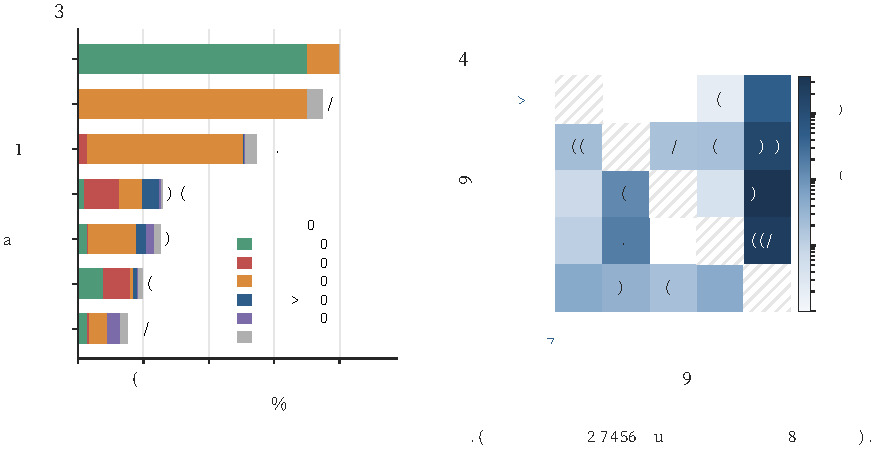
\includegraphics[width=0.96\linewidth]{images/no1/P1_F04_质量冲突机制与稳健消解.pdf}
\caption{质量冲突结构与 Huber 稳健修正效应}
\label{fig:p1_f04}
\end{figure}

\subsubsection{领域质量评价与跨体系映射}

样本质量范围为 $0.140735$--$0.880183$。对领域 $d$ 的样本集合 $\mathcal S_d$，本文使用领域内质量分数的 Huber 稳健均值，而不是简单均值或中位数：
\begin{equation}
q_d=\arg\min_q\sum_{i\in\mathcal S_d}
\rho_{1.345}\!\left(\frac{Q_i-q}{s_d}\right),
\label{eq:p1_domain_quality}
\end{equation}
其中 $s_d$ 为领域内 $Q_i$ 的 MAD 尺度。每个领域独立进行 500 次 bootstrap，取 $2.5\%$ 和 $97.5\%$ 分位作为不确定区间。表~\ref{tab:p1_quality}显示，C4 和 Common Crawl 在当前指标体系中的中心质量较高，GitHub 相对较低；这些结果反映质量信号空间中的相对位置，不等同于人工标注意义下的绝对文本价值。

\begin{table}[htbp]
\centering
\small
\setlength{\tabcolsep}{4pt}
\caption{七个质量域的稳健质量及显著冲突率}
\label{tab:p1_quality}
\begin{tabular}{lrrrr}
\toprule
领域 & 样本数 & 领域质量 $q_d$ & bootstrap 95\% 区间 & 冲突率/\% \\
\midrule
C4 & 10000 & 0.6192 & [0.6173, 0.6210] & 6.83 \\
Common Crawl & 9640 & 0.6083 & [0.6067, 0.6097] & 1.88 \\
arXiv & 17523 & 0.5688 & [0.5679, 0.5697] & 10.00 \\
Stack Exchange & 10000 & 0.5608 & [0.5591, 0.5624] & 3.14 \\
Book & 171 & 0.5100 & [0.4995, 0.5215] & 9.36 \\
Wikipedia & 10000 & 0.5067 & [0.5047, 0.5084] & 3.22 \\
GitHub & 203752 & 0.4304 & [0.4301, 0.4306] & 2.45 \\
\bottomrule
\end{tabular}
\end{table}

在使用扩展集给出最终域质量之前，需要检查 A1 抽样记录能否代表 A2/A3 的去重余集。图~\ref{fig:p1_f03}比较了 arXiv 和 GitHub 两域的经验分布差与分位数位移。两域的 KS 距离分别为 $0.025$ 和 $0.011$，Wasserstein 距离分别为 $0.0029$ 和 $0.0011$；Huber 均值差的 bootstrap 区间均跨越零。主体分布未见稳定偏移，但 arXiv 约第 $90$ 百分位处仍存在约 $0.076$ 的局部位移且区间较宽。因此，A1 对两域主体分布具有一定代表性，但不能据此宣称高质量尾部完全等价。

\begin{figure}[htbp]
\centering
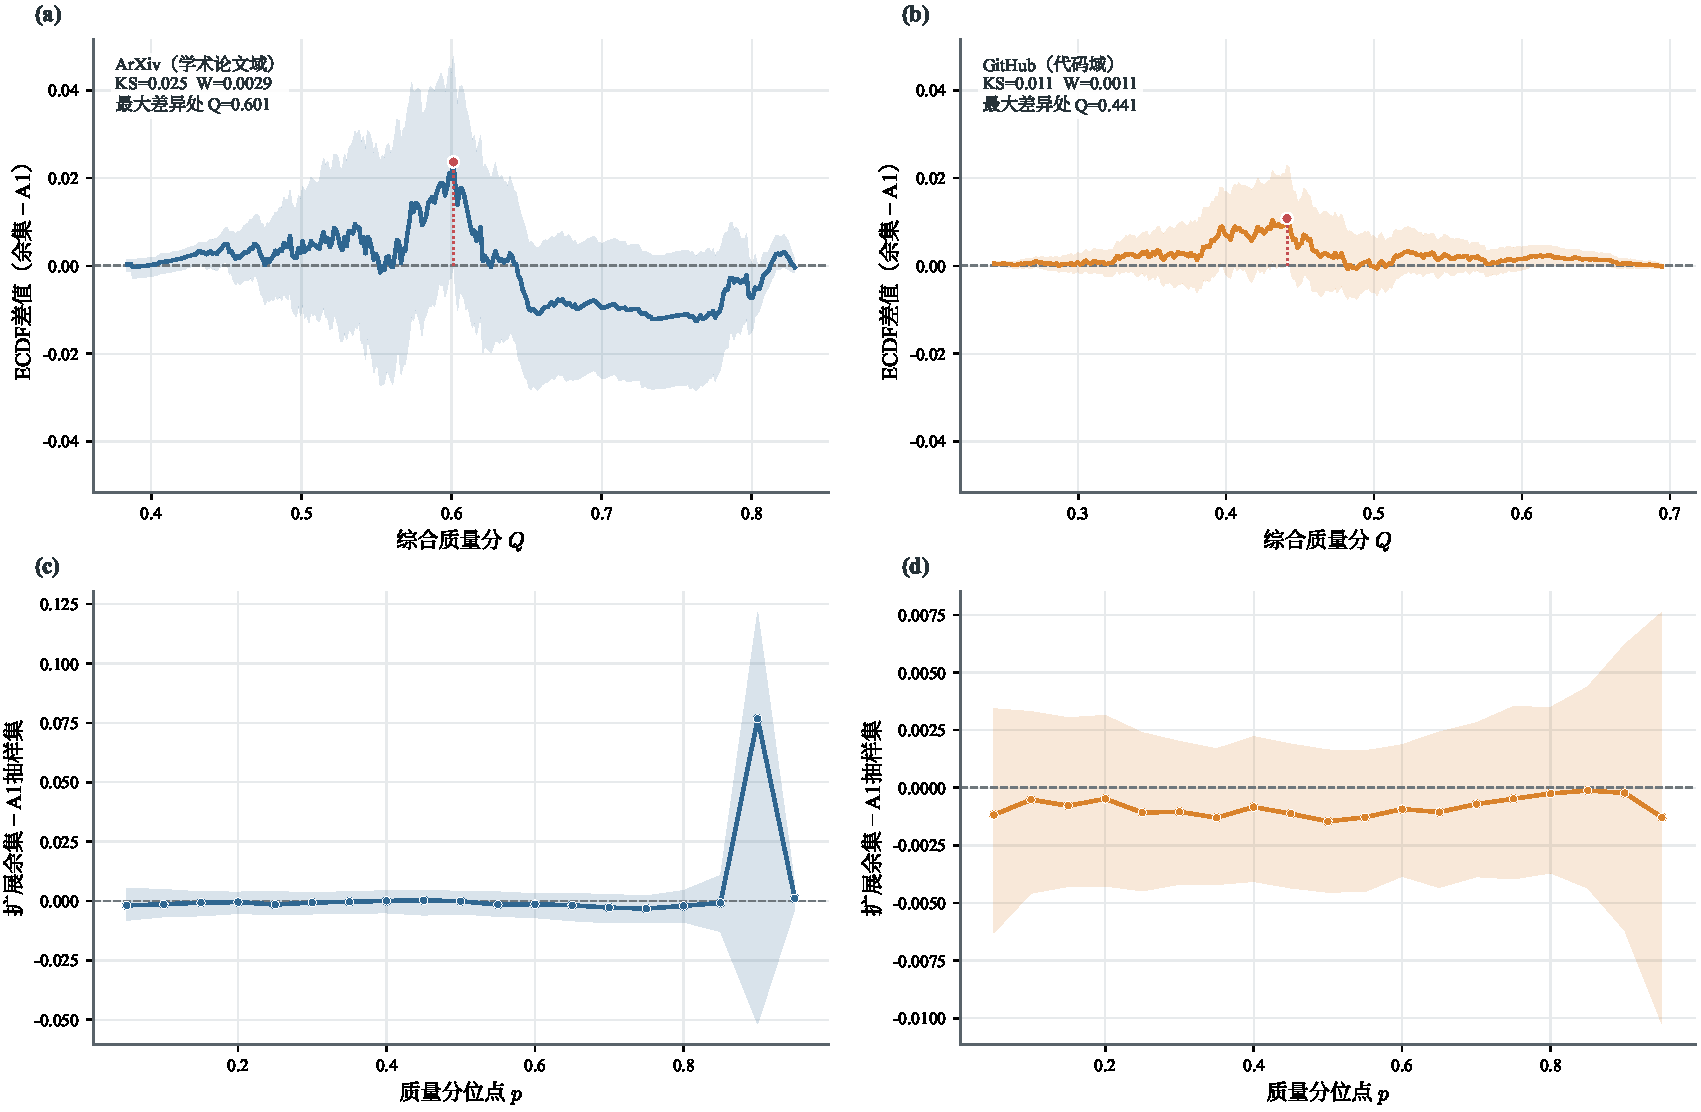
\includegraphics[width=0.98\linewidth]{images/no1/P1_F03_扩展集代表性诊断.pdf}
\caption{A1 抽样集相对扩展余集的分布代表性诊断}
\label{fig:p1_f03}
\end{figure}

质量附件覆盖七个领域，而配比模型使用 17 个 The Pile 领域。对 direct 和 near\_direct 映射，直接采用对应质量锚点；其余领域由 A18 文本的长度、字符、结构和重复特征与七个锚点进行距离匹配。设 $d_{md}$ 为配方域 $m$ 到质量域 $d$ 的标准化文本分布距离，温度参数为 $\tau$，则软映射权重与收缩估计为
\begin{equation}
w_{md}=\frac{\exp[-(d_{md}-d_{m,\min})/\tau]}
{\sum_{h=1}^{7}\exp[-(d_{mh}-d_{m,\min})/\tau]},
\quad
q_m=\lambda_m\sum_{d=1}^{7}w_{md}q_d+(1-\lambda_m)\bar q.
\label{eq:p1_mapping}
\end{equation}
其中 $\bar q$ 为七域质量均值。$\tau$ 只通过已知域留一误差选择；若留一排序达到预设可靠门槛，$\lambda_m$ 随 A18 样本量增加而增大、随最近锚点距离增加而减小，否则置为零。

最终选择 $\tau=5$，已知域留一 MAE 为 $0.056933$，但 Spearman 系数为 $-1$，不足以支持对推断域作稳定排序。因此，11 个推断域的 $\lambda_m$ 均置为零，并回退到公共参考质量 $\bar q=0.543464$。该值的 bootstrap 主区间约为 $[0.541887,0.545099]$；映射假设变化得到的 $[0.409869,0.677059]$ 仅作为敏感性包络，不能解释为真实质量的 95\% 置信区间。

图~\ref{fig:p1_f02}同时展示七域质量分布和 17 域映射证据。左侧山脊下方的点带为每域最多 500 个样本的固定随机抽样，用于辨认局部聚集、偏态和尾部结构；山脊上的三条标记依次对应 P5、中位数和 P95，因此点带仅辅助阅读，不参与领域质量估计。右侧连线宽度表示映射权重，颜色区分映射证据等级。17 个配方域中有 3 个直接映射、3 个近直接映射和 11 个推断映射。直接与近直接领域保留锚点差异；推断领域的共同数值只表示当前证据不足以区分，而非其真实质量相同。

\begin{figure}[htbp]
\centering
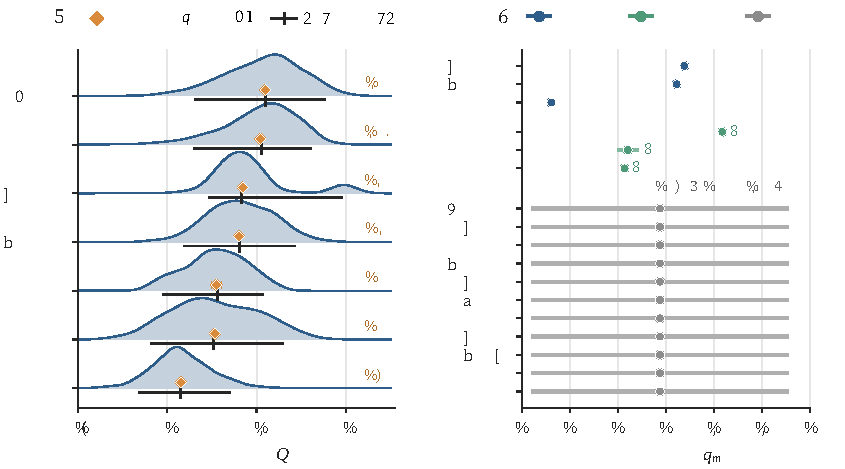
\includegraphics[width=0.98\linewidth]{images/no1/P1_F02_领域质量景观与映射.pdf}
\caption{七域质量分布、样本点带及其向 17 个配方域的映射}
\label{fig:p1_f02}
\end{figure}

为检验质量评分对聚合规则的敏感性，本文在不重新调参的条件下比较指标等权、块内等权、取消 Huber 和块中位数等方案。七域排序相对于主模型的最小 Kendall 系数为 $0.8095$，但样本高、低质量极端组的最低重合率仅为 $0.613$。因此，领域层面的总体差异具有一定稳定性，单个文本的精细排名则对融合规则更敏感，本文不将样本级排名解释为绝对质量顺序。

\subsubsection{Scheff\'e--Ridge 配比响应模型}

17 个领域份额满足式~\eqref{eq:p1_closure}，属于单纯形上的组成数据。普通含截距回归会因 $\sum_i p_i=1$ 产生线性依赖，故本文采用无截距二阶 Scheff\'e 混料模型\cite{scheffe1958mixtures}。对第 $k$ 个验证域，预测损失为
\begin{equation}
\widehat L_k(\boldsymbol p)
=\sum_{i=1}^{17}\beta_{ik}p_i
+\sum_{1\le i<j\le17}\beta_{ijk}p_ip_j,
\qquad k=1,\ldots,13.
\label{eq:p1_scheffe}
\end{equation}
模型包含 17 个一次项和 $\binom{17}{2}=136$ 个交互项，共 153 个特征。一次系数描述给定混料曲面中的基础响应，交互系数描述两个领域共同变化时的非加性关系；二者均是统计关联，不代表因果贡献。

记 $\boldsymbol X_s$ 为按训练折均方根尺度标准化后的 Scheff\'e 设计矩阵，$\boldsymbol Y\in\mathbb R^{n\times13}$ 为 13 个验证域 Loss。采用多输出 Ridge 稳定高维系数估计\cite{hoerl1970ridge}：
\begin{equation}
\widehat{\boldsymbol B}
=\arg\min_{\boldsymbol B}
\left\|\boldsymbol Y-\boldsymbol X_s\boldsymbol B\right\|_F^2
+\lambda\left\|\boldsymbol B\right\|_F^2.
\label{eq:p1_ridge}
\end{equation}
\subsection{模型求解}

\subsubsection{响应面选择与局部效应求解}

在 A4/A5 内按配比结构进行五折分层交叉验证，标准化仅在各训练折估计。正则化强度以 13 域 IQR 标准化均方根误差最小为准。二阶 Ridge 的内部 NRMSE 为 $0.3959$，略优于 Elastic Net 的 $0.3986$、线性 Ridge 的 $0.4108$、Extra Trees 的 $0.4307$ 和随机森林的 $0.4423$，故将二阶 Ridge 冻结为主响应面。树模型的秩相关较高，仍作为非线性对照，不据此宣称 Ridge 在所有指标上占优。

图~\ref{fig:p1_f09}(a)进一步并列给出误差与排序指标。图中 Pareto 列只按“NRMSE 越小、Spearman 越大”两个目标判定，Kendall 仅作为补充指标，因而二阶 Ridge 与 Extra Trees 同时位于前沿并不矛盾：Extra Trees 的 Spearman 为 $0.8545$，但 NRMSE 为 $0.4307$；二阶 Ridge 的 Spearman 为 $0.8285$，却将 NRMSE 降至 $0.3959$，同时保留连续可微、可解释且便于约束寻优的响应面。图~\ref{fig:p1_f09}(b)显示二阶 Ridge 在 $\alpha^*=0.0562$ 处取得最小误差，且其附近存在 NRMSE 距最优值不超过 $1\%$ 的稳定区间，说明选定正则强度并非由单个尖锐网格点偶然决定。

\begin{figure}[htbp]
\centering
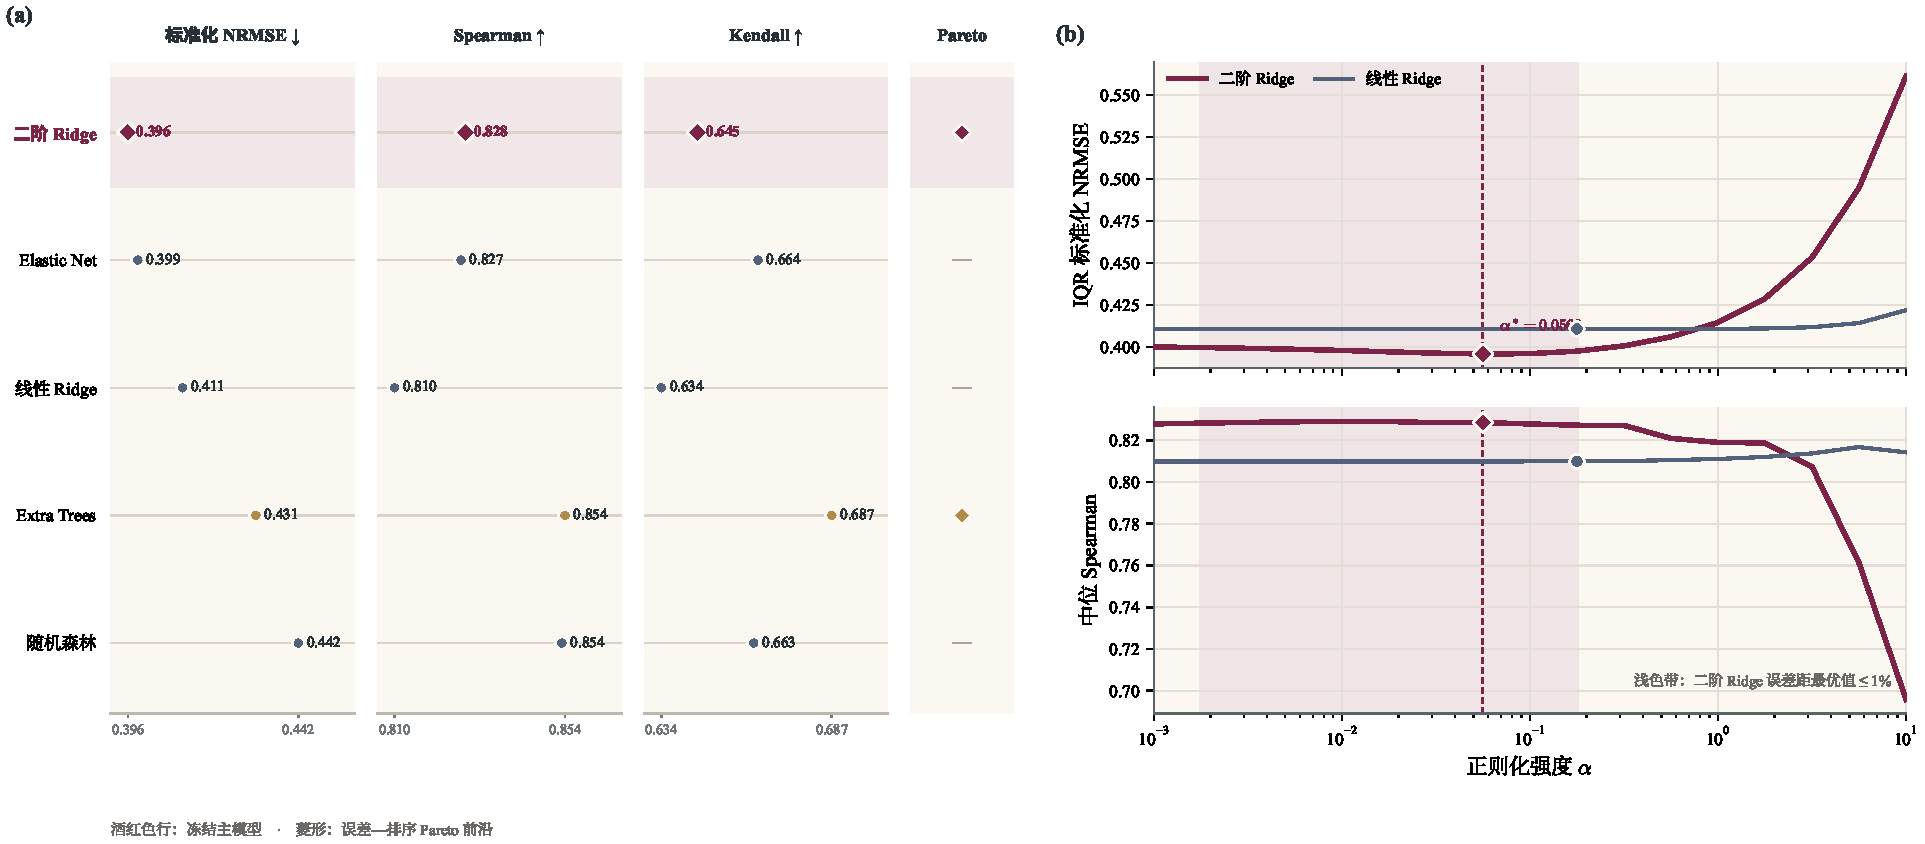
\includegraphics[width=0.98\linewidth]{images/no1/P1_F09_响应面选择与正则化诊断.pdf}
\caption{配比响应面的交叉验证选型与 Ridge 正则化诊断}
\label{fig:p1_f09}
\end{figure}

在组成约束下，单独增加某一份额必然压缩其他份额。为给出可解释的局部效应，在训练平均配比 $\boldsymbol p_{\mathrm{ref}}$ 处，将第 $i$ 个梯度相对于 17 域平均梯度中心化，并对 13 个验证域取均值。定义 Loss 下降方向的边际收益为
\begin{equation}
E_i=-\frac{1}{13}\sum_{k=1}^{13}
\left[
\frac{\partial\widehat L_k}{\partial p_i}
-\frac{1}{17}\sum_{j=1}^{17}
\frac{\partial\widehat L_k}{\partial p_j}
\right]_{\boldsymbol p=\boldsymbol p_{\mathrm{ref}}}.
\label{eq:p1_directional_effect}
\end{equation}
$E_i>0$ 表示在局部保持总比例不变时，向该领域转移份额与 Loss 下降相关。交互系数通过 500 次训练行 bootstrap 给出区间和符号稳定概率。

由于式~\eqref{eq:p1_directional_effect}只描述平均训练配比附近的一阶方向，本文进一步在 512 个训练配方上实施局部替换：按比例缩减其余 16 域，并向目标领域转入 $2\%$ 份额，再计算 13 个验证域的平均 Loss 降低量。图~\ref{fig:p1_f08}表明，同一领域的收益随参照配方显著变化。技术对话和数学推理的中位降低量分别为 $0.1072$ 和 $0.0657$，有利占比分别为 $91.2\%$ 和 $91.0\%$；商务邮件虽具有 $0.0973$ 的中位收益，但分布更宽，有利占比降至 $72.7\%$。哲学论文的中位效应仅为 $0.0044$，有利占比为 $52.3\%$，其 bootstrap 区间跨越零，不能据此给出稳定增配建议。

\begin{figure}[htbp]
\centering
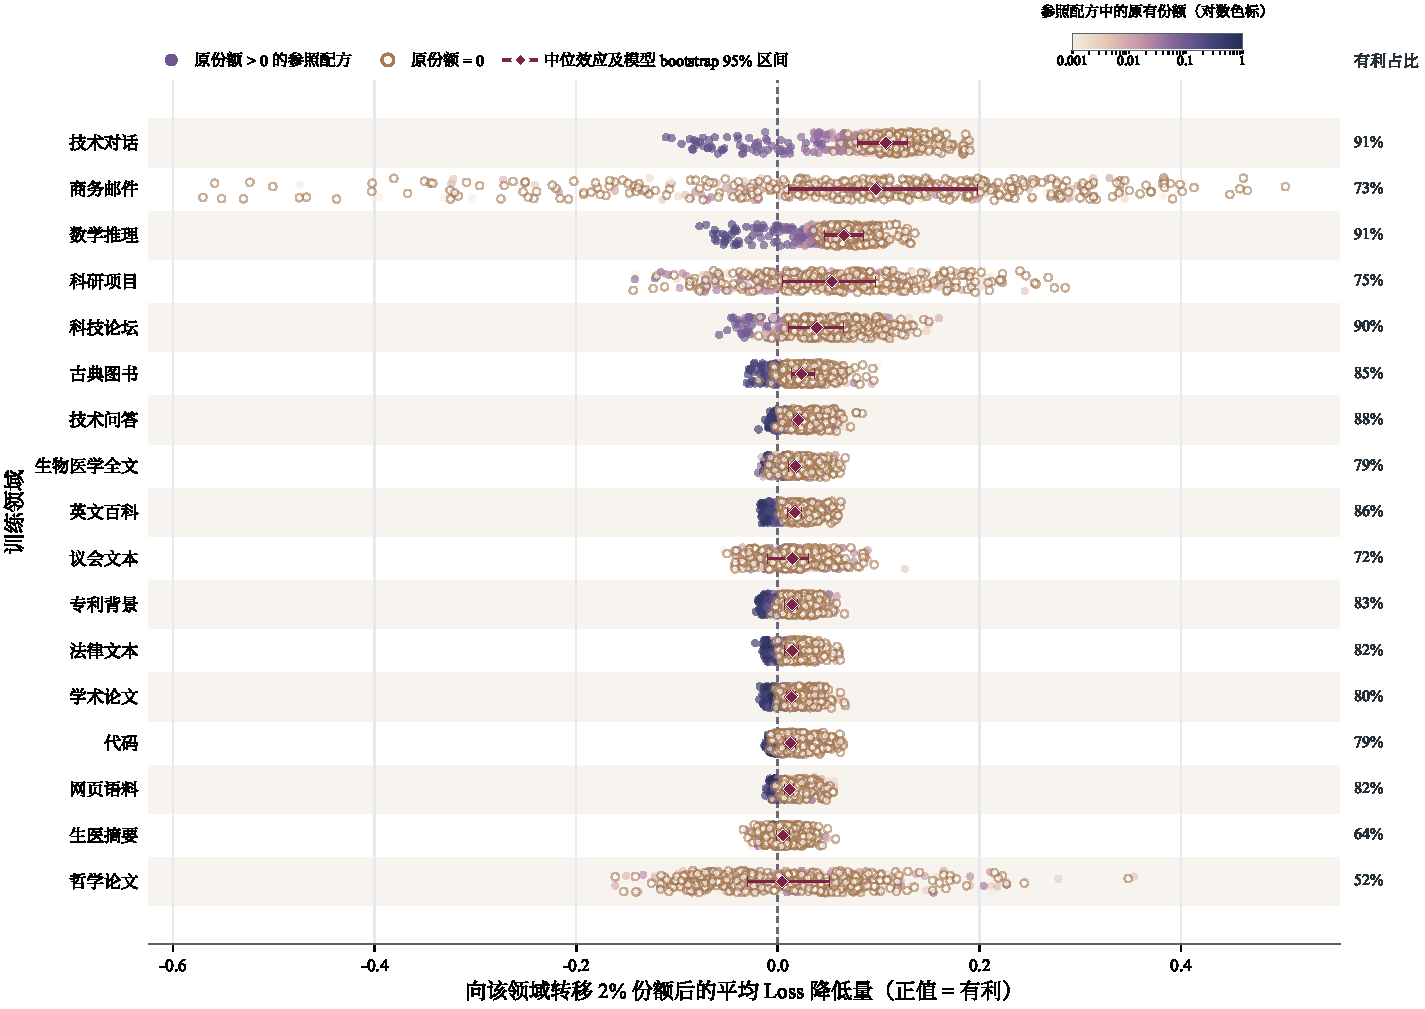
\includegraphics[width=0.94\linewidth]{images/no1/P1_F08_领域局部替换效应.pdf}
\caption{512 个训练配方上的领域局部替换效应}
\label{fig:p1_f08}
\end{figure}

图中多数领域的“原有份额--局部收益”相关为负，例如技术对话的 Spearman 系数为 $-0.662$，提示增配收益具有明显的起点依赖和边际递减特征。因此，领域效应应解释为给定组成附近的条件效应，而不能转化为脱离当前配方的固定领域排名。

\subsection{结果分析与模型验证}

\subsubsection{独立检验与跨尺度推广}

模型选择结束后，冻结的二阶 Ridge 一次性作用于 A6--A15。表~\ref{tab:p1_prediction}中的指标均为 13 个验证域的中位数；其中 1M、60M 和 1B 为实测检验，10B 和 70B 为附件中的估算标签。

\begin{table}[htbp]
\centering
\small
\setlength{\tabcolsep}{5pt}
\caption{配比响应面在不同规模数据上的检验结果}
\label{tab:p1_prediction}
\begin{tabular}{lrrrr}
\toprule
数据划分 & Spearman & Kendall & $R^2$ & 归一化后悔值 \\
\midrule
1M 实测 & 0.8582 & 0.6662 & 0.6366 & 0.1885 \\
60M 实测 & 0.8698 & 0.6829 & 0.6751 & 0.1404 \\
1B 实测 & 0.8503 & 0.6875 & 0.3236 & 0.0610 \\
10B 估算 & 0.5400 & 0.3811 & -231.3589 & 0.7426 \\
70B 估算 & 0.3937 & 0.2581 & -373.4716 & 0.8057 \\
\bottomrule
\end{tabular}
\end{table}

三个实测检验集的 Spearman 系数均处于 $0.850$--$0.870$，说明小模型配比响应能够较好保持候选方案的相对排序。1B 的 $R^2$ 降至 $0.3236$，表明绝对损失校准弱于排序能力。60M 和 1B 的 $R^2$ 使用各划分内部交叉拟合的仿射校准，而秩相关和归一化后悔值基于未校准预测，因此不同指标不能被理解为同一校准条件下的直接比较。

图~\ref{fig:p1_f05}给出三个实测尺度的折外预测。1M 和 60M 的预测主体接近理想线，1B 仍能保持总体顺序，但存在更明显的绝对偏差和少量大残差样本。因此，该响应面适合在实测尺度内筛选候选配比，而不宜将 1B 单点 Loss 解释为高精度绝对预测。10B、70B 的估算标签表现显著变差，只能说明远尺度外推存在风险，不能反向用于调参。

\begin{figure}[htbp]
\centering
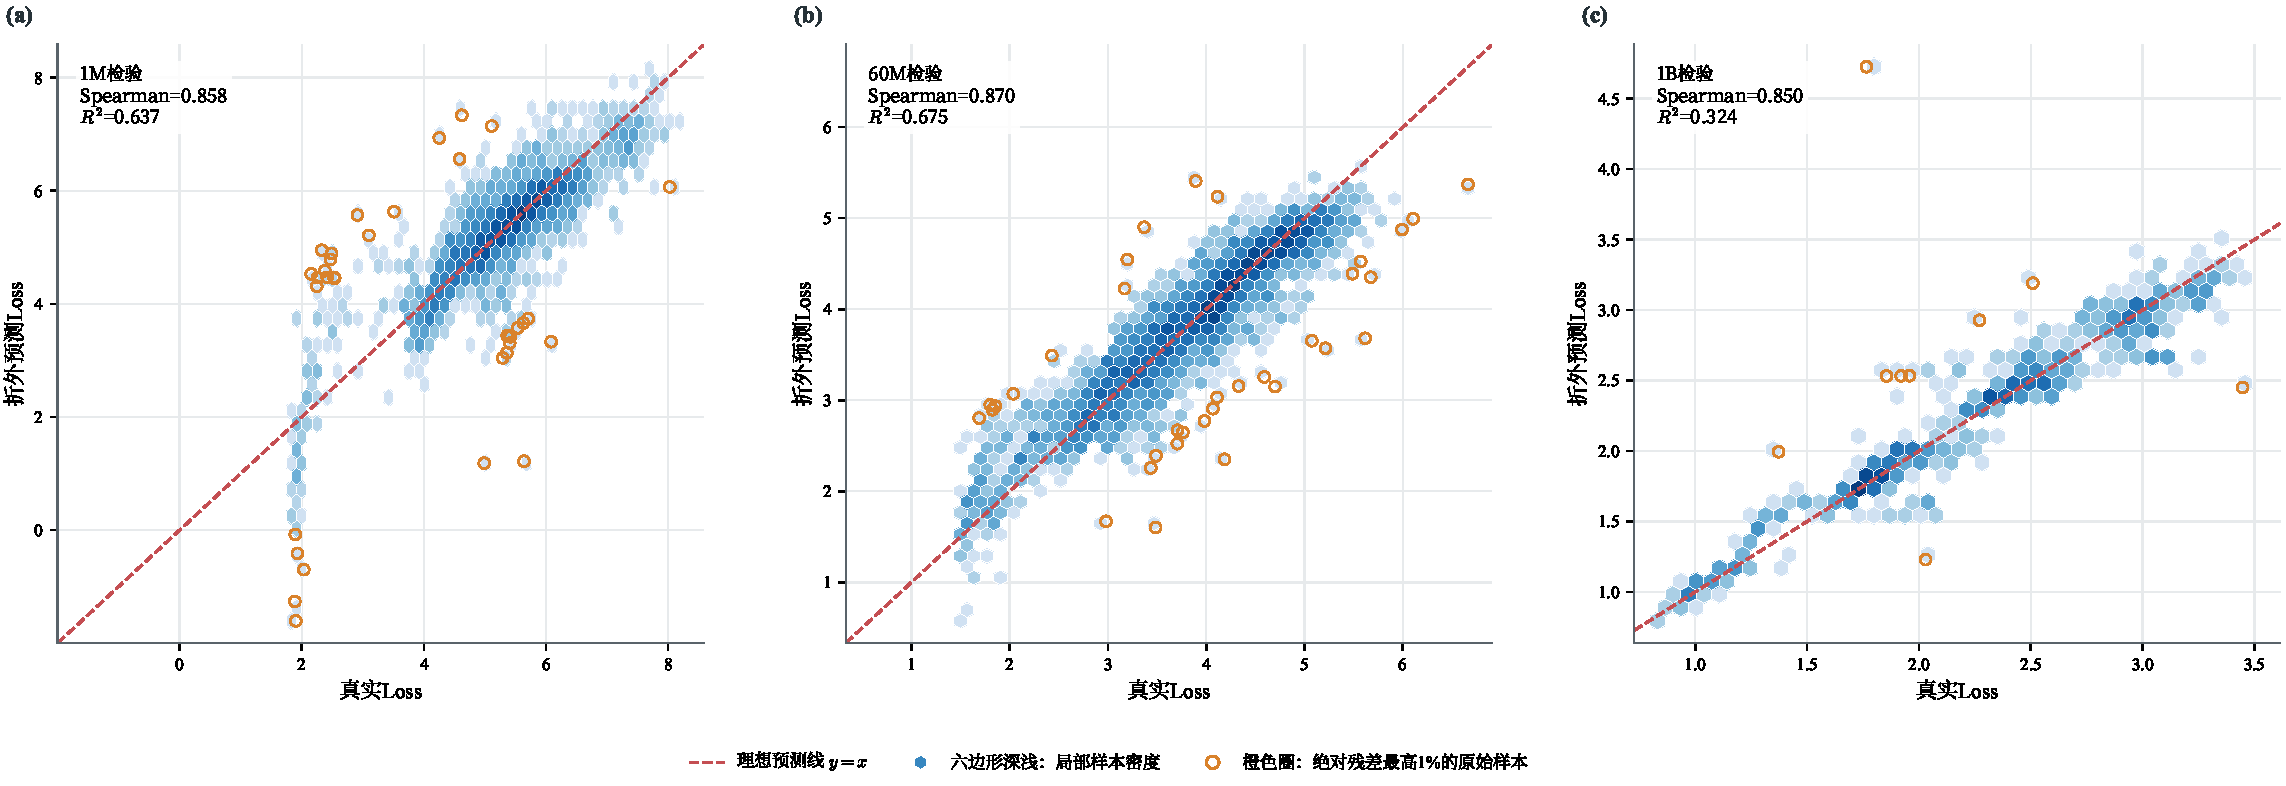
\includegraphics[width=0.98\linewidth]{images/no1/P1_F05_配比模型跨尺度验证.pdf}
\caption{二阶 Scheff\'e--Ridge 模型的跨尺度折外检验}
\label{fig:p1_f05}
\end{figure}

图~\ref{fig:p1_f06}进一步比较领域方向边际收益、两两交互和质量—收益排序。Ubuntu IRC 与 DeepMind Mathematics 的边际收益点估计分别约为 $3.665$ 和 $1.567$，对应 95\% 区间均位于正向 Loss 下降一侧；但其他领域的区间多跨越零，说明局部作用依赖起始配比。136 个领域对的交互中，大量符号在 bootstrap 下并不稳定，故本文只将其作为响应面结构诊断。

领域质量与边际收益的 Spearman、Kendall 系数分别为 $-0.1434$ 和 $-0.1048$，未呈现“质量越高、增配收益越大”的正向单调关系。由于推断域质量本身经过均值回退，且该相关尚无对应区间，结果只能说明静态质量不能代替配比实验，不足以证明二者完全无关。

\begin{figure}[htbp]
\centering
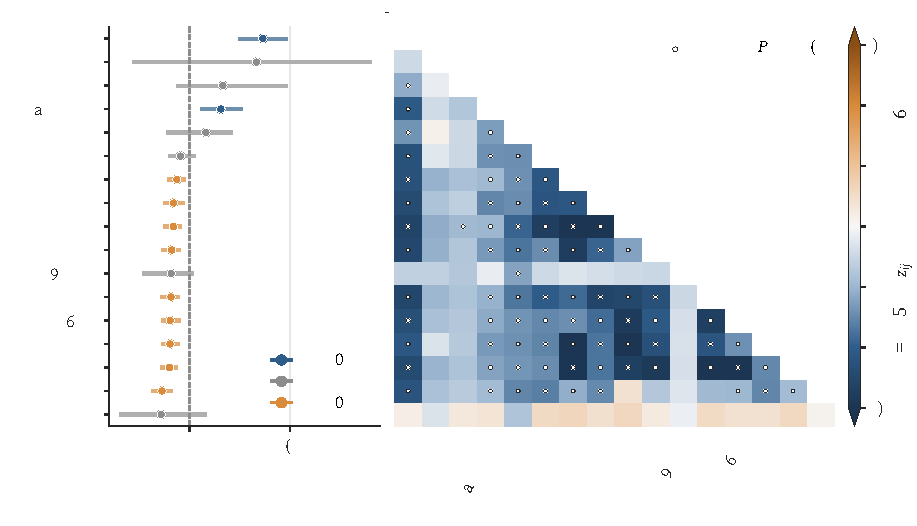
\includegraphics[width=0.98\linewidth]{images/no1/P1_F06_领域边际效应与交互网络.pdf}
\caption{领域边际效应、交互结构与质量—收益排序}
\label{fig:p1_f06}
\end{figure}

\subsubsection{支持域约束下的近优配比}

13 个验证域的 Loss 尺度不同。若直接求平均，高波动领域会主导目标。设训练集中第 $k$ 个验证域 Loss 的四分位距为 $s_k$，定义综合目标
\begin{equation}
J(\boldsymbol p)=\frac{1}{13}\sum_{k=1}^{13}
\frac{\widehat L_k(\boldsymbol p)}{s_k}.
\label{eq:p1_objective}
\end{equation}
四分位距只负责尺度归一化；各验证域在目标中保持等权。

响应面在训练配方附近最可靠。令 $u_i$ 为训练配比第 $i$ 个分量的 $99\%$ 分位，$\boldsymbol\sigma_p$ 为分量标准差，候选配比到训练集的标准化最近距离为 $d(\boldsymbol p)=\min_r\| (\boldsymbol p-\boldsymbol p_r^{\mathrm{train}})/\boldsymbol\sigma_p\|_2$。支持半径 $R$ 取训练点最近邻距离的 $99\%$ 分位，得到可行域
\begin{equation}
\mathcal P=\left\{
\boldsymbol p:
p_i\ge0,\quad \sum_i p_i=1,\quad p_i\le u_i,
\quad d(\boldsymbol p)\le R
\right\}.
\label{eq:p1_support_set}
\end{equation}
最终求解 $\min_{\boldsymbol p\in\mathcal P}J(\boldsymbol p)$。采用 30 个训练配比或其凸组合为起点进行 SLSQP 搜索，并用 10000 个独立随机可行点检查候选目标；在 200 次训练行 bootstrap 中重新拟合响应面并重新优化，用于评估份额不确定性。

表~\ref{tab:p1_optimal}列出点候选中占比最高的八个领域。USPTO backgrounds、PubMed abstracts、Stack Exchange 和 Europarl 合计占 $68.39\%$；但各领域 bootstrap 区间普遍较宽，多数领域存在落到零边界的可能，因此点配比不能脱离区间单独解读。其余九个领域在点候选中的合计占比为 $8.45\%$。

\begin{table}[htbp]
\centering
\small
\setlength{\tabcolsep}{5pt}
\caption{参考近优配比中占比最高的领域}
\label{tab:p1_optimal}
\begin{tabular}{lrrr}
\toprule
领域 & 点候选/\% & bootstrap 95\% 区间/\% & 零边界概率/\% \\
\midrule
USPTO backgrounds & 24.19 & [0.00, 55.61] & 38.0 \\
PubMed abstracts & 18.91 & [0.00, 53.09] & 71.0 \\
Stack Exchange & 14.91 & [0.00, 51.08] & 61.5 \\
Europarl & 10.38 & [0.00, 10.38] & 29.5 \\
Wikipedia (en) & 7.59 & [0.00, 25.85] & 50.5 \\
HackerNews & 7.15 & [0.00, 11.11] & 13.5 \\
PhilPapers & 4.88 & [0.00, 4.88] & 39.0 \\
Pile-CC & 3.55 & [0.00, 27.52] & 74.0 \\
\bottomrule
\end{tabular}
\end{table}

约束回代表明，点候选的比例和为 $1$，最大分量上界违反量仅为 $1.29\times10^{-14}$；支持距离和半径均为 $4.329687$，说明经验支持边界被激活。候选目标为 $4.7651$，优于 10000 个随机可行点中的最佳值 $5.2068$。然而，最佳五个可行起点的目标相对离散度仍为 $1.59\%$，未达到多起点一致性门槛。

图~\ref{fig:p1_f07}从组成空间投影、领域调整幅度和多起点解簇三个角度汇总求解结果。前两条 ILR--PCA 轴仅解释约 $18.05\%$ 的组成变异，二维投影不能代替原始 17 维约束检查；30 个起点中有 28 个得到可行结果，但只有 11 个同时具有正常终止标志。综合支持域边界、起点差异与 bootstrap 区间，本文将 $\boldsymbol p^\star$ 解释为当前响应面和实验范围支持的参考近优配比族，而不宣称其为真实训练空间中的唯一全局最优解。

\begin{figure}[htbp]
\centering
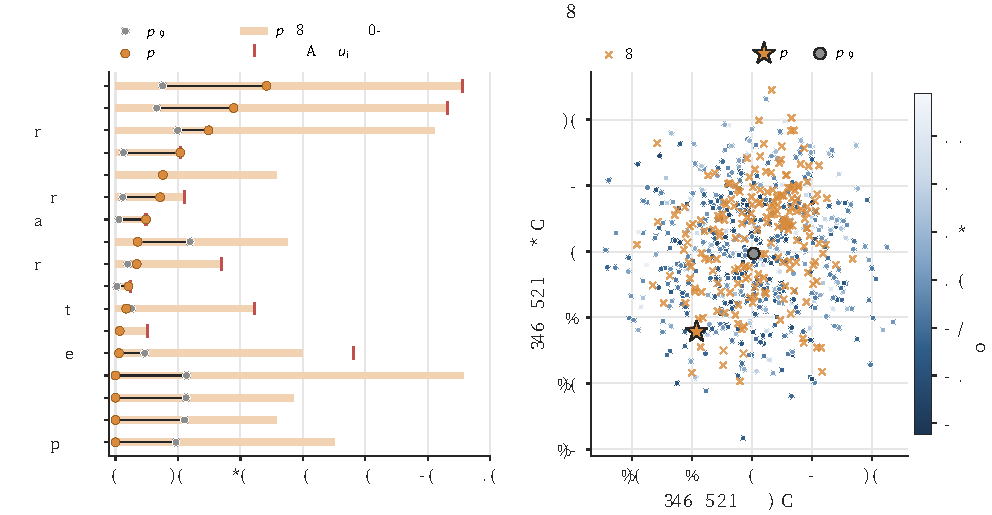
\includegraphics[width=0.98\linewidth]{images/no1/P1_F07_组成空间近优配比与不确定性.pdf}
\caption{组成空间中的参考近优配比及其不确定性}
\label{fig:p1_f07}
\end{figure}

\subsection{敏感性、适用边界与本问输出}

\subsubsection{近优配比的参数敏感性}

为区分“响应面正则强度”与“经验支持域定义”对解的影响，本文分别将支持半径和逐域份额上界的分位数由基准 $99\%$ 调整为 $95\%$、$97.5\%$，并将 Ridge 正则强度调整为 $0.5\alpha^*$ 和 $2\alpha^*$。所有情景均重新执行 30 起点约束优化，而非在基准解附近作线性近似。

图~\ref{fig:p1_f10}(a)显示，收紧支持半径至 $95\%$ 时，基准响应面目标上升 $2.61\%$，配比的 $L_1$ 变化为 $20.12$ 个百分点；将份额上界收紧至 $95\%$ 时，两者分别达到 $3.41\%$ 和 $61.42$ 个百分点。相比之下，$0.5\alpha^*$ 与 $2\alpha^*$ 仅使基准目标增加 $0.006\%$ 和 $0.014\%$，配比变化分别为 $2.77$ 和 $3.93$ 个百分点。图~\ref{fig:p1_f10}(b)进一步表明，约束收紧主要在生物医学全文、生医摘要、专利背景等领域之间重新分配份额，而正则强度扰动下 17 域变化均小于 1 个百分点。

\begin{figure}[htbp]
\centering
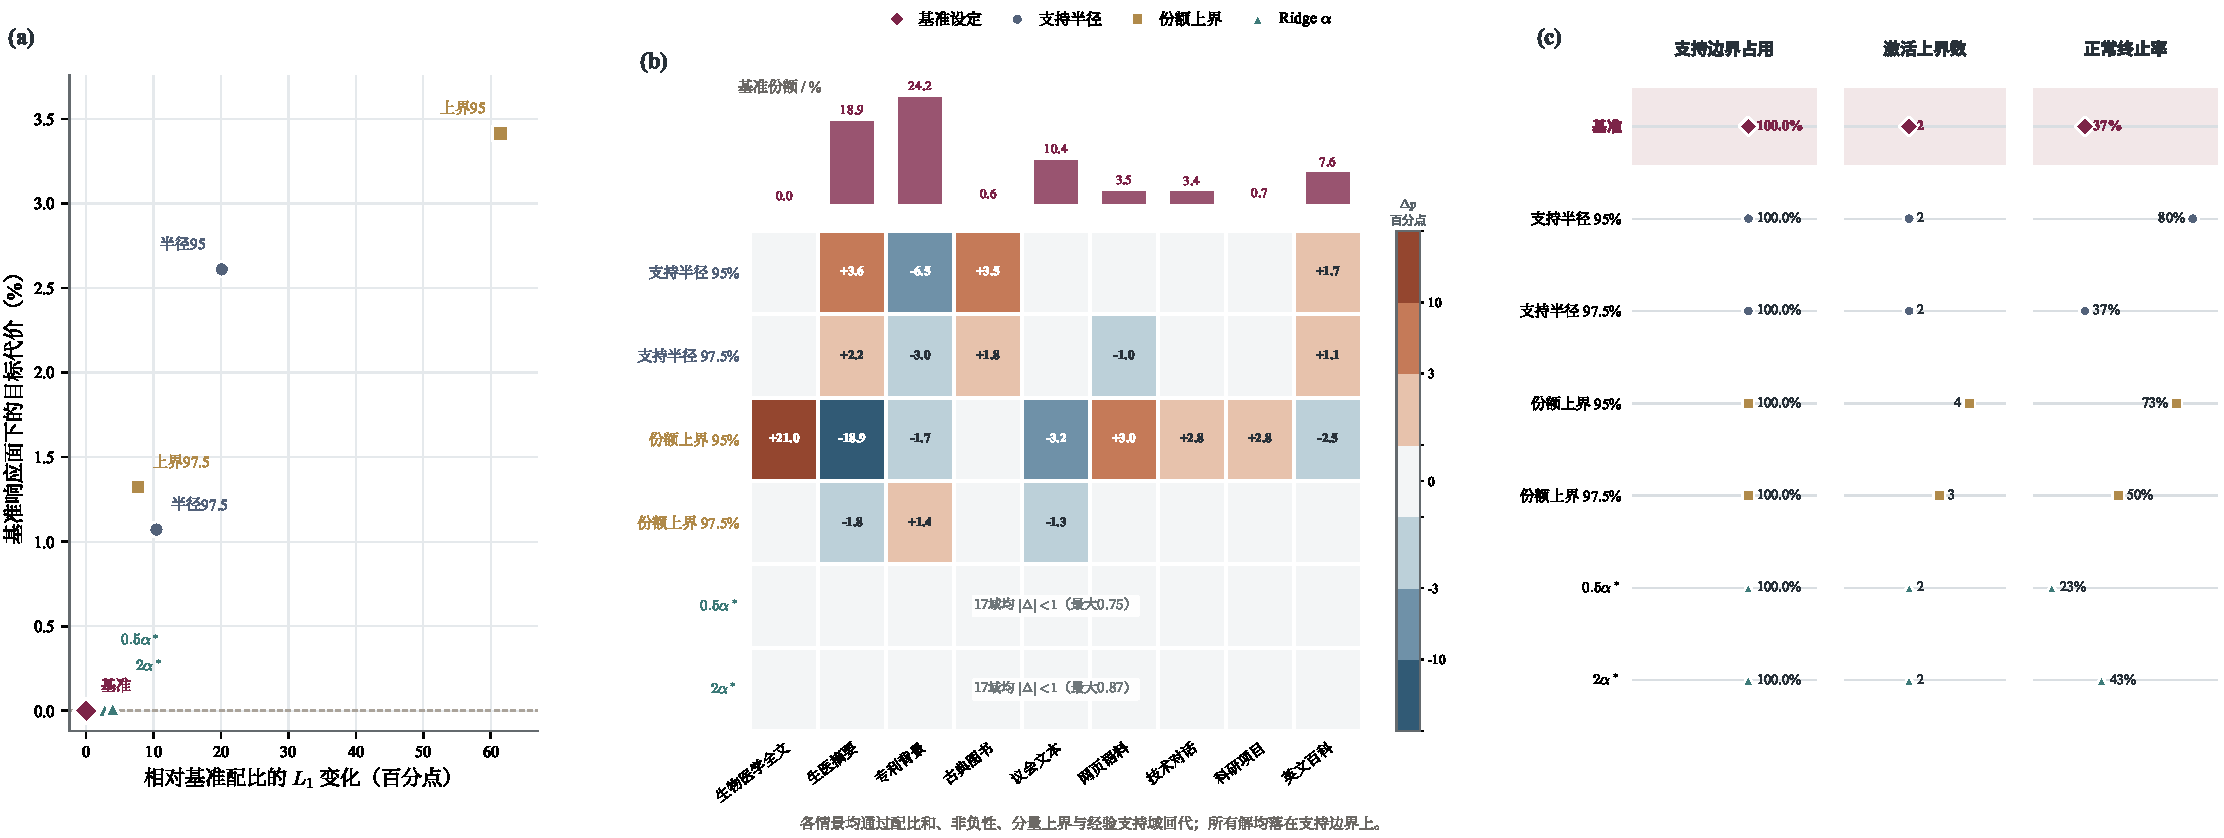
\includegraphics[width=0.99\linewidth]{images/no1/P1_F10_近优配比参数敏感性.pdf}
\caption{近优配比对支持域、份额上界与正则强度的敏感性}
\label{fig:p1_f10}
\end{figure}

七个情景的最优解均落在各自支持边界上，且至少 $28/30$ 个起点可得到可行解；正常终止率则在 $23\%$--$80\%$ 之间。由此可见，正则强度附近的扰动不会实质改变结论，而支持域和份额上界会明显改变点配比。该结果再次支持将 $\boldsymbol p^\star$ 报告为受经验边界约束的近优配比族，而不是唯一且可无条件外推的最优解。

综上，质量模型在统一 22 项异构信号的同时保留了块间冲突，七域质量和扩展集诊断可用于描述领域质量结构；但推断映射不足以支持 11 个领域的细粒度质量排序。二阶 Scheff\'e--Ridge 响应面在 1M、60M 和 1B 实测数据上保持了较好的配比排序能力，局部替换分析进一步说明领域收益依赖参照配方。近优搜索对正则强度较稳健，却明显受支持边界、份额上界和局部解簇影响。

本问向问题二传递的是“可追溯数据属性及其证据边界”，而非无条件的最优配方。具体接口见表~\ref{tab:p1_interface}。其中，$\boldsymbol p_{\mathrm{ref}}$ 是由训练配比样本计算的中性锚点，$\boldsymbol p^\star$ 则是受当前支持域约束的候选近优方案。由于配比改善量在 A、B 两套实验间没有绝对尺度校准，后续主模型优先使用 $\boldsymbol p_{\mathrm{ref}}$，并将 $\boldsymbol p^\star$ 保留为配比迁移的敏感性情景。

\begin{table}[htbp]
\centering
\small
\setlength{\tabcolsep}{5pt}
\caption{问题一向问题二传递的冻结接口}
\label{tab:p1_interface}
\begin{tabular}{p{0.22\linewidth}p{0.36\linewidth}p{0.32\linewidth}}
\toprule
接口 & 含义 & 后续用法 \\
\midrule
$\boldsymbol q$ & $17$ 域质量向量及映射置信边界 & 构造配比加权质量 \\
$\boldsymbol p_{\mathrm{ref}}$ & 训练配比样本的平均组成 & 主标度律的固定配比锚点 \\
$J(\boldsymbol p),R(\boldsymbol p)$ & 标准化综合 Loss 及相对配比响应 & 配比迁移方向与物理门槛检验 \\
$\boldsymbol p^\star$ & 支持域内的参考近优配比族 & 候选方案与敏感性分析 \\
\bottomrule
\end{tabular}
\end{table}


\section{问题二模型的建立与求解}
\label{sec:problem2}

\subsection{问题分析与建模思路}

问题二在经典参数--数据标度律上引入数据质量，并检验问题一的领域配比规律能否迁移到附件 B 的绝对 Loss 尺度。决策变量包括模型参数量 $N$、训练 Token 数 $D$、质量水平 $Q_A\in[0,1]$ 和 $17$ 域配比 $\boldsymbol p$；本问输出验证集交叉熵损失模型，供问题三在算力约束下调用。

附件 A 与附件 B 的实验对象和响应尺度不同，不能直接联合回归。本文先由 B1 识别经典标度律，再由 B7 估计质量惩罚，并将问题一的质量向量、参考配比和归一化配比响应作为冻结输入。模型分为固定参考配比的主接口 $\widehat L_{\mathrm{main}}(N,D,Q_A\mid\boldsymbol p_{\mathrm{ref}})$ 与带配比迁移项的情景扩展；前者用于资源分析，后者仅在强度可识别且不违反不可约损失下界时才允许进入决策。

求解依次完成基础模型选择、质量修正选择、资源弹性与等价关系计算以及配比接口验收，并以留出误差、排序保持、bootstrap 稳定性和物理下界作为共同门槛。

\begin{center}
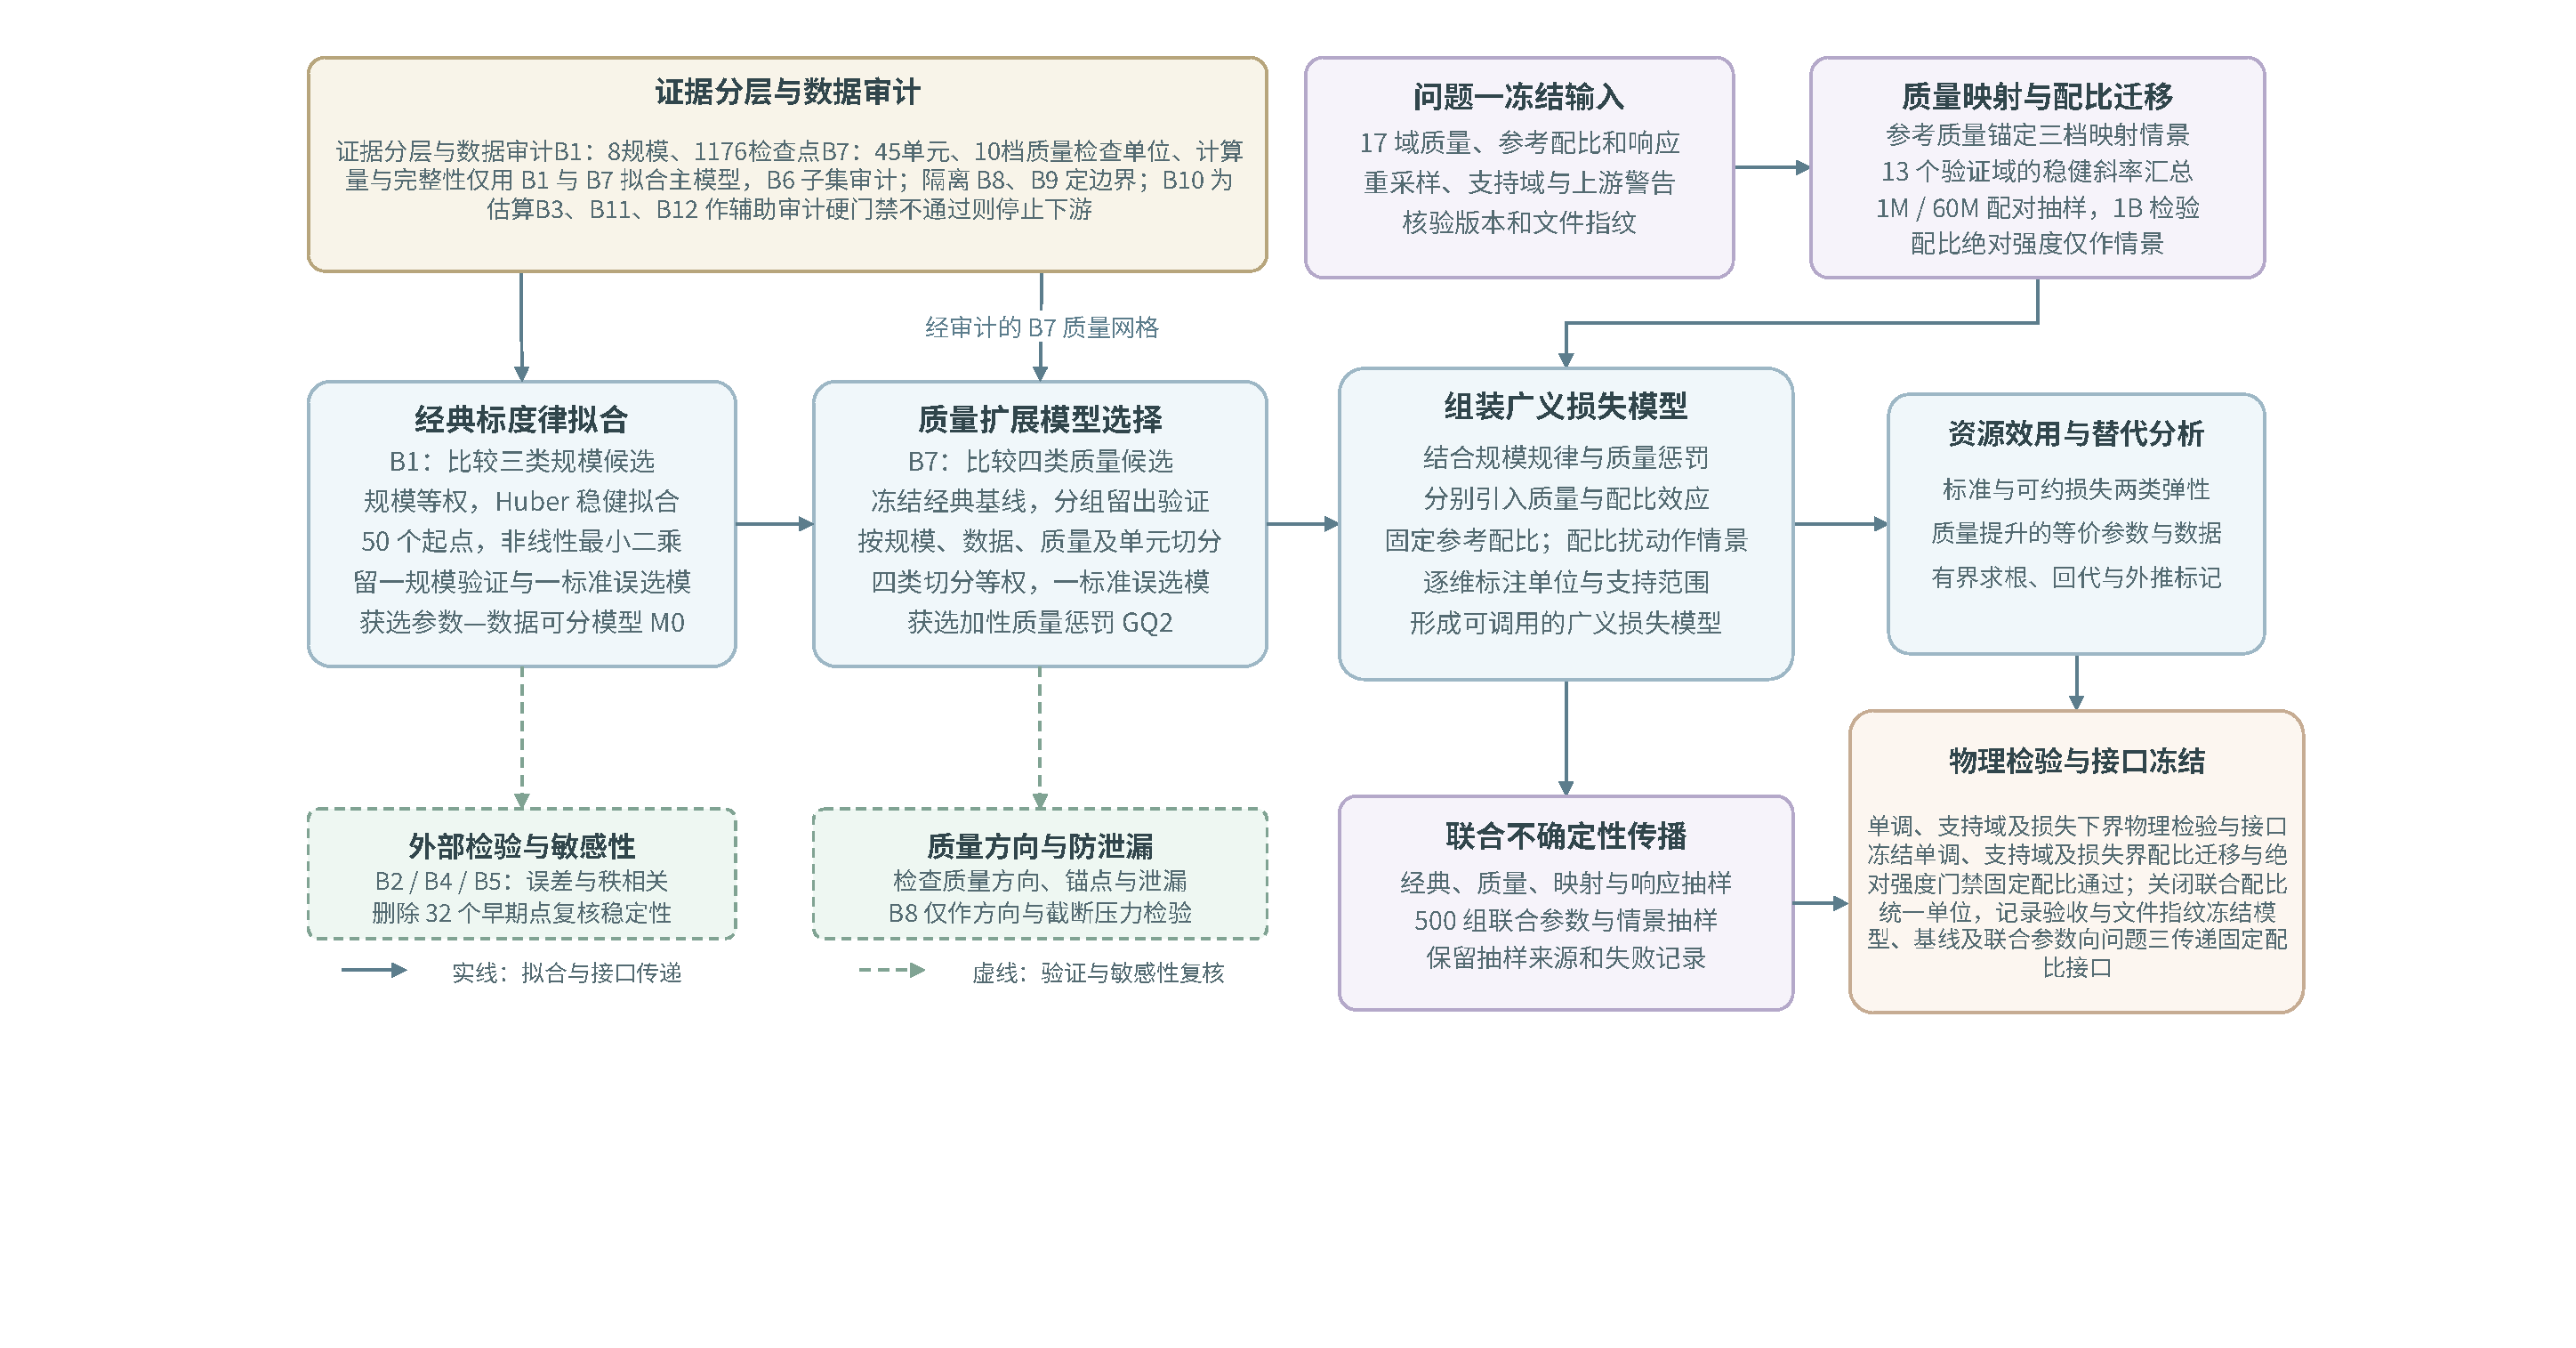
\includegraphics[width=0.96\linewidth]{images/no2/P2_F00_问题二求解流程图.pdf}
\captionof{figure}{问题二广义标度律的构建、检验与接口验收流程}
\label{fig:p2_solution_flow}
\end{center}

图~\ref{fig:p2_solution_flow} 以实线串联证据审计、模型拟合、资源分析与接口冻结，以虚线标出外部验证和敏感性复核；仅通过物理下界与稳定性门槛的接口才传入问题三。

\subsection{输入、数据与证据边界}

\subsubsection{数据审计与证据分层}

附件 B 的数据来源与可信程度不同，本文不作整表混合，而按表~\ref{tab:p2_evidence} 分配拟合、验证、压力测试和外推角色。参数量和训练数据量统一写为十亿尺度 $n=N/10^9$、$d=D/10^9$。

\begin{table}[!htbp]
\centering
\small
\setlength{\tabcolsep}{4pt}
\caption{附件 B 的证据分层与使用方式}
\label{tab:p2_evidence}
\begin{tabular}{p{0.13\linewidth}p{0.33\linewidth}p{0.43\linewidth}}
\toprule
数据源 & 数据性质 & 本问用途 \\
\midrule
B1 & $1176$ 条真实轨迹，覆盖 $8$ 个规模 & 拟合经典标度律并执行留一规模验证 \\
B2--B5 & 半合成轨迹、同源插值、跨族记录与文献数据 & 冻结参数后的外部一致性和排序检验 \\
B6--B7 & 分块质量实验，B6 为 B7 子集 & B6 作一致性核对，B7 的 $45\times10$ 网格拟合质量项 \\
B8 & 扩展质量网格，含反向响应和截断记录 & 仅作方向冲突与边界压力测试 \\
B9--B10 & 大模型规模信息与估算 Loss & 标记外推范围和量级，不增加独立观测证据 \\
B11--B12 & 模型族元数据与检查点索引 & 来源确认和轨迹完整性审计 \\
\bottomrule
\end{tabular}
\end{table}

据此记拟合集为 $\mathcal D_{\mathrm{fit}}=\{\mathrm{B1},\mathrm{B7}\}$，外部验证集主要由 B2--B5 构成，B8--B10 仅界定压力测试与外推边界。问题一的质量与配比结果同样以冻结接口输入，避免重复计算和跨体系信息泄漏。

\subsection{模型建立}

\subsubsection{经典参数—数据标度律模型}

以 $n=N/10^9$、$d=D/10^9$ 为无量纲规模，比较参数--数据可分幂律、总计算量幂律和带交互项幂律三类候选模型：
\begin{align}
M_0:\quad L_0(n,d)
&=E+A n^{-\alpha}+B d^{-\beta},
\label{eq:p2_classic_m0}\\
M_C:\quad L_C(n,d)
&=E_C+K_C(6nd)^{-\zeta},
\label{eq:p2_classic_mc}\\
M_{ND}:\quad L_{ND}(n,d)
&=E_{ND}+A_{ND}n^{-\alpha_{ND}}
+B_{ND}d^{-\beta_{ND}}+G(nd)^{-\xi}.
\label{eq:p2_classic_mnd}
\end{align}
其中，$E$ 类参数表示不可约损失，$6nd$ 为训练计算量代理，$G(nd)^{-\xi}$ 用于检验参数量与数据量的额外耦合。所有系数和衰减指数均约束为正，以保证规模增加时预测损失非增。最终依据 B1 的留一规模误差和简约性原则选型，B2--B5 仅用于冻结参数后的外部一致性检验。

\subsubsection{质量与配比的跨体系衔接}

设问题一输出的领域质量向量为 $\boldsymbol q=(q_1,\ldots,q_{17})^{\mathsf T}$，参考配比为 $\boldsymbol p_{\mathrm{ref}}$。任意配比 $\boldsymbol p$ 的加权质量及参考锚点定义为

\begin{equation}
Q_{\mathrm{base}}(\boldsymbol p)
=
\boldsymbol p^{\mathsf T}\boldsymbol q,
\qquad
Q_{\mathrm{ref}}
=
Q_{\mathrm{base}}(\boldsymbol p_{\mathrm{ref}})
=
0.5389559588,
\label{eq:p2_quality_bridge}
\end{equation}

其中 $Q_{\mathrm{base}}$ 是配比加权指标，不是直接观测的训练质量。为避免将问题一的配比 Loss 当作问题二的绝对 Loss，记 $\widehat{\ell}_k^A(\boldsymbol p)$ 为第 $k$ 个验证域的 Scheff\'e--Ridge 预测，$s_k$ 为其四分位距，定义

\begin{equation}
J(\boldsymbol p)
=
\frac{1}{13}
\sum_{k=1}^{13}
\frac{\widehat{\ell}_k^A(\boldsymbol p)}
{s_k},
\label{eq:p2_quality_bridge_J}
\end{equation}

并以参考配比中心化：

\begin{equation}
R(\boldsymbol p)
=
\frac{
J(\boldsymbol p)-J(\boldsymbol p_{\mathrm{ref}})
}
{
\operatorname{IQR}_{A4}[J(\boldsymbol p)]
},
\qquad
R(\boldsymbol p_{\mathrm{ref}})
=
0.
\label{eq:p2_mixture_bridge}
\end{equation}

分母取问题一 A4 样本上 $J(\boldsymbol p)$ 的四分位距，故 $R(\boldsymbol p)$ 只表达相对方向。由于两套质量尺度缺少独立校准实验，采用以 $Q_{\mathrm{ref}}$ 为锚点的情景映射

\begin{equation}
Q_{\mathrm{eff}}:=h_{s_Q}(Q_A)
=
\operatorname{clip}
\left[
Q_{\mathrm{ref}}
+
s_Q(Q_A-Q_{\mathrm{ref}}),
\varepsilon,
1
\right],
\qquad
s_Q\in\{0.5,1,1.5\},
\label{eq:p2_quality_map}
\end{equation}

其中 $s_Q=1$ 为主情景，$s_Q=0.5,1.5$ 用于敏感性分析，$\operatorname{clip}$ 保证有效质量落在可行区间。该映射和 $R(\boldsymbol p)$ 均为跨体系情景接口，不构成质量与配比已获联合实验识别的证据；主模型因此固定 $\boldsymbol p=\boldsymbol p_{\mathrm{ref}}$。

\subsubsection{固定配比主模型与配比迁移扩展}

记 B7 识别的质量惩罚为 $\Delta_Q(n,d,Q_{\mathrm{eff}})$。固定 $\boldsymbol p=\boldsymbol p_{\mathrm{ref}}$ 时，传给问题三的主模型为
\begin{equation}
\widehat L_{\mathrm{main}}(N,D,Q_A)
=L_0(n,d)+\Delta_Q\!\left(n,d,Q_{\mathrm{eff}}\right),
\qquad Q_{\mathrm{eff}}=h_{s_Q}(Q_A).
\label{eq:p2_main_interface}
\end{equation}
为检验问题一的相对配比响应能否进入 B 体系，再引入尺度迁移系数 $\lambda_0$ 和规模调整项 $(n/n_0)^{\delta_p}$，其中 $n_0$ 为 B7 参数规模中位数，得到情景扩展

\begin{equation}
\widehat L(N,D,Q_A,\boldsymbol p)
=
L_0(n,d)
+
\Delta_Q
\left(
n,d,Q_{\mathrm{eff}}
\right)
+
\lambda_0
\left(
\frac n{n_0}
\right)^{\delta_p}
R(\boldsymbol p),
\qquad
n=\frac{N}{10^9},
\quad
d=\frac{D}{10^9}.
\label{eq:p2_generalized}
\end{equation}

其中，$\lambda_0$ 连接 A、B 两套损失尺度，$\delta_p$ 描述配比效应随规模的变化。由于缺少四因素联合实验，非零 $\lambda_0$ 只作预设强度情景，不能视为可识别参数。主接口中 $R(\boldsymbol p_{\mathrm{ref}})=0$；进一步取 $Q_A=1,s_Q=1$ 时 $\Delta_Q=0$，模型恢复为 $L_0(n,d)$。超出 B 系列支持域的结果仅解释趋势，并保留外推标记。

\subsubsection{边际效用与资源等价指标构建}

令 $x\in\{N,D,Q_A\}$。局部边际效用取 $u_x=-\partial\widehat L/\partial x$；为消除资源量纲差异，进一步定义总损失弹性与可约损失弹性：

\begin{equation}
\epsilon_x=-\frac{x}{\widehat L}\frac{\partial\widehat L}{\partial x},
\qquad
\epsilon_x^{\mathrm{red}}=-\frac{x}{\widehat L-E}\frac{\partial\widehat L}{\partial x}
\quad(\widehat L>E).
\label{eq:p2_elasticity}
\end{equation}

前者衡量整体 Loss 的相对变化，后者以剩余可降低部分归一化，二者不混用。在固定参考配比且 $\lambda_0=0$ 的主情景下，GQ2 质量项为 $\Delta_Q=c_Q[1-h_{s_Q}(Q_A)]^{\nu_Q}$；映射未触及截断边界时，有

\begin{equation}
\frac{\partial\widehat L}{\partial N}
=
-\frac{\alpha A n^{-\alpha}}{N},
\qquad
\frac{\partial\widehat L}{\partial D}
=
-\frac{\beta B d^{-\beta}}{D},
\qquad
\frac{\partial\widehat L}{\partial Q_A}
=
-c_Q\nu_Q
[1-h_{s_Q}(Q_A)]^{\nu_Q-1}s_Q .
\label{eq:p2_derivatives}
\end{equation}

在等损失条件 $\mathrm d\widehat L=0$ 下，一阶 Taylor 展开给出质量提升的局部资源等价关系：

\begin{equation}
\Delta\log N
\simeq
\frac{
\partial\widehat L/\partial Q_A
}
{
N\,\partial\widehat L/\partial N
}
\Delta Q_A,
\qquad
\Delta\log D
\simeq
\frac{
\partial\widehat L/\partial Q_A
}
{
D\,\partial\widehat L/\partial D
}
\Delta Q_A.
\label{eq:p2_local_equivalence}
\end{equation}

对于较大质量变化，改用有限变化方程
\begin{align}
\widehat L(N',D,Q_A,\boldsymbol p_{\mathrm{ref}})
&=\widehat L(N,D,Q_A+\Delta Q_A,\boldsymbol p_{\mathrm{ref}}),\nonumber\\
\widehat L(N,D',Q_A,\boldsymbol p_{\mathrm{ref}})
&=\widehat L(N,D,Q_A+\Delta Q_A,\boldsymbol p_{\mathrm{ref}})
\label{eq:p2_finite_equivalence}
\end{align}
分别求得参数等价相对增幅 $r_N=N'/N-1$ 和数据等价相对增幅 $r_D=D'/D-1$。

上述等价量只比较模型预测的 Loss 变化，不表示计算成本、训练时间或经济成本相同。

\subsection{模型求解}

\subsubsection{经典标度律与质量修正模型参数估计}

不同模型层的数据来源和证据强度不同，故采用分阶段估计而不作四因素联合拟合。B1 拟合中以模型规模为聚类单位赋予等权重，使用 Huber 稳健非线性最小二乘和对数参数化 $\theta=\exp(\eta)$，并以拉丁超立方多起点降低初值影响。

模型评价按参数规模整体留一；当候选误差接近时，依照 one-SE 原则选择结构更简单者。验证结果见表~\ref{tab:p2_classic_cv}。

\begin{table}[!htbp]
\centering
\caption{经典标度律的留一模型规模验证结果}
\label{tab:p2_classic_cv}
\begin{tabular}{lrr}
\toprule
候选模型 & RMSE & 归一化 RMSE \\
\midrule
$M_0$ & 0.000147 & 0.000374 \\
$M_C$ & 0.084910 & 0.216303 \\
$M_{ND}$ & 0.000148 & 0.000376 \\
\bottomrule
\end{tabular}
\end{table}

实验结果表明，参数—数据可分幂律模型 $M_0$ 的留一规模 RMSE 为 $0.000147$，归一化 RMSE 为 $0.000374$；带交互项模型 $M_{ND}$ 的对应指标分别为 $0.000148$ 和 $0.000376$。虽然 $M_{ND}$ 增加了参数—数据交互项，但其验证误差并未降低，说明在当前 B1 数据范围内，额外交互结构未提供额外预测能力。因此，根据 one-SE 原则，选择结构更简洁的 $M_0$ 作为基础标度律模型。

\begin{figure}[!htbp]
\centering
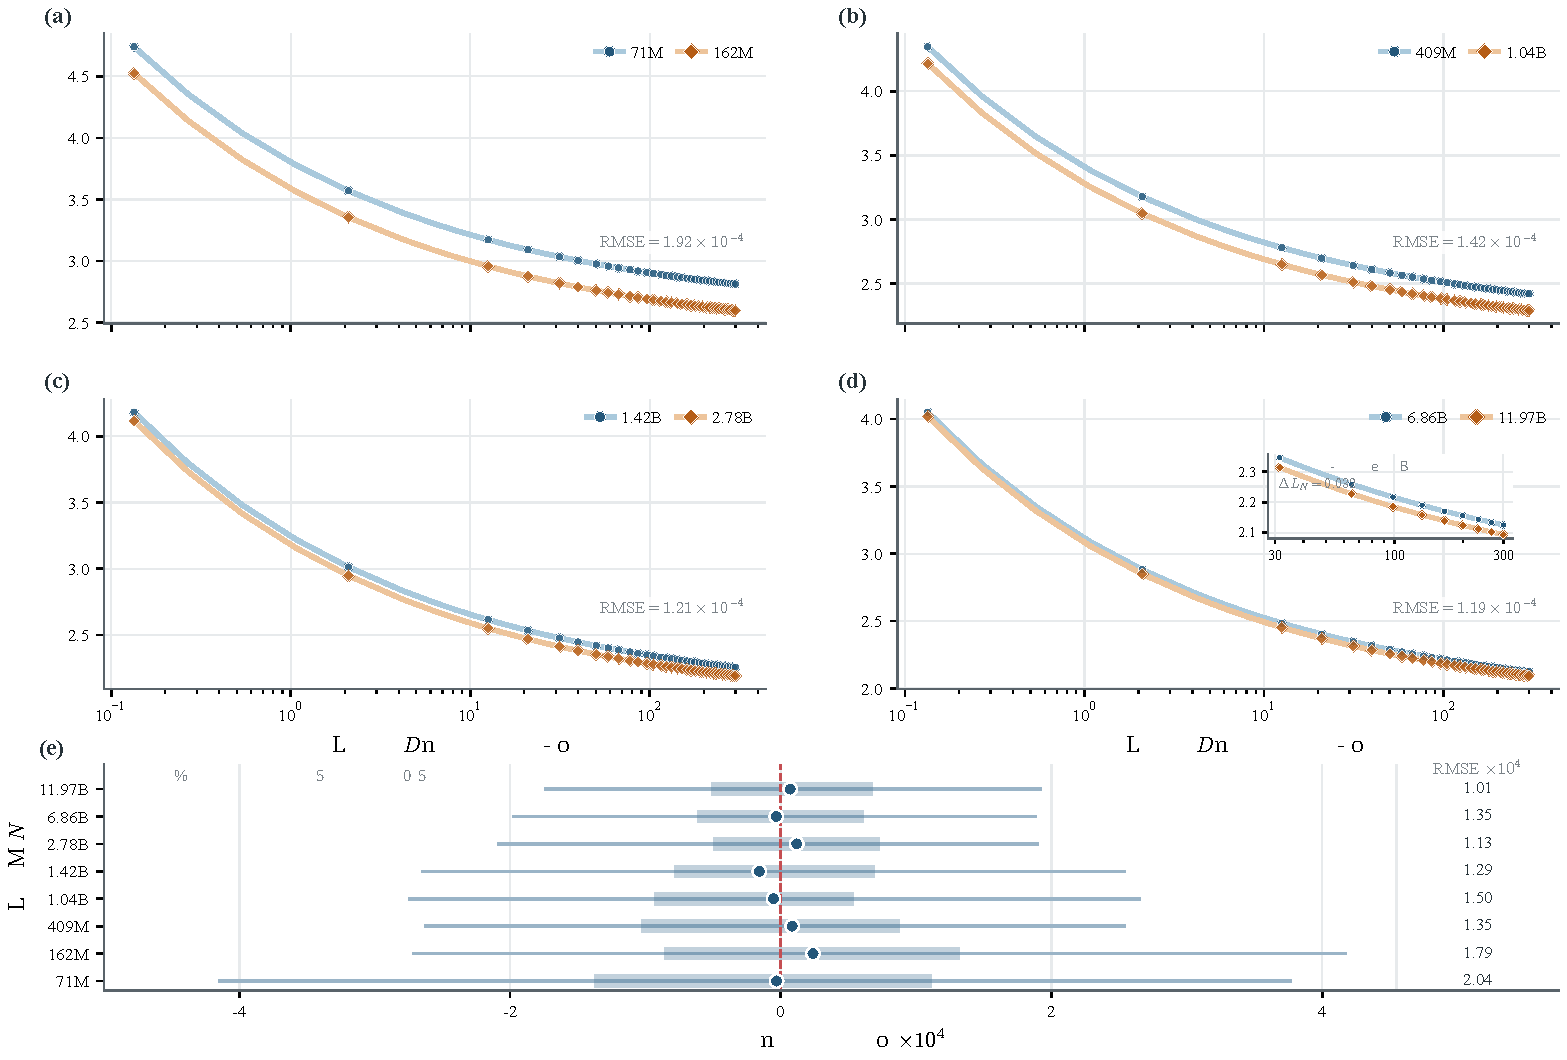
\includegraphics[width=0.98\linewidth]{images/no2/P2R_F01_经典标度律拟合与数据坍缩.pdf}
\caption{经典标度律在八种参数规模下的局部拟合与残差诊断}
\label{fig:p2_classic_fit}
\end{figure}

图~\ref{fig:p2_classic_fit} 将八条 B1 训练轨迹按参数规模两两分组。四个局部子图中，深色散点为观测检查点，浅色曲线为 $M_0$ 拟合结果；底部区间图进一步汇总各规模的残差范围和 RMSE。拟合曲线能够追踪不同模型规模下损失随 Token 增加的衰减趋势，且各规模残差均围绕零值分布，与留一规模验证对 $M_0$ 的选择相一致。

固定 B1 参数后，以 B7 估计增量质量项 $\widehat L=L_0(n,d)+\Delta_Q(n,d,Q)$。验证分别按参数规模、数据规模、质量水平和 $(N,D)$ 单元成块留出，各切分等权；验证折不提供 $Q_B=1$ 基线，以避免信息泄漏。依据成块误差和 one-SE 原则选择 GQ2。

\begin{figure}[!htbp]
\centering
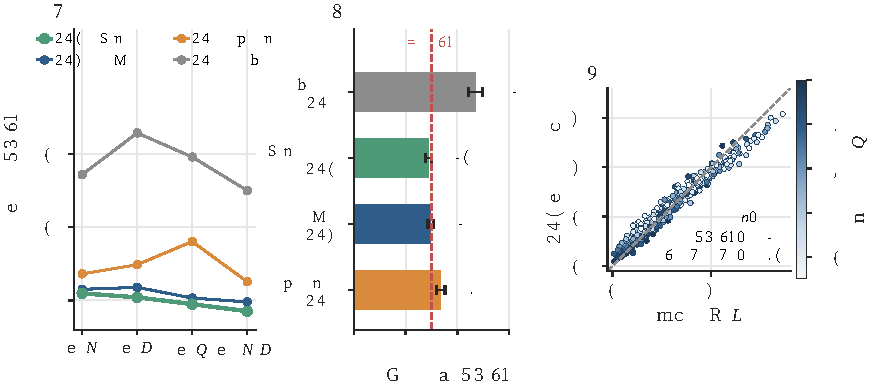
\includegraphics[width=0.98\linewidth]{images/no2/P2R_F02_质量模型成块交叉验证选择.pdf}
\caption{质量响应候选模型的成块交叉验证比较}
\label{fig:p2_quality_model_selection}
\end{figure}

图~\ref{fig:p2_quality_model_selection} 表明，GQ2 在 $69$ 个留出块上的等权 RMSE 为 $0.072$，较 GQ1 降低 $38.7\%$；其留数据规模、参数规模、质量水平和资源单元 RMSE 分别为 $0.073338$、$0.074643$、$0.071086$ 和 $0.068770$，优势并非由单一切分偶然造成。

\begin{center}
\centering
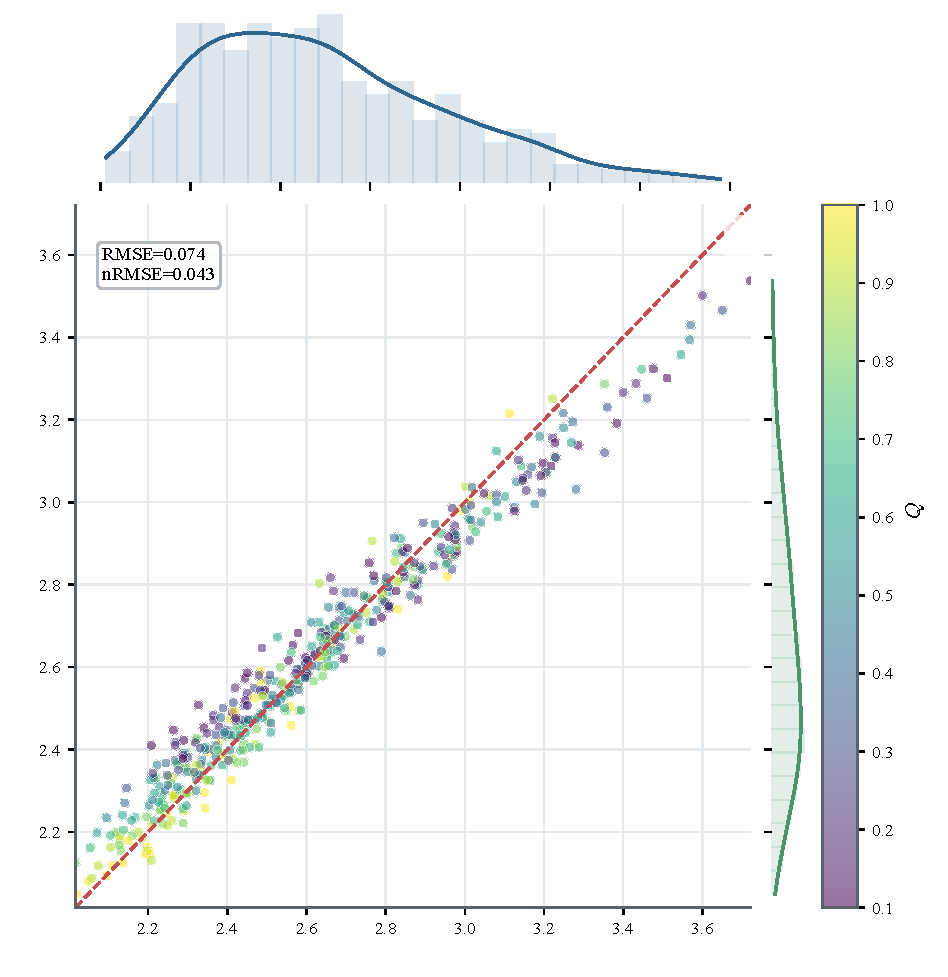
\includegraphics[width=0.74\linewidth]{images/no2/P2R_F03_GQ2预测观测边缘分布.pdf}
\captionof{figure}{GQ2 留资源单元验证的预测值与观测值联合分布}
\label{fig:p2_gq2_joint}
\end{center}

图~\ref{fig:p2_gq2_joint} 展示留 $(N,D)$ 资源单元验证中的逐点预测结果。中心散点按质量水平 $Q$ 着色，上方和右侧分别给出观测 Loss 与预测 Loss 的边缘分布。大部分样本沿 $1{:}1$ 线附近排列，说明模型能够捕捉主要变化趋势；高 Loss 尾部仍存在一定低估，因此后续外推仍需与支持域和压力测试结果结合解释。

随后，以 $(N,D)$ 资源单元作为 bootstrap 重采样簇，对质量修正参数进行 $500$ 次重复抽样，获得参数稳定性范围。在参考质量 $Q_{\mathrm{ref}}=0.538956$ 处，质量提高 $0.05$ 时预测 Loss 降低 $0.018071$，bootstrap $95\%$ 区间为 $[0.016565,\,0.019604]$；质量提高 $0.10$ 时预测 Loss 降低 $0.036164$，对应区间为 $[0.033208,\,0.039190]$。两组区间均未跨越零，说明当前实验支持域内的提质收益方向稳定。

问题一的配比信息不作为直接拟合参数，而通过冻结质量映射、Scheff\'e 响应和迁移抽样传播至广义模型。对 $1\mathrm{M}$、$60\mathrm{M}$ 和 $1\mathrm{B}$ 检验集，以稳健回归检验 $R(\boldsymbol p)$ 与标准化 Loss 的方向，并由前两个尺度的斜率比估计 $\delta_p$；因 A、B 体系缺少联合观测，非零配比强度只作预设情景。

最终得到基础标度律和质量修正参数估计结果：

\begin{equation}
\begin{aligned}
&(E,A,B,\alpha,\beta)
=
(1.6898,\,
0.35398,\,
1.24031,\,
0.339977,\,
0.279878),\\
&(c_Q,\nu_Q)
=
(0.36204,\,
0.990288).
\end{aligned}
\label{eq:p2_estimates}
\end{equation}

在 B7 数据的质量锚点 $Q_B=1$ 情景下，模型归一化 RMSE 为 $0.113203$。

B1 与 B7 分别估计经典项和质量项；B8--B10 不参与主模型选择，只承担压力测试和外推边界评估。

\begin{center}
\centering
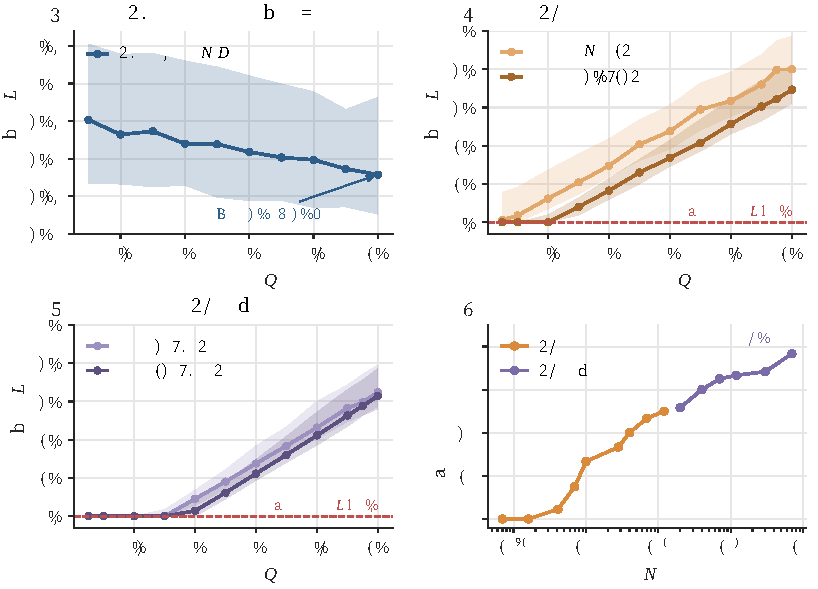
\includegraphics[width=0.99\linewidth]{images/no2/P2R_F04_B7与B8质量响应压力测试.pdf}
\captionof{figure}{B7 主质量网格与 B8 分规模压力测试}
\label{fig:p2_quality_stress}
\end{center}

图~\ref{fig:p2_quality_stress} 对上述证据分层给出直观检查。B7 主网格中 Loss 随质量提高而降低，方向与 GQ2 一致；B8 在部分大规模和远端区域出现方向反转及截断地板。地板记录比例随参数规模增大至 $38.3\%$，表明异常区域不宜反向影响主模型选择，而应作为外推边界和模型风险的压力测试证据。

\subsection{结果分析与模型验证}

\subsubsection{主模型响应与配比迁移方向}

在主身份映射情景 $s_Q=1$、$\boldsymbol p=\boldsymbol p_{\mathrm{ref}}$ 下，有 $Q_{\mathrm{eff}}=Q_A$ 且 $R(\boldsymbol p_{\mathrm{ref}})=0$，配比迁移项不参与主模型预测。因此，冻结标度律仅包含参数规模、训练数据规模和质量修正项：

\begin{equation}
\widehat L
=
1.689798
+
0.353980n^{-0.339977}
+
1.240306d^{-0.279878}
+
0.362040(1-Q)^{0.990288}.
\label{eq:p2_final_fixed_p}
\end{equation}

式~\eqref{eq:p2_final_fixed_p} 中，$E=1.689798$ 表示不可约损失水平。参数项 $0.353980n^{-0.339977}$ 与数据项 $1.240306d^{-0.279878}$ 分别描述两类规模扩张带来的损失下降；质量项 $0.362040(1-Q)^{0.990288}$ 表示训练数据质量偏离高质量状态时产生的额外损失。上述系数和指数均是当前实验支持域内的统计响应参数，而非跨所有模型族与训练策略均保持不变的物理常数。

在领域配比分析方面，问题一的归一化响应 $R(\boldsymbol p)$ 在 $1\mathrm{M}$、$60\mathrm{M}$ 与 $1\mathrm{B}$ 检验尺度下，与综合 Loss 的 Spearman 相关系数分别为 $0.812811$、$0.819749$ 和 $0.734158$。该结果说明配比响应在不同规模下保持一定方向一致性，但由于较大规模数据缺少 A、B 两体系之间的绝对 Loss 对齐信息，本文仅保留方向敏感性，不进行精确强度校准。

\begin{figure}[!htbp]
\centering
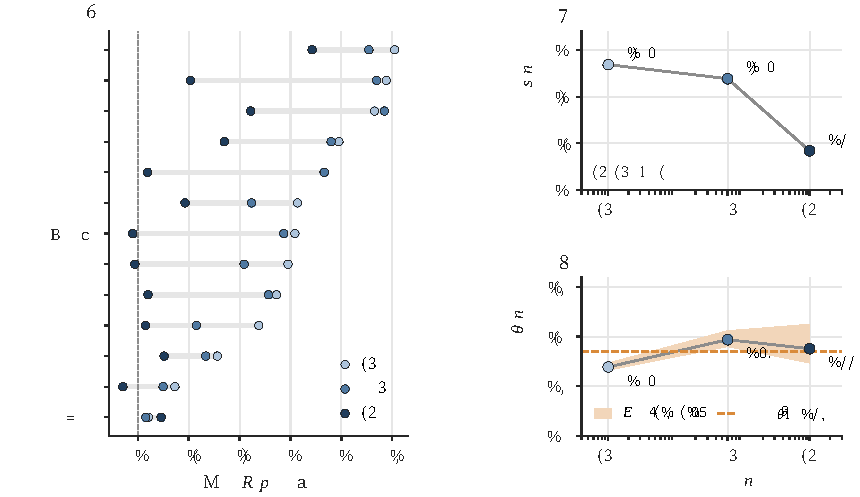
\includegraphics[width=0.96\linewidth]{images/no2/P2R_F05_配比效应跨尺度迁移.pdf}
\caption{配比响应的跨尺度迁移及其不确定性}
\label{fig:p2_mixture_transfer}
\end{figure}

图~\ref{fig:p2_mixture_transfer} 将各领域在三种检验尺度下的配比响应并置比较。$1\mathrm{M}$ 与 $60\mathrm{M}$ 下多数领域保持相同变化方向，而 $1\mathrm{B}$ 的综合响应仅为 $1\mathrm{M}$ 的 $31.2\%$，部分领域的 bootstrap 区间还出现跨零或方向反转。因此，配比结果可以支持跨尺度方向分析，却不足以支持固定强度的跨体系迁移。

进一步分析问题一 Scheff\'e 交互项，bootstrap 分类得到 $75$ 组互补关系和 $61$ 组不确定关系。负向二阶交互项表示相对于简单线性叠加，两个领域组合可能产生额外损失下降，而不确定关系不能解释为已验证的替代效应。候选方案 $\boldsymbol p^\star$ 的归一化响应为 $-2.289763$，bootstrap $95\%$ 区间为 $[-3.568433,\ 0.113031]$；由于该区间包含零，其仅作为敏感性情景，不视为稳定优于参考配比的决策结果。

\subsubsection{广义标度律地形与外推边界}

由式~\eqref{eq:p2_final_fixed_p} 可见，参数规模、数据规模与质量因素均通过衰减项影响预测损失，但其局部作用大小取决于当前资源状态。为同时观察规模效应、质量效应与外推边界，将连续预测曲面及其等 Loss 前沿绘于图~\ref{fig:p2_landscape}。

\begin{figure}[!htbp]
\centering
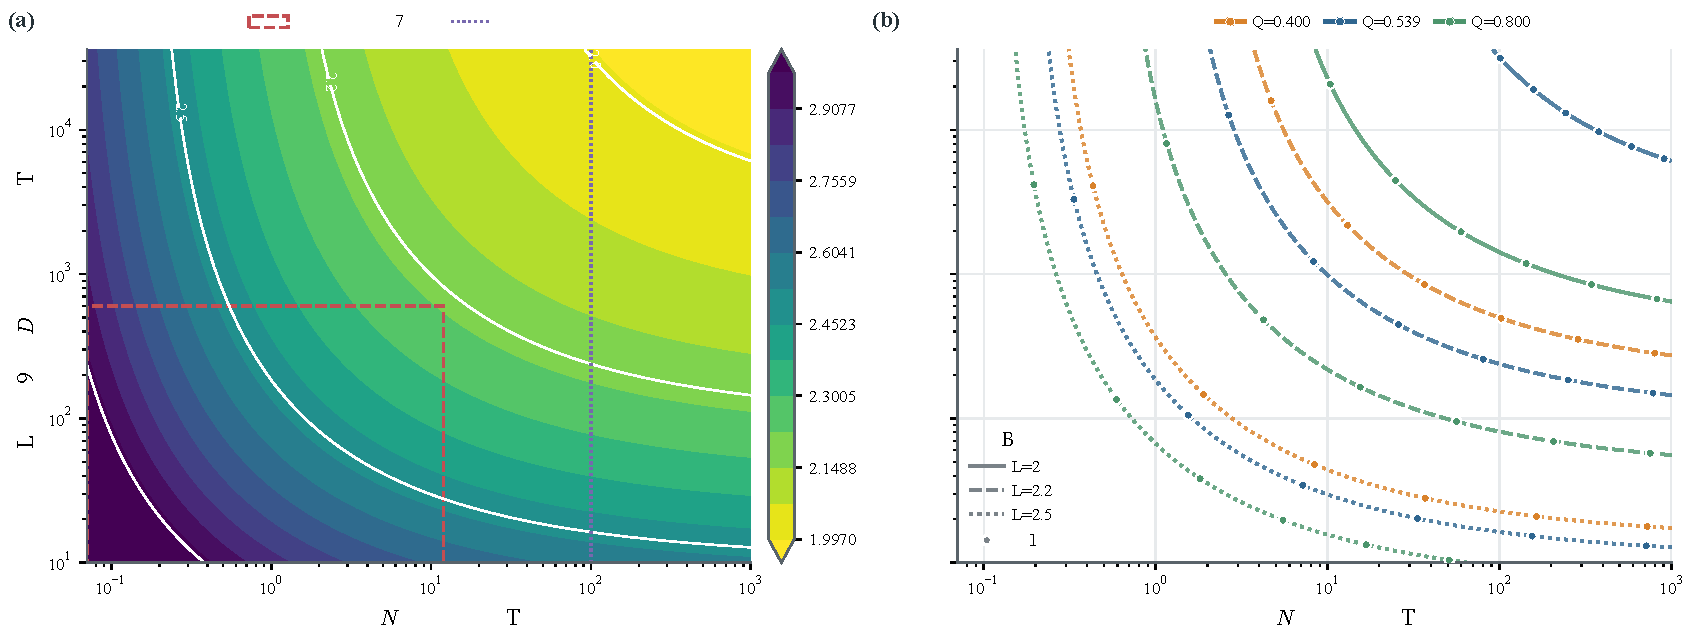
\includegraphics[width=0.98\linewidth]{images/no2/P2R_F06_广义标度律地形与等损失前沿.pdf}
\caption{固定参考配比下的广义标度律地形与等 Loss 前沿}
\label{fig:p2_landscape}
\end{figure}

图~\ref{fig:p2_landscape}(a) 标出 B1/B7 观测支持域与 B9 扩展起点，表明大规模结果在几何上已离开主拟合区域；图~\ref{fig:p2_landscape}(b) 显示，质量提高会使等 Loss 前沿系统向更低的参数量或 Token 量方向移动。图中圆点是从连续模型前沿上抽取的计算节点，而非新的原始观测，因此前沿仅用于资源关系解释，不能被误读为外推区域已获得实验验证。

\subsubsection{资源弹性与有限等价关系}

为比较不同资源在模型所处状态变化时的相对作用，首先计算参数、Token 和质量的标准总 Loss 弹性，并在 $27$ 个 $N$--$D$--$Q$ 网格状态上汇总其组成。

\begin{figure}[!htbp]
\centering
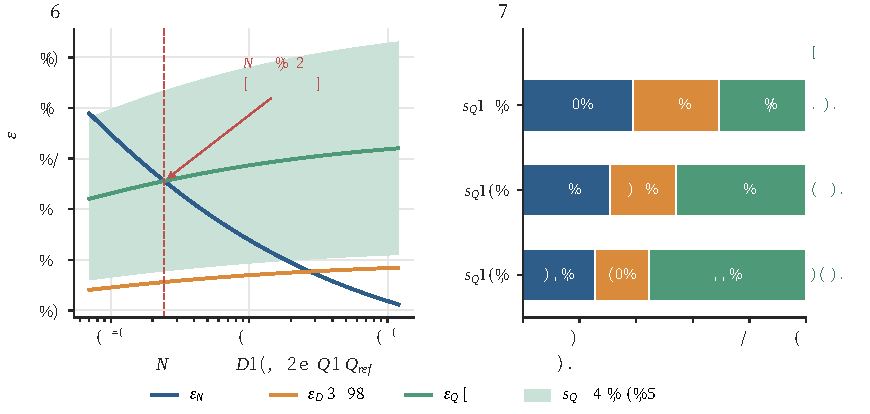
\includegraphics[width=0.96\linewidth]{images/no2/P2R_F07_资源弹性组成状态图.pdf}
\caption{固定参考配比下的资源弹性路径与主导结构迁移}
\label{fig:p2_elasticity}
\end{figure}

图~\ref{fig:p2_elasticity}(a) 在 $D=150\mathrm{B}$ 和参考质量下跟踪三类弹性随参数规模的连续变化；主情景中，质量弹性约在 $N=0.24\mathrm{B}$ 后超过参数弹性。图~\ref{fig:p2_elasticity}(b) 表明，当 $s_Q$ 从 $0.5$ 增加至 $1.5$ 时，质量平均弹性份额由 $30.8\%$ 增至 $55.5\%$，质量主导状态也由 $7/27$ 增至 $21/27$。因此，质量映射强度是资源主导结构的关键不确定性来源。

进一步以 B7 参数规模和数据规模的中位参考点为基准，取 $Q_A=0.538956$、$s_Q=1$、$\Delta Q_A=0.1$，代入式~\eqref{eq:p2_finite_equivalence} 求得资源等价关系。质量评分提高 $0.1$ 时，其损失下降效果分别等价于在原质量水平下将参数规模增加 $r_N=0.372985$，或将训练数据规模增加 $r_D=0.569474$，即约相当于参数扩张 $37.30\%$ 或数据扩张 $56.95\%$。

\begin{figure}[!htbp]
\centering
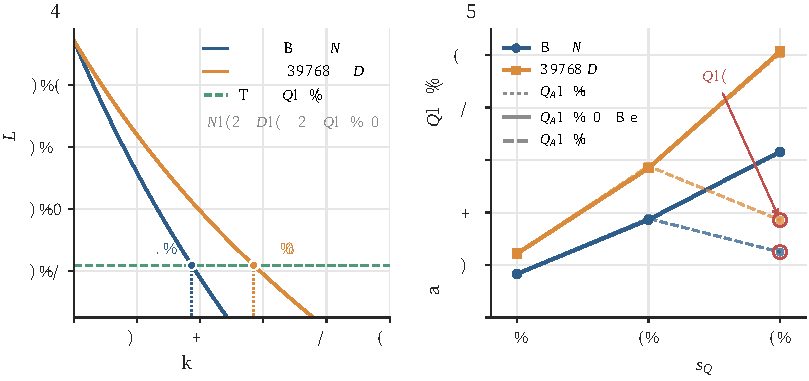
\includegraphics[width=0.95\linewidth]{images/no2/P2R_F08_质量提升的有限资源等价量.pdf}
\caption{质量提升 $0.10$ 的有限资源等价量及其情景变化}
\label{fig:p2_finite_equivalence}
\end{figure}

图~\ref{fig:p2_finite_equivalence}(a) 通过同一目标 Loss 下的两组交点直观展示 $37.30\%$ 和 $56.95\%$ 的有限等价增幅；图~\ref{fig:p2_finite_equivalence}(b) 利用 $18$ 个实际计算点展示结果随基线质量和 $s_Q$ 的变化。高质量且 $s_Q=1.5$ 时，质量映射触及 $Q=1$ 截断边界，因此等价增幅出现回落。该结果只表示模型空间中的性能等价，未计入提升数据质量的实际成本，不能直接解释为工程成本等价。

除标准总 Loss 弹性外，在 $\widehat L>E$ 条件下还可计算可约损失弹性，用于分析距离不可约极限较远区域的资源敏感性。两类弹性的归一化对象不同，不宜直接混用；同时，不同 $s_Q$ 会显著改变等价结果，故跨体系质量映射假设是解释结果的重要前提。

\subsection{敏感性、适用边界与本问输出}

\subsubsection{配比接口的物理门槛}

由于 A、B 两套实验体系中的损失量纲和实验条件不同，目前不存在能够直接识别 $\lambda_0$ 的共同绝对 Loss 实验，因此非零配比强度不能作为主模型中的自由拟合参数。在联合配比情景检查中，共有 $52$ 组预测出现 $\widehat L<E$，最低预测值为 $1.047781$，低于不可约项 $E=1.689798$。

\begin{figure}[!htbp]
\centering
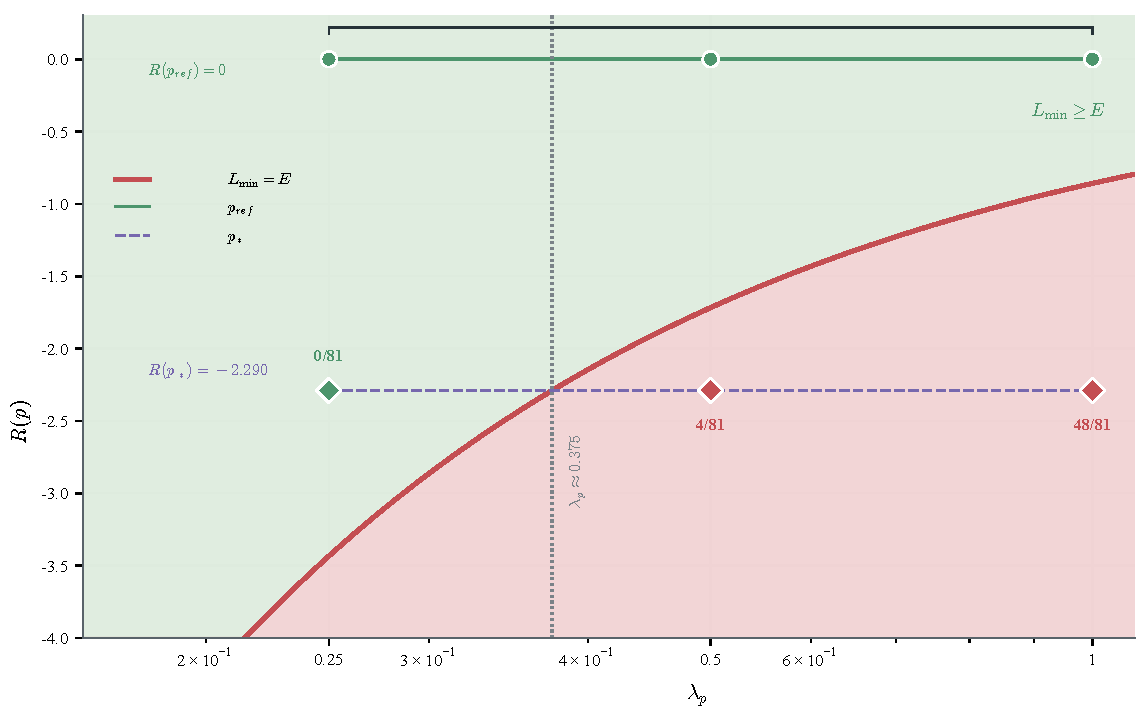
\includegraphics[width=0.90\linewidth]{images/no2/P2R_F09_配比接口物理门槛.pdf}
\caption{配比迁移强度与配比响应共同决定的物理可行域}
\label{fig:p2_mixture_gate}
\end{figure}

图~\ref{fig:p2_mixture_gate} 以 $\min\widehat L=E$ 为边界将情景空间分为物理可行区和阻断区。参考配比满足 $R(\boldsymbol p_{\mathrm{ref}})=0$，在已检查强度范围内始终不跌破不可约损失；近优配比情景在 $\lambda_0=0.5$ 和 $1$ 时分别有 $4/81$ 和 $48/81$ 个网格点违规。图中 $\lambda_0\approx0.375$ 是当前模型情景下的解析门槛，而非由跨体系共同实验识别得到的经验常数。

上述结果说明当前非零配比迁移情景可能进入基础标度律不支持的预测区域。因此，中心标度律模型和固定配比接口通过验收，而联合配比接口暂不具备决策使用条件。后续资源配置分析仅采用 $\boldsymbol p=\boldsymbol p_{\mathrm{ref}}$、$\lambda_0=0$ 的主接口。

综合模型选择、质量分块验证和配比物理门槛检查，本问形成表~\ref{tab:p2_interface} 所示的分层输出；第~\ref{sec:problem3} 节只在 $\boldsymbol p=\boldsymbol p_{\mathrm{ref}}$、$\lambda_0=0$ 下优化 $N$、$D$ 和 $Q_A$。

\begin{table}[!htbp]
\centering
\small
\setlength{\tabcolsep}{4pt}
\caption{问题二向问题三传递的冻结接口}
\label{tab:p2_interface}
\begin{tabular}{p{0.25\linewidth}p{0.34\linewidth}p{0.31\linewidth}}
\toprule
接口 & 冻结内容 & 决策状态 \\
\midrule
基础标度律 & $E,A,B,\alpha,\beta$ 及 $n=N/10^9,d=D/10^9$ & 通过，进入问题三 \\
质量修正 & GQ2 的 $c_Q,\nu_Q$ 与 $Q_{\mathrm{eff}}=h_{s_Q}(Q_A)$ & 通过，$s_Q$ 作情景参数 \\
参考锚点 & $Q_{\mathrm{ref}}=0.5389559588$，$\boldsymbol p=\boldsymbol p_{\mathrm{ref}}$ & 通过，作为中心情景 \\
配比迁移 & $\lambda_0(n/n_0)^{\delta_p}R(\boldsymbol p)$ & 未通过，仅作敏感性分析 \\
支持域标记 & B1/B7 观测域、单分量外推和桥接缺口 & 随问题三每个方案一并传递 \\
\bottomrule
\end{tabular}
\end{table}

\subsubsection{外部验证、稳健性与适用边界}

图~\ref{fig:p2_external_validation} 汇总冻结经典标度律的跨来源预测。B2、B4 和 B5 分别代表半合成族外轨迹、跨模型族记录和公开文献数据；B10 的 Loss 来源于估算结果，因此只作量级对照，不增加独立观测证据。

\begin{center}
\centering
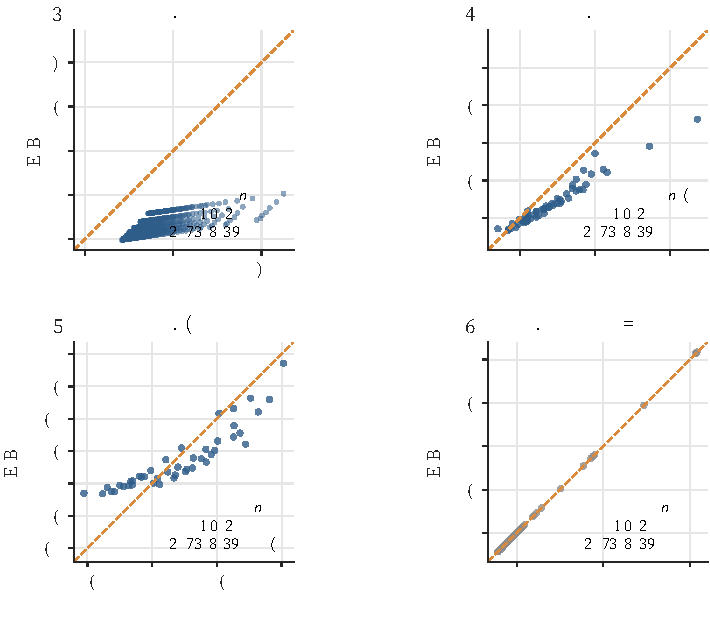
\includegraphics[width=0.66\linewidth]{images/no2/P2R_F10_经典标度律外部证据验证.pdf}
\captionof{figure}{冻结经典标度律的跨来源预测诊断}
\label{fig:p2_external_validation}
\end{center}

图~\ref{fig:p2_external_validation} 中，B2 的 RMSE 为 $1.243085$，存在明显绝对偏差；B4 与 B5 的 Spearman 相关系数分别为 $0.982982$ 和 $0.958808$；B10 虽接近 $1{:}1$ 线，但属于估算值。因此，跨来源分析只检验组内趋势和排序，不直接比较绝对 Loss。

剔除 B1 中 $D<2$（十亿 Token）的 $32$ 个早期检查点后，参数最大相对变化仅为 $0.052965\%$，表明估计稳定。B9 仅界定外推边界，B10 不能替代真实大模型训练验证；因此，超出 B1/B7 支持域的预测均保留外推标记，并结合验证证据谨慎解释。


\section{问题三模型的建立与求解}
\label{sec:problem3}

\subsection{问题分析与建模思路}

问题三在总算力约束下联合配置参数量、训练数据量和数据质量。经典标度律描述参数量与训练 Token 数对损失的幂律作用\cite{kaplan2020scaling,hoffmann2022compute}；本问进一步把质量提升和长文本注意力纳入统一预算，考察三类资源竞争及跨预算结构转移。

问题一给出 $17$ 个领域的参考配比 $\boldsymbol p_{\mathrm{ref}}$，问题二给出广义标度律。由于现有检验只支持固定配比接口，本问不再优化十七维配比，而令

\begin{equation}
\boldsymbol p=\boldsymbol p_{\mathrm{ref}},
\qquad
D_i=p_{\mathrm{ref},i}D,\quad i=1,\ldots,17.
\label{eq:p3_fixed_mixture}
\end{equation}

即先优化总 Token 数 $D$，再分解到各领域。决策量为 $N,D,Q_A$，预算 $C$、上下文 $L_{\mathrm{ctx}}$ 与质量成本 $g$ 为外生情景。利用损失关于 $D$ 严格递减的性质，可解析消去 $D$，再通过多起点精化、预算追踪和三维复核求解，并由 KKT 条件与配置弹性解释结构转移。

总体路线见图~\ref{fig:p3_solver_flow}：从前两问冻结接口出发，依次完成可行性判断、二维求解、三维复核、成本回代及 KKT 与抽样检验，再将验收通过的情景发布给问题四；具体计算顺序见算法~\ref{alg:p3_solver}。

\begin{figure}[H]
\centering
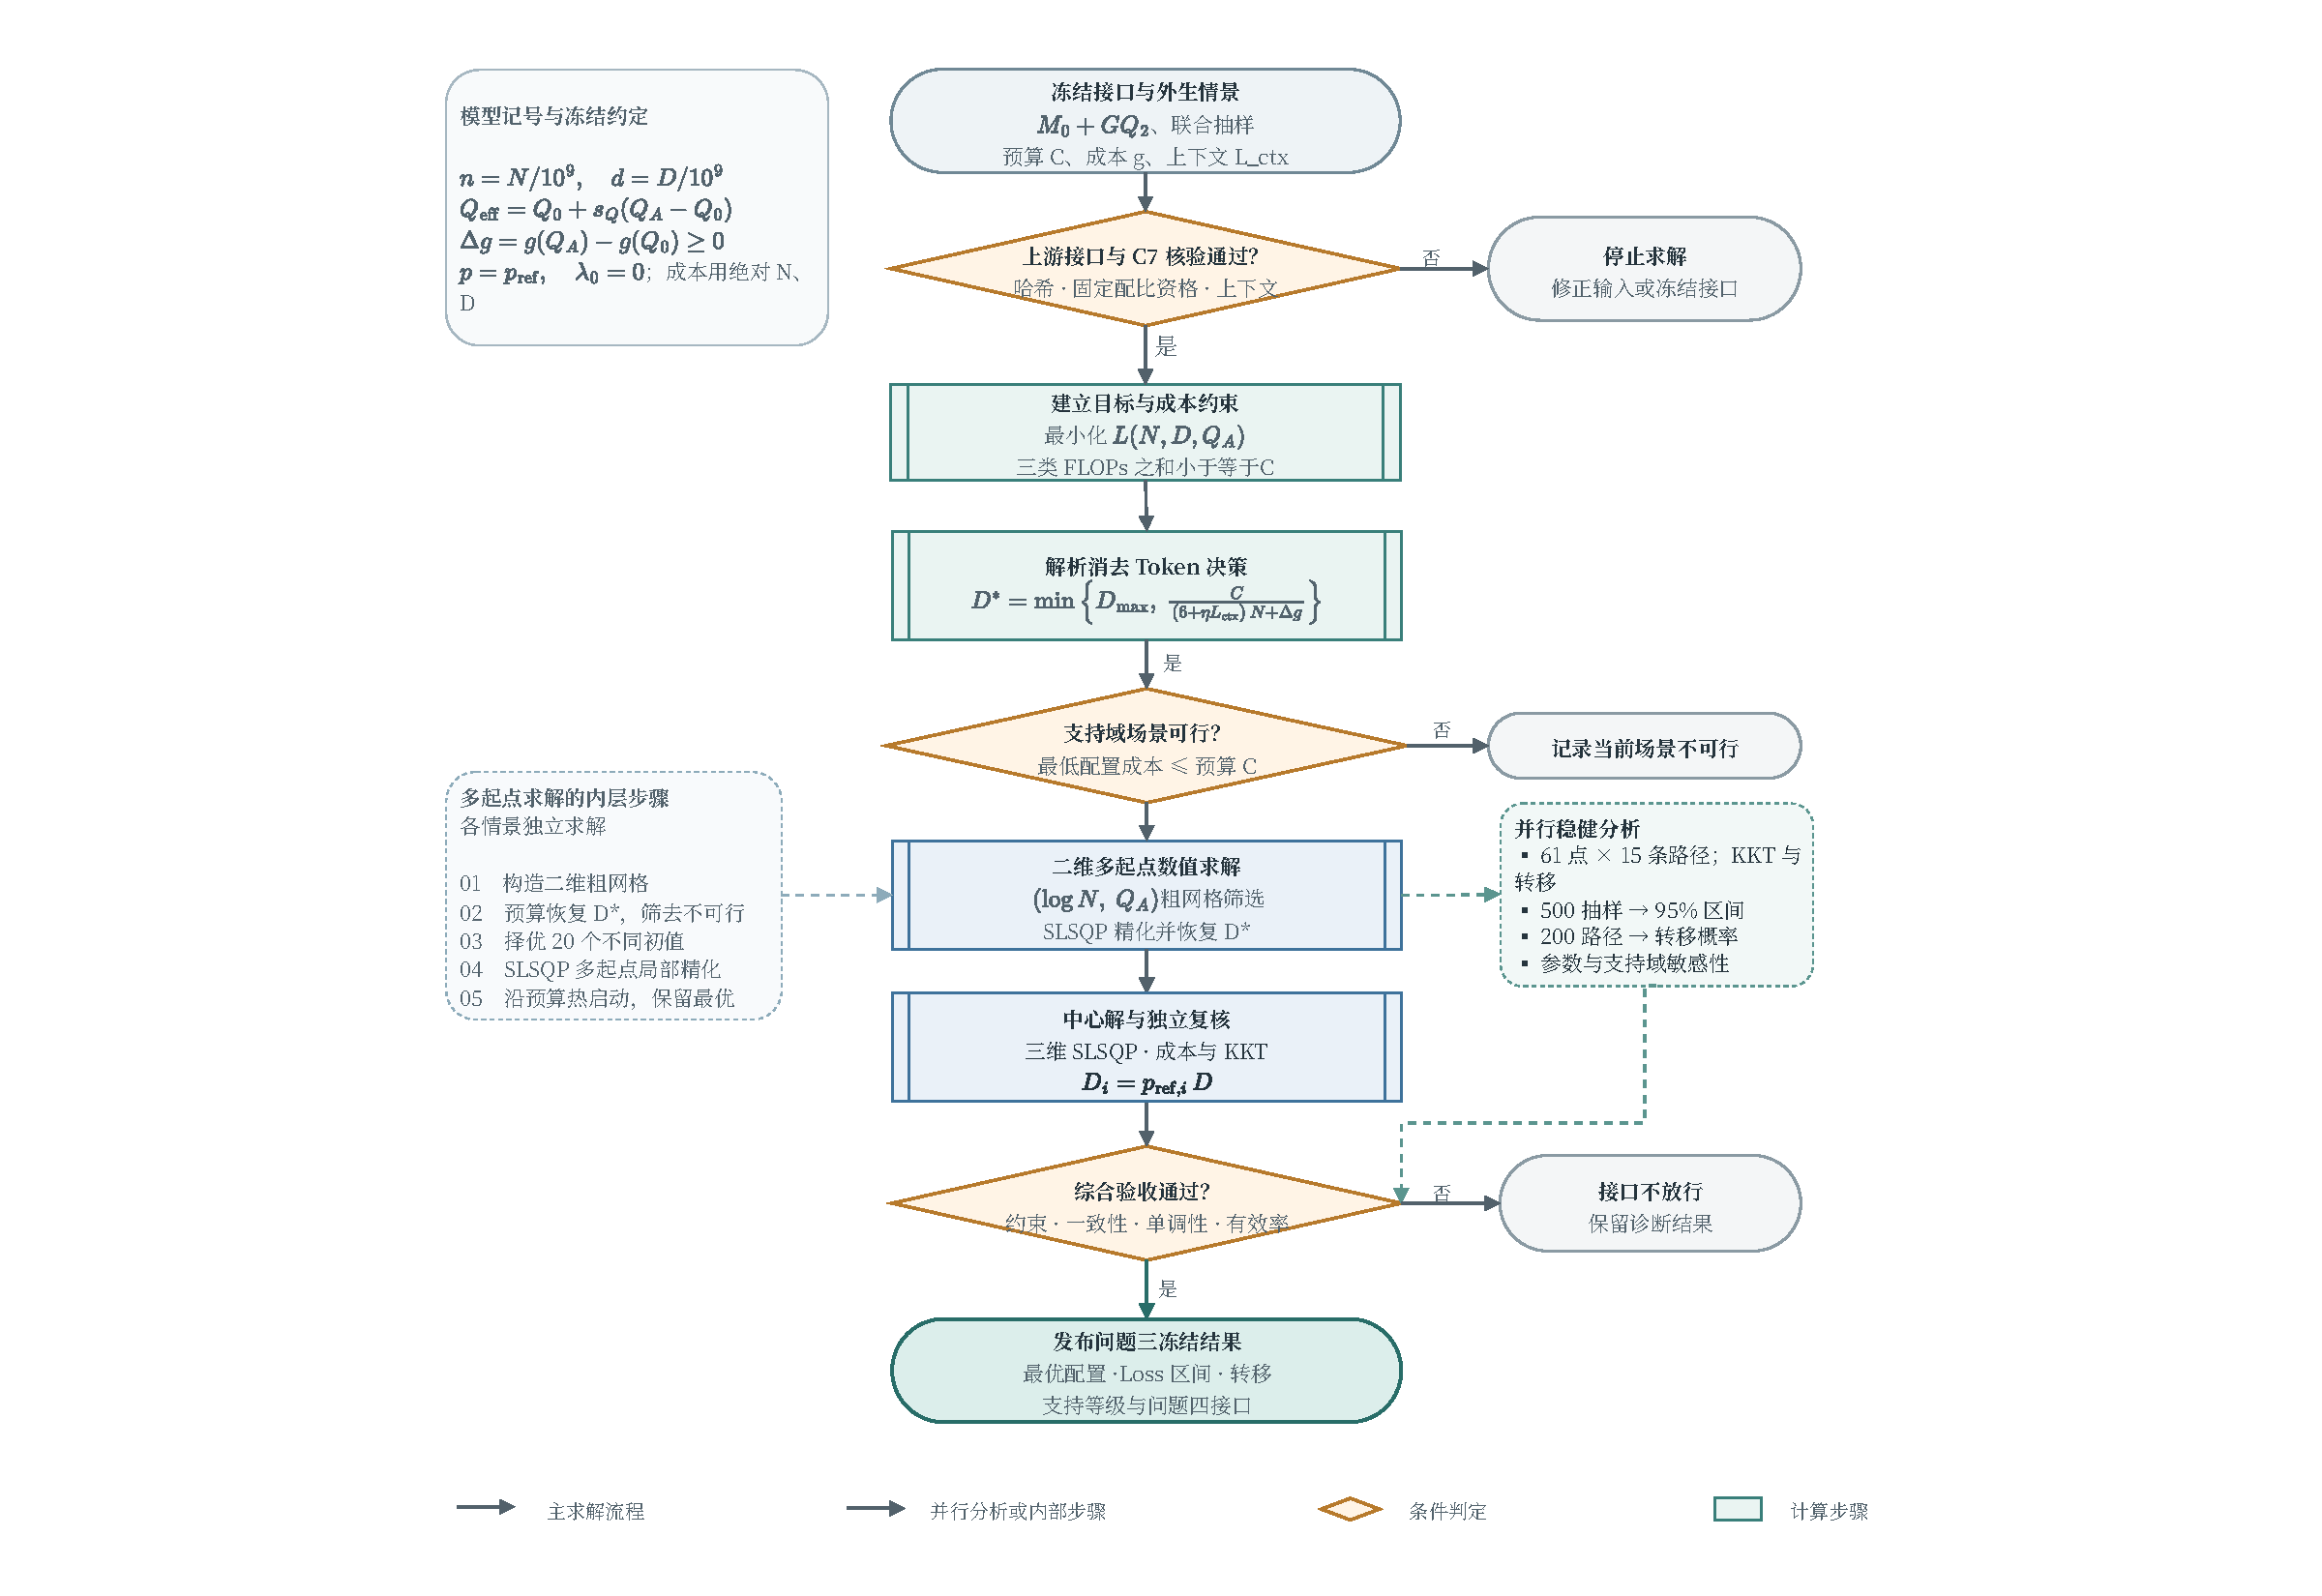
\includegraphics[width=0.78\linewidth,trim=0 90bp 0 0,clip]{images/no3/P3_F00R_问题三资源配置求解流程图.pdf}
\caption{问题三资源配置优化的求解、复核与验收流程}
\label{fig:p3_solver_flow}
\end{figure}

\subsection{资源配置模型的建立}

\subsubsection{冻结输入与决策边界}

本问沿用问题二的参数--数据可分标度律与加性质量惩罚模型，不重复拟合附件 A、B；其基础训练轨迹来自 Pythia 模型族\cite{biderman2023pythia}。将冻结预测 $\widehat L_{\mathrm{main}}$ 简记为

\begin{equation}
L(N,D,Q_A)
=E+A\left(\frac{N}{10^9}\right)^{-\alpha}
+B\left(\frac{D}{10^9}\right)^{-\beta}
+c_Q(1-Q_{\mathrm{eff}})^{\nu_Q},
\label{eq:p3_generalized_scaling}
\end{equation}

其中 $Q_{\mathrm{eff}}$ 为进入损失函数的有效质量。两问的质量变量来自不同实验体系，故以公共参考质量 $Q_0$ 为锚点，作线性对齐并限制其不超过有效上界：

\begin{equation}
\begin{aligned}
Q_{\mathrm{eff}}&=Q_0+s_Q(Q_A-Q_0),
\qquad Q_0=0.5389559588,\\
Q_{\mathrm{sat}}&=\min\left\{1,
Q_0+\frac{1-\varepsilon-Q_0}{s_Q}\right\},
\qquad \varepsilon=10^{-6}.
\end{aligned}
\label{eq:p3_quality_mapping}
\end{equation}

主情景取 $s_Q=1$，并以 $0.5$ 和 $1.5$ 检验跨体系映射敏感性。式~\eqref{eq:p3_generalized_scaling} 的参数沿用问题二中心估计；在合法区间内，增大 $N$、$D$ 或 $Q_A$ 均不会使预测损失上升。表~\ref{tab:p3_interface} 汇总优化接口，避免冻结量、决策量与情景量混用。

\begin{table}[!htbp]
\centering
\small
\setlength{\tabcolsep}{5pt}
\caption{问题三的冻结输入、决策变量与情景变量}
\label{tab:p3_interface}
\begin{tabular}{p{0.18\linewidth}p{0.30\linewidth}p{0.42\linewidth}}
\toprule
类型 & 变量 & 来源或作用 \\
\midrule
冻结输入 & $\boldsymbol p_{\mathrm{ref}},Q_0,E,A,B,\alpha,\beta,c_Q,\nu_Q$ & 由问题一和问题二传入，优化中不重估 \\
决策变量 & $N,D,Q_A$ & 在给定算力预算下最小化冻结 Loss \\
情景变量 & $C,L_{\mathrm{ctx}},g,s_Q$ & 描述预算、上下文、质量成本与映射假设 \\
派生输出 & $D_i=p_{\mathrm{ref},i}D^*$ & 将最优总 Token 数分解到 $17$ 个领域 \\
\bottomrule
\end{tabular}
\end{table}

\subsubsection{三类算力成本与优化约束}

基础训练、质量提升和长文本注意力三类成本分别定义为

\begin{equation}
\begin{aligned}
C_{\mathrm{train}}&=6ND,\\
C_Q&=D\,[g(Q_A)-g(Q_0)]_+,\\
C_{\mathrm{attn}}&=\eta NDL_{\mathrm{ctx}},
\qquad \eta=2\times10^{-4},
\end{aligned}
\label{eq:p3_three_costs}
\end{equation}

其中 $[x]_+=\max(x,0)$，$6ND$ 为常用训练算力近似\cite{kaplan2020scaling,hoffmann2022compute}。自注意力对序列长度具有二次复杂度\cite{vaswani2017attention}；固定总 Token 数后，每个 Token 的附加开销近似正比于上下文长度，故用 $\eta NDL_{\mathrm{ctx}}$ 表示。系数 $\eta$ 为题设情景参数。三种质量成本取

\begin{equation}
\begin{aligned}
g_{\exp}(Q)&=10^7e^{6Q},\\
g_{\mathrm{pow}}(Q)&=5\times10^9Q^4,\\
g_{\log}(Q)&=2\times10^9\ln(1+10Q).
\end{aligned}
\label{eq:p3_quality_costs}
\end{equation}

三种形式表示不同的质量处理成本情景，并非重新拟合的候选模型，故只作并列条件比较。综合上述定义，优化模型为

\begin{equation}
\begin{aligned}
\min_{N,D,Q_A}\quad
&L(N,D,Q_A),\\
\text{s.t.}\quad
&6ND+D[g(Q_A)-g(Q_0)]_+
+\eta NDL_{\mathrm{ctx}}\le C,\\
&N_{\min}\le N\le N_{\max},\\
&D_{\min}\le D\le D_{\max},\\
&Q_0\le Q_A\le Q_{\mathrm{sat}}.
\end{aligned}
\label{eq:p3_optimization}
\end{equation}

成本式中的 $N,D$ 使用绝对数量；式~\eqref{eq:p3_generalized_scaling} 中除以 $10^9$ 仅用于无量纲化，不能把十亿单位直接代入成本式。

\subsubsection{上下文情景与支持域}

附件 C7 的 $45$ 条记录形成 $2048$、$4096$、$8192$、$32768$ 和 $131072$ 五档上下文。鉴于部分架构字段不一致，本问只使用独立核验后的上下文窗口，并将五档视为等权外生情景。为区分观测支持内结论与外推结果，设置

\begin{equation}
\begin{array}{lll}
\text{严格共同支持域：}&N\in[0.070542,11.965825]\ \mathrm{B},
&D\in[10,299.893]\ \mathrm{B},\\
\text{条件扩展域：}&N\in[0.070542,10000]\ \mathrm{B},
&D\in[0.1,36000]\ \mathrm{B}.
\end{array}
\label{eq:p3_support_domains}
\end{equation}

严格域用于检验参数项和质量项均有数据覆盖的结果，扩展域用于回答三档预算。每个解标记为共同观测支持、单分量外推、桥接缺口外推或边界支持外推；严格域不可行时如实报告，超出扩展域的方案判为无效。

\subsection{模型求解}

\subsubsection{解析降维与多起点优化}

将总成本写成

\begin{equation}
C_{\mathrm{tot}}
=D\left[(6+\eta L_{\mathrm{ctx}})N
+\Delta g(Q_A)\right],
\qquad
\Delta g(Q_A)=[g(Q_A)-g(Q_0)]_+.
\label{eq:p3_cost_rearranged}
\end{equation}

由式~\eqref{eq:p3_generalized_scaling} 可知，固定 $(N,Q_A)$ 时有 $\partial L/\partial D<0$，因此应把剩余预算全部用于增加训练 Token 数。预算允许的最大数据量为

\begin{equation}
D^{\max}(N,Q_A)
=\frac{C}{(6+\eta L_{\mathrm{ctx}})N+\Delta g(Q_A)},
\label{eq:p3_dmax}
\end{equation}

考虑搜索上界后取

\begin{equation}
D^*(N,Q_A)
=\min\{D_{\max},D^{\max}(N,Q_A)\},
\qquad D^*(N,Q_A)\ge D_{\min}.
\label{eq:p3_dstar}
\end{equation}

三维约束优化由此降为 $(\log N,Q_A)$ 上的二维有界优化。每个成本函数、上下文、预算、质量映射和支持域组合均先进行粗网格搜索，再从目标值最小的二十个不同网格点出发作局部精化；沿预算递增方向，以上一预算的最优解作为连续追踪初值。三档预算、三种成本和五档上下文构成的 $45$ 个中心情景，另用完整三维非线性规划独立求解，并以加密网格检查局部最优风险。

图~\ref{fig:p3_low_budget_landscape} 以 $4096$ 上下文和 $10^{19}$ FLOPs 为例展示降维后的目标景观。三个谷底均体现参数量与质量的替代关系，但不同质量成本改变了谷底沿 $Q_A$ 方向的位置：指数成本形成内点解，幂函数成本停留在质量基线，对数成本则到达质量上界。这也说明多起点搜索和边界识别不可省略。

\begin{figure}[!htbp]
\centering
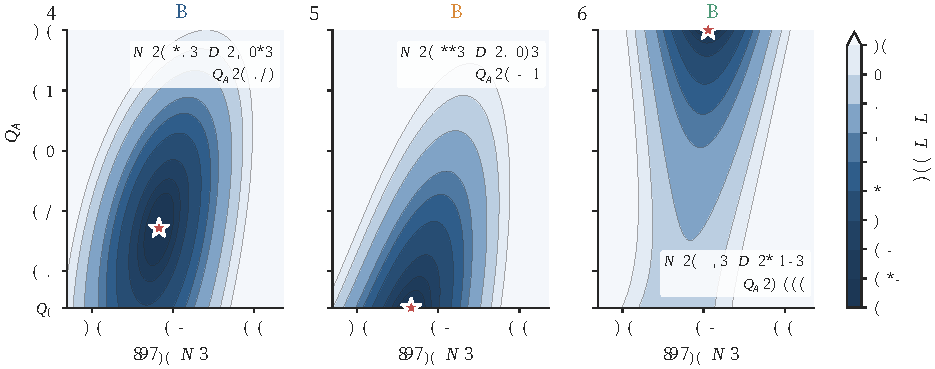
\includegraphics[width=0.94\linewidth]{images/no3/P3_F03_三类质量成本下的低预算优化景观.pdf}
\caption{$4096$ 上下文、$10^{19}$ FLOPs 下三类质量成本的解析降维景观}
\label{fig:p3_low_budget_landscape}
\end{figure}

在实现层面，算法~\ref{alg:p3_solver} 给出二维求解、三维复核、预算连续追踪和结构转移筛选的可复现顺序。

\begin{algorithm}[!htbp]
\caption{算力约束下资源配置与结构转移识别}
\label{alg:p3_solver}
\begin{algorithmic}[1]
\Require 冻结参数 $\boldsymbol\theta$、参考配比 $\boldsymbol p_{\mathrm{ref}}$、预算 $\mathcal C$、上下文 $\mathcal L$、成本集合 $\mathcal G$、支持域 $\mathcal S$
\Ensure 中心最优解、领域 Token 配置、活跃约束与稳定转移点
\ForAll{$g\in\mathcal G$，$L_{\mathrm{ctx}}\in\mathcal L$，$\mathcal S$}
    \ForAll{按升序排列的 $C\in\mathcal C$}
        \State 由式~\eqref{eq:p3_dstar} 计算粗网格，并删除不可行点
        \State 取最优的 $20$ 个网格点和上一预算解作为初值
        \State 对各初值执行二维有界局部精化，取 Loss 最小的可行解 $\boldsymbol x^*(C)$
        \If{$C\in\{10^{19},10^{22},10^{24}\}$}
            \State 使用完整三维非线性规划与加密网格独立复核 $\boldsymbol x^*(C)$
        \EndIf
        \State 记录成本份额、支持状态及 $D_i=p_{\mathrm{ref},i}D^*$
    \EndFor
\State 比较相邻预算的活跃集合，并用配置弹性与 BIC 筛选次要断点
\EndFor
\State 以 $500$ 次锚点 bootstrap 和 $200$ 条联合抽样路径传播不确定性
\State 输出出现概率不低于 $70\%$ 的结构转移
\end{algorithmic}
\end{algorithm}

当 $Q_A=Q_0$ 且变量边界均未激活时，令 $n=N/10^9$、$d=D/10^9$、$\overline C=C/[(6+\eta L_{\mathrm{ctx}})10^{18}]$，不含质量投资的部分具有闭式基准

\begin{equation}
n^*
=\left(\frac{\alpha A}{\beta B}\right)^{1/(\alpha+\beta)}
\overline C^{\beta/(\alpha+\beta)},
\qquad
d^*=\frac{\overline C}{n^*}.
\label{eq:p3_classic_closed_form}
\end{equation}

该结果仅用于初始化和公式回归，不替代正式优化结果。

\subsubsection{KKT边际解释}

在满足约束资格条件、预算约束活跃且三类决策均位于内点时，KKT 必要条件要求三种资源的单位算力边际收益相等\cite{nocedal2006numerical}：

\begin{equation}
\frac{-L_N}{C_N}
=\frac{-L_D}{C_D}
=\frac{-L_Q}{C'_Q},
\label{eq:p3_kkt_ratio}
\end{equation}

其中

\begin{equation}
\begin{aligned}
C_N&=(6+\eta L_{\mathrm{ctx}})D,\\
C_D&=(6+\eta L_{\mathrm{ctx}})N+\Delta g(Q_A),\\
C'_Q&=Dg'(Q_A).
\end{aligned}
\label{eq:p3_marginal_costs}
\end{equation}

式~\eqref{eq:p3_kkt_ratio} 给出了资源配置的直接解释：若质量下界乘子为正，则当前预算下新增算力投入质量不如投入参数或 Token；当该乘子降为零并且 $Q_A$ 离开 $Q_0$ 时，质量投资才被启用；当 $Q_A$ 达到 $Q_{\mathrm{sat}}$ 后，新增预算重新主要流向参数和数据扩张。

\subsubsection{结构性转移的数学定义}

固定质量成本、上下文、质量尺度和支持域，定义预算 $C$ 下最优解的活跃集合

\begin{equation}
\mathcal A(C)=
\{Q_A=Q_0,\ Q_A=Q_{\mathrm{sat}},\
N=N_{\min/\max},\ D=D_{\min/\max},\
C_{\mathrm{tot}}=C\}.
\label{eq:p3_active_set}
\end{equation}

若临界预算两侧满足 $\mathcal A(C^-)\neq\mathcal A(C^+)$，则记为主要转移；对活跃集合不变的区段，再计算配置弹性

\begin{equation}
\theta_x(C)=\frac{\mathrm d\log x^*}{\mathrm d\log C},
\qquad x\in\{N,D,Q_A-Q_0\}.
\label{eq:p3_configuration_elasticity}
\end{equation}

分段线性拟合相对单直线的 BIC 改善不低于 $10$ 且断点两侧斜率差不低于 $0.15$ 时，记为次要候选\cite{schwarz1978estimating}。转移点由 $61$ 个对数预算点夹逼，主要转移再二分至 $\log_{10}C$ 区间宽度不超过 $0.01$；同类事件在至少 $70\%$ 的抽样路径中出现时，才称为稳定转移。

\subsection{结果分析与模型验证}

\subsubsection{上下文临界长度}

由式~\eqref{eq:p3_three_costs} 可知，注意力成本和基础训练成本之比为

\begin{equation}
\frac{C_{\mathrm{attn}}}{C_{\mathrm{train}}}
=\frac{\eta L_{\mathrm{ctx}}}{6}.
\label{eq:p3_attention_ratio}
\end{equation}

令该比值等于 $1$，得到两类成本相等的临界上下文长度

\begin{equation}
L_{\mathrm{ctx}}^{\mathrm{crit}}
=\frac{6}{\eta}=30000.
\label{eq:p3_context_critical}
\end{equation}

五档上下文对应的上述比值依次为 $0.0683$、$0.1365$、$0.2731$、$1.0923$ 和 $4.3691$，故后两档已经越过临界点。图~\ref{fig:p3_context_penalty} 进一步以 $2048$ Token 为基准，比较上下文增长带来的最优 Loss 增量。

\begin{figure}[!htbp]
\centering
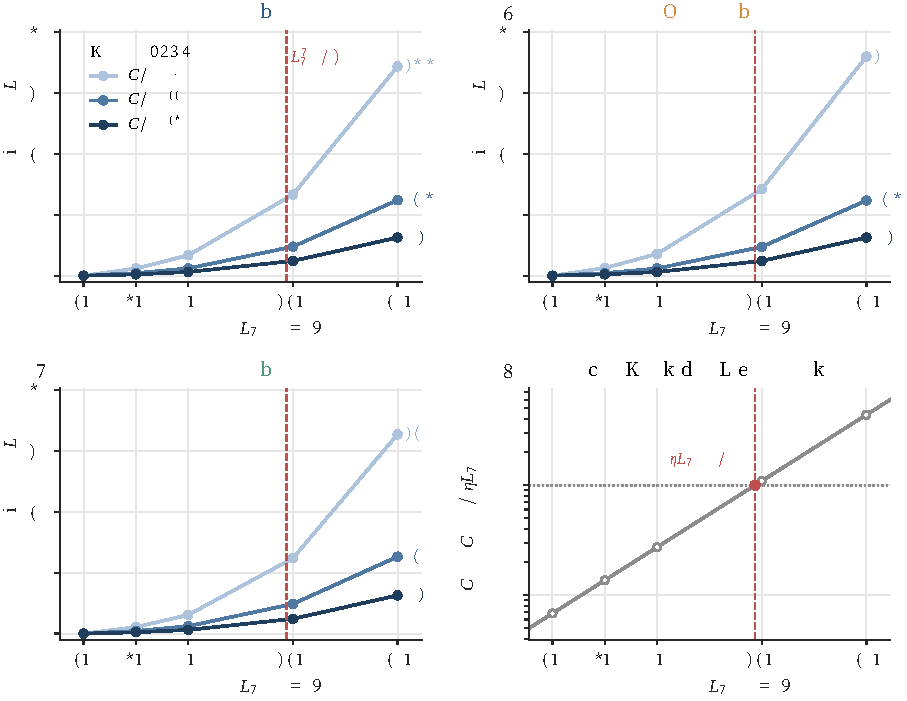
\includegraphics[width=0.94\linewidth]{images/no3/P3_F02_上下文成本临界与最优损失惩罚.pdf}
\caption{上下文长度引起的最优 Loss 增量与 $30000$ Token 临界线}
\label{fig:p3_context_penalty}
\end{figure}

跨过 $30000$ Token 后，三类成本情景的惩罚均明显扩大；在 $131072$ Token 下，$10^{19}$ FLOPs 的 $100\Delta L$ 达 $32.7$--$36.0$，而 $10^{24}$ FLOPs 约为 $6.3$。长上下文会挤压低预算下本已有限的参数和数据投入，高预算则能通过扩大规模部分吸收影响。需注意，式~\eqref{eq:p3_attention_ratio} 与预算及最优解无关，因此 $30000$ 描述上下文成本临界，而非随预算增加产生的结构转移。

最优 Loss 的变化来自最优配置的内生调整。图~\ref{fig:p3_context_response} 将 $N^*$ 和 $D^*$ 分别对 $2048$ Token 情景归一化，并同时给出质量决策 $Q_A^*$。

\begin{figure}[!htbp]
\centering
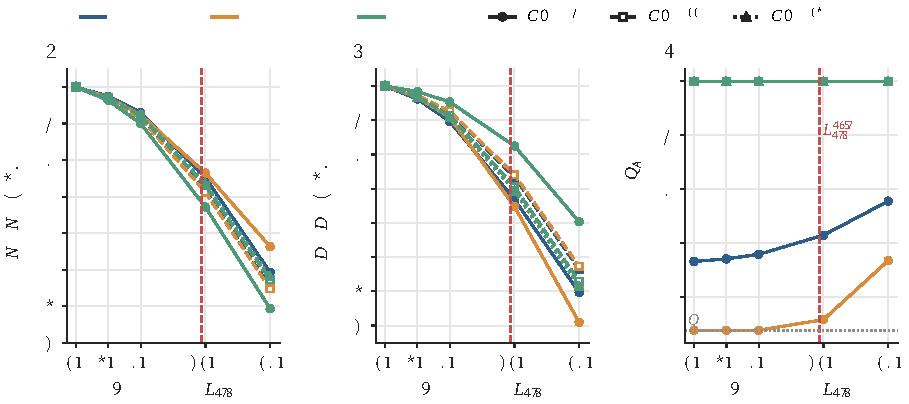
\includegraphics[width=0.94\linewidth]{images/no3/P3_F04_上下文长度对最优配置的影响.pdf}
\caption{上下文长度对三类质量成本最优配置的影响}
\label{fig:p3_context_response}
\end{figure}

参数量和 Token 量均随上下文增长而下降，且数据量通常压缩更快。以低预算指数成本为例，$131072$ Token 时 $N^*$、$D^*$ 分别降至基准的 $49.3\%$、$39.7\%$，而 $Q_A^*$ 由 $0.666$ 升至 $0.778$。未饱和时，提高质量可部分对冲规模收缩；质量饱和后，长上下文成本只能由 $N^*$ 与 $D^*$ 共同吸收。

\subsubsection{三档预算下的最优资源配置}

以 $L_{\mathrm{ctx}}=4096$、$s_Q=1$ 和条件扩展域为主展示情景，三档预算下的中心最优配置见表~\ref{tab:p3_anchor_allocations}。表中 $N$ 和 $D$ 均以十亿为单位；为突出问题三的资源配置结论，仅保留最优决策、预测 Loss 和支持状态，三类成本份额在正文中解释。

\begin{table}[!htbp]
\centering
\caption{4096上下文下三档预算的中心最优配置}
\label{tab:p3_anchor_allocations}
\footnotesize
\setlength{\tabcolsep}{3.5pt}
\begin{tabular}{llrrrrl}
\toprule
质量成本 & 预算/FLOPs & $N^*$ & $D^*$ & $Q_A^*$ & $L^*$ & 支持状态 \\
\midrule
指数 & $10^{19}$ & $0.259187$ & $4.82101$ & $0.671056$ & $3.16898$ & 单分量外推 \\
指数 & $10^{22}$ & $5.44886$ & $244.275$ & $0.999999$ & $2.15491$ & 共同观测支持 \\
指数 & $10^{24}$ & $39.5804$ & $3653.81$ & $0.999999$ & $1.91601$ & 桥接缺口外推 \\
\midrule
幂函数 & $10^{19}$ & $0.215205$ & $6.81420$ & $0.538956$ & $3.17962$ & 单分量外推 \\
幂函数 & $10^{22}$ & $5.55840$ & $235.394$ & $0.999999$ & $2.15634$ & 共同观测支持 \\
幂函数 & $10^{24}$ & $39.7119$ & $3631.33$ & $0.999999$ & $1.91611$ & 桥接缺口外推 \\
\midrule
对数 & $10^{19}$ & $0.337313$ & $2.95276$ & $0.999999$ & $3.11805$ & 单分量外推 \\
对数 & $10^{22}$ & $5.04774$ & $281.627$ & $0.999999$ & $2.14976$ & 共同观测支持 \\
对数 & $10^{24}$ & $39.1302$ & $3732.41$ & $0.999999$ & $1.91566$ & 桥接缺口外推 \\
\bottomrule
\end{tabular}
\end{table}

低预算下三类路径差异最大，与图~\ref{fig:p3_low_budget_landscape} 的谷底位置一致：指数成本选择内点质量 $Q_A=0.671056$，幂函数成本停留在 $Q_0$，对数成本达到质量上界并以 $32.08\%$ 的预算提质。其 Loss 最低只表示该题设成本下的条件结果，不能反推真实质量处理必然服从对数成本。三种低预算解均属单分量外推，主要用于比较机制。

预算提高到 $10^{22}$ FLOPs 后，三类成本均达到质量上界且处于共同观测支持域；到 $10^{24}$ FLOPs，最优参数量约为 $39.1$--$39.7$ B、数据量约为 $3.63$--$3.73$ 万亿 Token，三类 Loss 差异小于 $5\times10^{-4}$。这表明质量饱和后，新增预算重新流向参数和数据扩张，成本函数形状的影响迅速减弱。

每个方案再按式~\eqref{eq:p3_fixed_mixture} 分解为十七个领域的 Token 数，满足 $D_i\ge0$ 和 $\sum_iD_i=D$，从而把最优总数据量转化为可执行的领域预算。

\subsubsection{连续预算路径与成本份额}

在 $4096$ 上下文的连续预算路径上，$N^*$ 和 $D^*$ 总体近似幂律增长，而质量路径呈阶段差异：对数成本从起点即饱和，指数成本从中等质量继续上升，幂函数成本则先保持基线再启动提质。

\begin{figure}[!htbp]
\centering
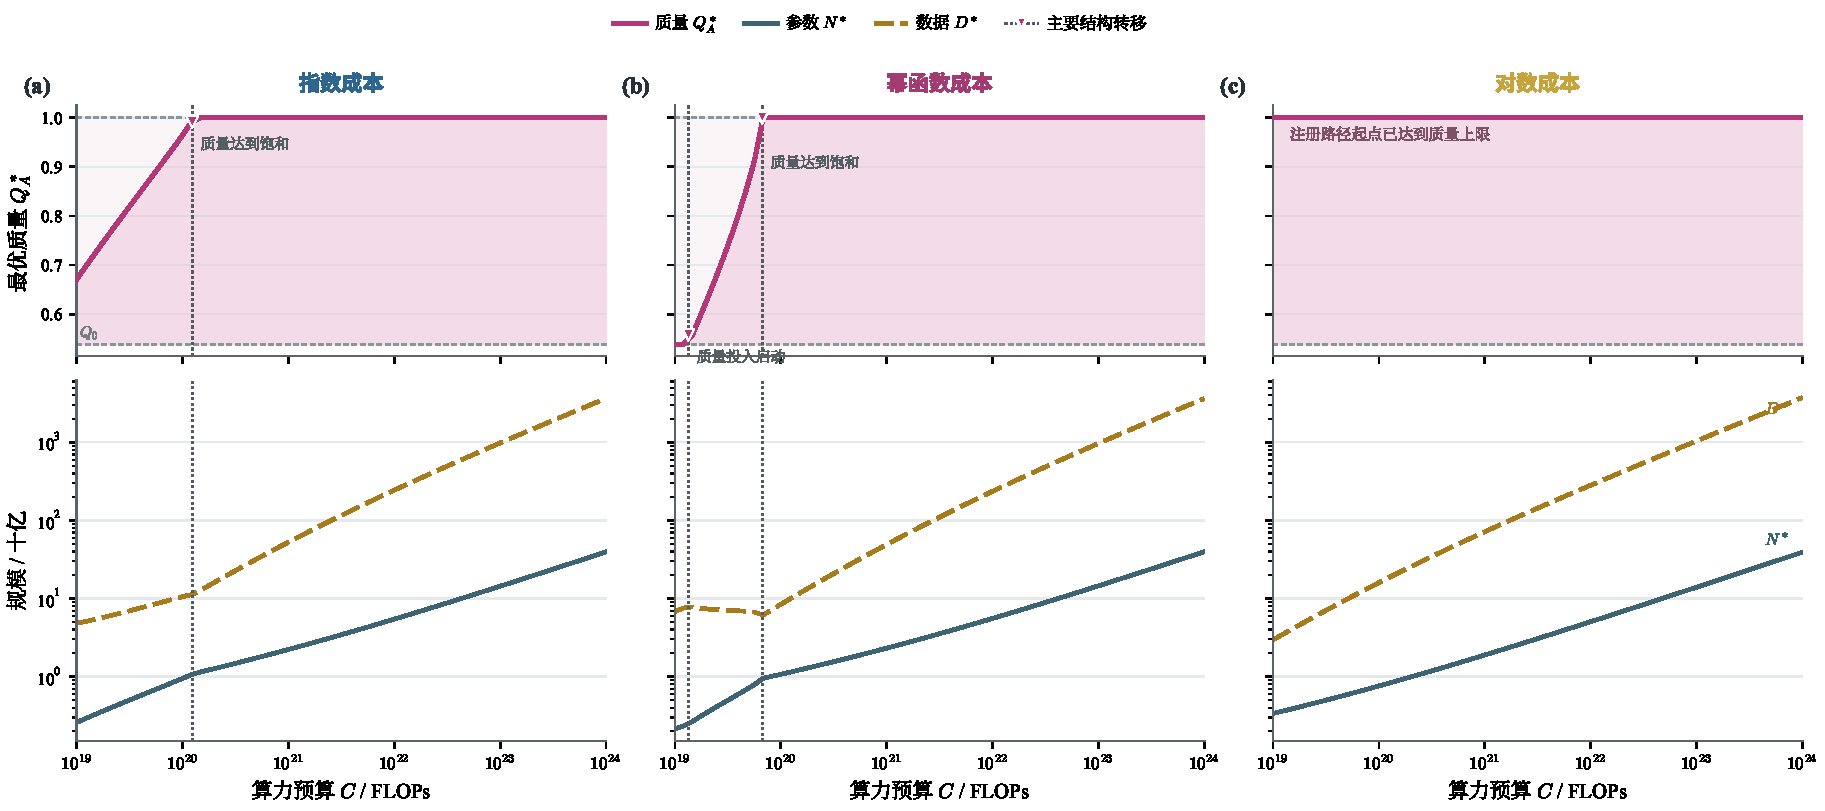
\includegraphics[width=0.94\linewidth]{images/no3/P3_F07_最优配置路径与结构转移.pdf}
\caption{$4096$ 上下文下的连续最优配置路径与结构转移}
\label{fig:p3_configuration_paths}
\end{figure}

图~\ref{fig:p3_configuration_paths} 将质量状态与参数--Token 扩张对齐。幂函数路径在 $1.342\times10^{19}$ FLOPs 离开 $Q_0$、在 $6.691\times10^{19}$ FLOPs 饱和；指数路径在 $1.234\times10^{20}$ FLOPs 饱和。质量曲线变平后 $N^*$ 与 $D^*$ 仍增长，说明新增预算已转回规模扩张。

固定上下文时，注意力与基础训练成本的相对比例不变，因此份额变化主要来自质量成本与规模成本的竞争。指数和幂函数情景的质量份额先升后降，对数情景则从高位单调下降；高预算区间均由基础训练成本主导。

\begin{figure}[!htbp]
\centering
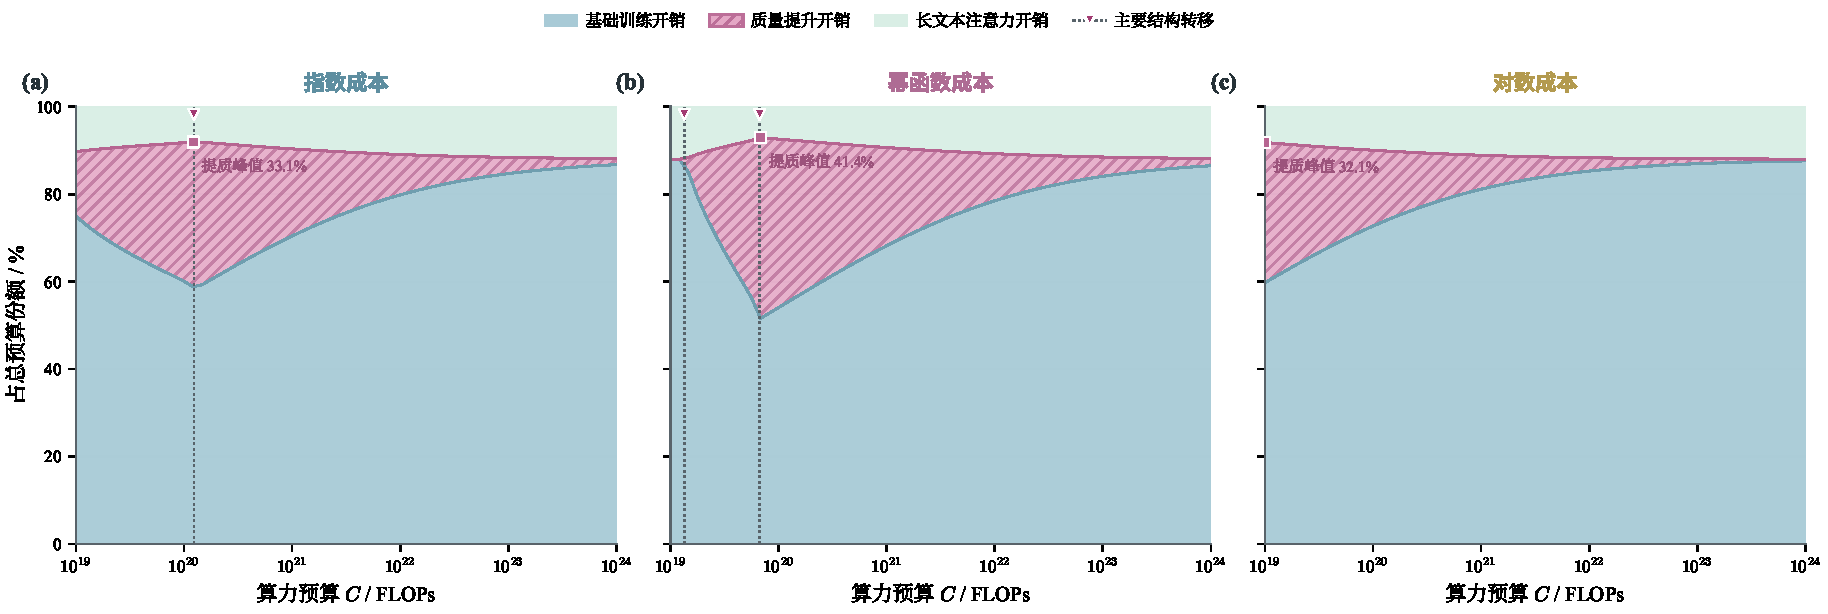
\includegraphics[width=0.94\linewidth]{images/no3/P3_F01_预算约束下的边际资源竞争机制.pdf}
\caption{$4096$ 上下文下连续预算路径的算力份额分解}
\label{fig:p3_budget_shares}
\end{figure}

图~\ref{fig:p3_budget_shares} 中三类质量份额峰值分别约为 $33.1\%$、$41.4\%$ 和 $32.1\%$。质量带的扩张与收缩直接对应式~\eqref{eq:p3_kkt_ratio} 的边际竞争；达到上限后，其份额被持续增长的规模成本稀释。

\subsubsection{稳定结构性转移}

$4096$ 上下文下通过稳定性门槛的转移见表~\ref{tab:p3_transitions}。指数成本依次出现质量弹性断点、质量饱和和数据量弹性断点；幂函数成本则完整经历“保持基线--启动提质--质量饱和--规模扩张”，具体临界预算由表中给出。

\begin{table}[!htbp]
\centering
\caption{4096上下文下的稳定结构性转移}
\label{tab:p3_transitions}
\small
\setlength{\tabcolsep}{5pt}
\begin{tabular}{lllrr}
\toprule
质量成本 & 层级 & 转移事件 & 临界预算/FLOPs & 出现概率 \\
\midrule
指数 & 次要 & 质量增量弹性断点 & $9.085\times10^{19}$ & $1.000$ \\
指数 & 主要 & 质量达到饱和 & $1.234\times10^{20}$ & $1.000$ \\
指数 & 次要 & 数据量弹性断点 & $2.371\times10^{20}$ & $1.000$ \\
\midrule
幂函数 & 主要 & 质量投资启动 & $1.342\times10^{19}$ & $1.000$ \\
幂函数 & 次要 & 质量增量弹性断点 & $4.217\times10^{19}$ & $1.000$ \\
幂函数 & 主要 & 质量达到饱和 & $6.691\times10^{19}$ & $1.000$ \\
幂函数 & 次要 & 参数量弹性断点 & $1.101\times10^{20}$ & $1.000$ \\
幂函数 & 次要 & 数据量弹性断点 & $1.101\times10^{20}$ & $1.000$ \\
\bottomrule
\end{tabular}
\end{table}

中心参数下的单一临界值不足以衡量事件定位的可靠性。图~\ref{fig:p3_transition_bootstrap} 因此同时给出两个关键转移事件在 $200$ 条联合参数路径上的二维分布及边缘分布。

\begin{figure}[!htbp]
\centering
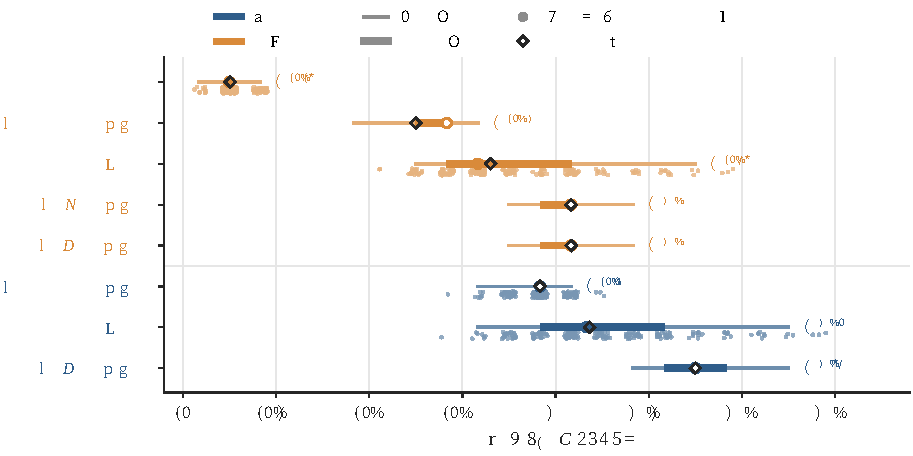
\includegraphics[width=0.92\linewidth]{images/no3/P3_F05_稳定结构转移的区间估计.pdf}
\caption{$4096$ 上下文下关键结构转移预算的联合 bootstrap 分布}
\label{fig:p3_transition_bootstrap}
\end{figure}

指数成本下，质量弹性断点与饱和位置呈较强正相关（$\rho=0.81$）；幂函数成本下启动与饱和位置的相关系数仅为 $-0.08$。中心结果均位于 bootstrap 主体区域，事件出现概率均为 $1$。主要、次要转移的 $\log_{10}C$ 定位区间宽度分别为 $0.00521$、$0.08333$。对数成本在路径起点已达质量上界，故当前预算范围内没有新的质量状态转移。

因此，资源配置可概括为三个阶段：低预算下保持质量基线，跨过阈值后质量与规模竞争，质量饱和后新增算力重新集中到参数和数据扩张。阶段边界随成本函数和上下文变化，但该机制在可行情景中一致。

\subsection{敏感性、适用边界与本问输出}

\subsubsection{参数不确定性传播}

每个中心情景以 $500$ 组联合参数 bootstrap 样本传播问题二参数和参考质量的不确定性\cite{efron1979bootstrap}。表~\ref{tab:p3_bootstrap_loss} 表明，低预算下质量参数影响较明显，幂函数成本区间最宽；质量饱和后各区间均显著收窄。

\begin{table}[!htbp]
\centering
\caption{4096上下文下最优Loss的bootstrap区间}
\label{tab:p3_bootstrap_loss}
\small
\setlength{\tabcolsep}{6pt}
\begin{tabular}{llrrr}
\toprule
质量成本 & 预算/FLOPs & 中位数 & $2.5\%$分位数 & $97.5\%$分位数 \\
\midrule
指数 & $10^{19}$ & $3.16903$ & $3.15657$ & $3.18222$ \\
指数 & $10^{22}$ & $2.15491$ & $2.15488$ & $2.15493$ \\
指数 & $10^{24}$ & $1.91601$ & $1.91595$ & $1.91607$ \\
\midrule
幂函数 & $10^{19}$ & $3.18002$ & $3.16432$ & $3.19592$ \\
幂函数 & $10^{22}$ & $2.15634$ & $2.15631$ & $2.15636$ \\
幂函数 & $10^{24}$ & $1.91611$ & $1.91605$ & $1.91617$ \\
\midrule
对数 & $10^{19}$ & $3.11805$ & $3.11728$ & $3.11871$ \\
对数 & $10^{22}$ & $2.14975$ & $2.14972$ & $2.14978$ \\
对数 & $10^{24}$ & $1.91567$ & $1.91560$ & $1.91572$ \\
\bottomrule
\end{tabular}
\end{table}

连续预算路径另分层选取 $200$ 组联合样本估计转移概率，以保留 $E,A,B,\alpha,\beta,c_Q,\nu_Q$ 与 $Q_0$ 之间的相关结构。

\subsubsection{敏感性与证据边界}

敏感性分析包含 $234$ 个场景，覆盖质量映射斜率、质量成本与注意力系数的 $\pm20\%$ 扰动、经验质量上界及严格共同支持域。质量映射主要影响低预算下是否启动提质；质量饱和后，Loss 对该斜率的敏感性明显降低。

\begin{figure}[!htbp]
\centering
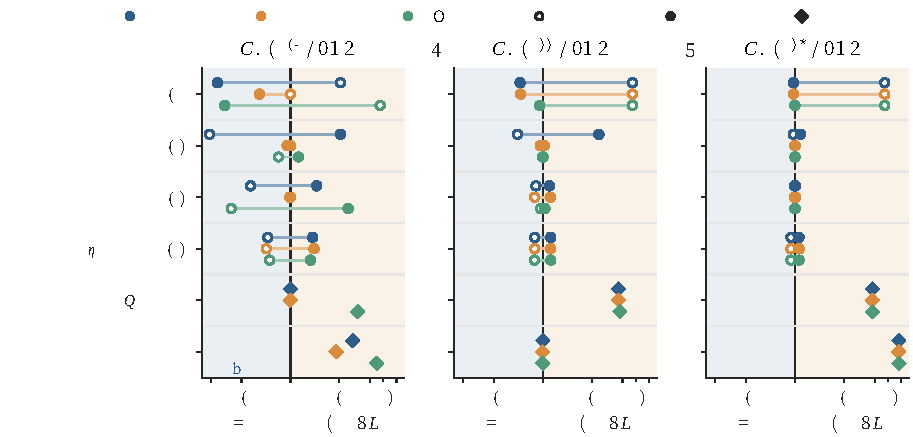
\includegraphics[width=0.92\linewidth]{images/no3/P3_F06_关键假设的敏感性分析.pdf}
\caption{$4096$ 上下文下关键假设对最优 Loss 的敏感性}
\label{fig:p3_sensitivity}
\end{figure}

图~\ref{fig:p3_sensitivity} 中，$10^{19}$ FLOPs 下点位最分散；到 $10^{22}$ 和 $10^{24}$ FLOPs，多数双侧扰动收缩到零附近。严格支持域检查在高预算下仍使 Loss 明显上升，这是扩展域最优规模被观测边界截断所致，而非局部参数不稳定。

$45$ 个中心情景中有 $30$ 个带外推标记：$10^{19}$ FLOPs 主要为单分量外推，$10^{22}$ FLOPs 主展示结果位于共同观测支持域，$10^{24}$ FLOPs 则跨越桥接缺口。因此，高预算结果属于冻结标度律边界内的条件推断，而非新增实测证据。

\subsubsection{数值验收}

本文逐项回代成本、边界、单位、预算、二维--三维一致性、加密网格与领域 Token 守恒。Loss 重建误差和同种子重复相对差均为 $0$；约束违反量、二维--三维 Loss 相对差、加密网格相对差和 Token 求和误差分别为 $4.096\times10^{-16}$、$4.381\times10^{-14}$、$2.063\times10^{-16}$ 和 $1.860\times10^{-16}$，均通过门槛。

多起点优化的过程性证据见图~\ref{fig:p3_multistart}。该图选取低预算指数成本情景，因为此时质量位于内点，比质量已饱和的情景更能检验二维谷地中的局部最优风险。

\begin{figure}[!htbp]
\centering
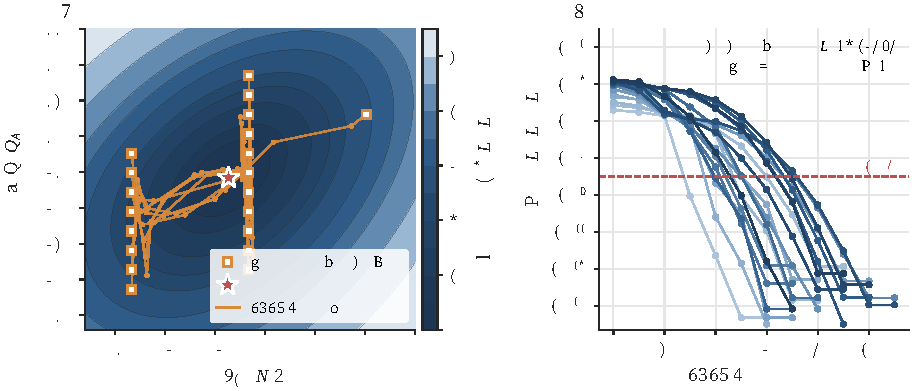
\includegraphics[width=0.88\linewidth]{images/no3/P3_F08_多起点寻优过程与收敛验证.pdf}
\caption{指数成本低预算情景的多起点寻优轨迹与局部收敛验证}
\label{fig:p3_multistart}
\end{figure}

二十个候选起点全部收敛，三条代表性路径从不同位置汇聚到表~\ref{tab:p3_anchor_allocations} 中的指数成本低预算解，相对 Loss 差距降至数值零附近。结合加密网格和完整三维复核，可排除单一初值造成的局部最优假象。全部中心解还满足成本非负、预算可行、最优值随预算不增加以及长上下文不降低 Loss 等物理门禁。

综上，模型把参数、训练 Token、质量和长上下文成本统一到预算框架，识别出“未启动提质--质量参与竞争--质量饱和后规模重新主导”的阶段变化。结论受三项边界约束：领域配比绝对强度尚未识别，质量成本为题设情景，高预算含明显外推，故只能解释为给定模型和支持域内的条件最优。

问题四接收 $3$ 种质量成本、$5$ 档上下文和 $3$ 档预算构成的 $45$ 个冻结情景，并携带最优 $(N^*,D^*,Q_A^*)$、Loss 抽样及支持标记。这些结果仅用于 Loss--Benchmark 映射，不重复作为历史能力前沿的训练样本。


\section{问题四模型的建立与求解}
\label{sec:problem4}

\subsection{问题分析与建模思路}

问题四要求把前三问在交叉熵 Loss 尺度上的资源配置结论转换为可比较的下游能力，并进一步回答两个问题：开源大语言模型的历史能力提升有多少与训练规模扩张相关，有多少表现为控制已观测规模后的非规模残余；当训练算力增速放缓时，未来 $12$ 个月和 $24$ 个月的能力前沿将如何变化。已有研究表明，规模扩张与训练算法改进都能推动语言模型性能提升，但预训练 Loss 不能完全解释下游表现，相同 Loss 的模型仍可能具有不同的迁移能力\cite{ho2024algorithmicprogress,liu2023samepretraining}。因此，本文不把 Loss、训练算力与 Benchmark 视为可无误差互换的同一指标，而是建立带有支持域标记和不确定性传播的分层模型。

附件 C 的三类证据在样本规模和可比程度上差异明显。C1/C2 提供统一六任务口径的大样本能力面板，C4 提供较稀疏但可追溯的训练算力和开放权重证据，C6 则提供 Loss 与 Benchmark 的局部配对。若将三类记录直接拼接，既会重复计算同一排行榜记录，也会把桥接预测误当成历史观测。为此，本文依次完成能力量表重建、Loss--Benchmark 单调桥接、动力学能力前沿拟合、贡献分解和算力情景预测；问题三的 $45$ 个冻结方案只在桥接完成后映射为能力情景，不进入历史前沿训练集。

本文采用观察性动力学分解而非严格因果推断。后文所称“规模扩张相关贡献”指模型中训练算力变化对应的预测增量；“非规模残余技术贡献”是控制已观测规模后的时间状态增量，其中仍可能包含数据、架构、优化、后训练及未观测混杂，不能等同于纯算法进步。

\subsection{输入、数据与证据边界}

\subsubsection{数据去重、开放口径与模型分层}

主能力面板优先使用 C2，并以 C1 核验六项得分。原始 $4576$ 条记录经版本级去重后保留 $4546$ 条；主时间轴取提交日期，其有效范围为 2024 年 6 月 8 日至 2025 年 3 月 13 日。开放口径要求 C2 或高置信 C4 匹配明确给出开放权重证据；严格敏感性还要求许可证允许研究和复现，许可证缺失不自动视为 unrestricted。模型类型分为 pretrained、posttrained、merge 和 excluded，确认性贡献分解只使用 pretrained 与 continuously pretrained，以避免将微调收益或基座算力重复归入预训练规模。

C1/C2 与 C4 的实体匹配同时核对规范化名称、组织、模型族、版本和参数量。由此接受 $66$ 条 C4 匹配，最终得到 $41$ 条确认性前沿样本，覆盖 $7$ 个有效月份和 $13$ 个模型家族。posttrained 层仅有 $6$ 条合格算力记录，未达到独立分解所需的支持度，故只作样本覆盖说明而不强行拟合后训练贡献。各附件的使用方式见表~\ref{tab:p4_data_roles}。

\begin{table}[htbp]
\centering
\caption{问题四主要数据源、有效规模与建模角色}
\label{tab:p4_data_roles}
\small
\setlength{\tabcolsep}{4pt}
\begin{tabular}{p{0.12\textwidth}p{0.18\textwidth}p{0.25\textwidth}p{0.35\textwidth}}
\toprule
数据源 & 有效规模 & 主要作用 & 去重或降级规则 \\
\midrule
C1/C2 & 原始 $4576$ 条，去重后 $4546$ 条 & 六任务官方能力、提交日期、模型类型与许可证 & C2 为主表，C1 只核验分数；同版本重复提交保留最后一次有效记录 \\
C3 & $26$ 条历史论文/报告记录 & 长期方向敏感性 & $4573$ 条同源排行榜记录不与 C1/C2 重复计权 \\
C4 & $3523$ 条原始记录，接受匹配 $66$ 条 & 训练算力、数据量、开放权重和证据层 & Benchmark 反推算力不进入主模型；确认性前沿保留 $41$ 条 \\
C5/C6 & $43/75$ 条 & Loss--Benchmark 桥接 & C5 是 C6 子集，只用 C6 拟合一次 \\
C8 & $1863$ 个模型目录 & BBH/MATH 逐任务重算 & BBH 通过正式复现；MATH 未过门槛，仅作审计敏感性 \\
问题三接口 & $45$ 个冻结情景 & 将最优 Loss 映射为多维能力 & 保持情景与证据标签不变，不进入历史前沿训练 \\
\bottomrule
\end{tabular}
\end{table}

图~\ref{fig:p4_data_audit} 汇总了从原始记录到确认性面板的筛选链，并将 BBH、MATH 的逐任务复现结果与数据保留率并列展示。该审计图说明后续前沿估计使用的是通过实体匹配、证据分层和复现门槛共同筛选后的样本，而非直接使用全部排行榜记录。

\begin{figure}[H]
  \centering
  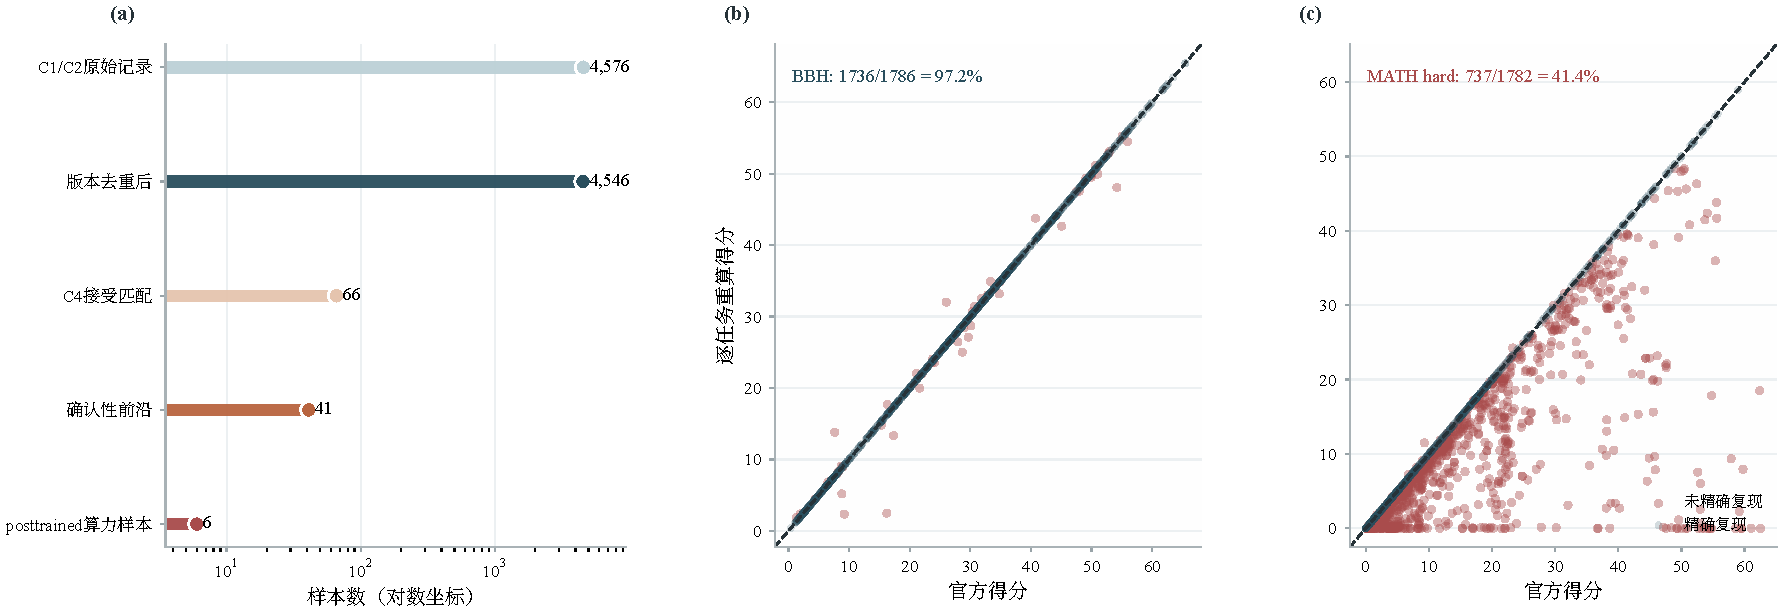
\includegraphics[width=0.98\textwidth]{images/no4/P4_F01_数据筛选与逐任务复现审计.pdf}
  \caption{问题四的数据筛选与逐任务复现审计}
  \label{fig:p4_data_audit}
\end{figure}

\subsubsection{综合能力与逐任务复现}

以六项官方归一化得分的算术均值定义模型 $i$ 的综合能力：
\begin{equation}
S_i^{\mathrm{avg}}=\frac{1}{6}\sum_{k=1}^{6}S_{ik},
\label{eq:p4_average_score}
\end{equation}
其中六项任务为 IFEval、BBH、MATH、GPQA、MUSR 和 MMLU-PRO。复算结果与官方 Average 的最大绝对误差为 $1.421\times10^{-14}$，说明量表闭合。为避免验证期信息泄漏，六维秩正态平衡分只作为敏感性指标，其经验分布函数始终在当期训练窗内估计。

根据 Open LLM Leaderboard 的官方归一化规则\cite{huggingface2024normalization}，BBH 的每个子任务须先扣除随机猜测下界，再对子任务等权平均。设模型 $i$ 在子任务 $j$ 上的原始分数为 $s_{ij}$，随机下界为 $l_j$，则
\begin{equation}
z_{ij}=\max\left\{0,\frac{s_{ij}-l_j}{1-l_j}\right\},\qquad
\widehat S_i^{\mathrm{BBH}}=\frac{100}{|J_i|}\sum_{j\in J_i}z_{ij}.
\label{eq:p4_bbh}
\end{equation}
在 $1786$ 个唯一可比模型中，重算 BBH 与官方分数精确一致的模型为 $1736$ 个，占 $97.2\%$，超过预注册的 $95\%$ 门槛。MATH hard 仅精确复现 $737/1782$，未达到门槛，故不作为正式逐任务复现证据。这一降级不会改变式~\eqref{eq:p4_average_score} 的官方综合能力主表。

\subsection{模型建立}

\subsubsection{Loss--Benchmark 单调桥接}

\subsubsection{有界变换与候选映射}

Loss 与下游能力虽总体负相关，但不同数据分布、模型族和离散任务转换会削弱这种关系；相同预训练 Loss 也可能对应不同的下游表现\cite{gadre2025scalereliably,liu2023samepretraining,schaeffer2025predicting,mayilvahanan2025line}。为保证能力预测自然落在 $0$--$100$，定义严格互逆的有界变换
\begin{equation}
g_{\epsilon}(S)=\operatorname{logit}\left(\frac{S+\epsilon}{100+2\epsilon}\right),\qquad
g_{\epsilon}^{-1}(y)=(100+2\epsilon)\sigma(y)-\epsilon,
\quad \epsilon=0.5,
\label{eq:p4_link}
\end{equation}
其中 $\sigma(\cdot)$ 为 Logistic 函数。该变换在 $0,5,50,99,100$ 五个校验点上的最大往返误差为 $1.421\times10^{-14}$。

对综合能力与六项任务分别拟合
\begin{equation}
g_{\epsilon}(S_{im})=h_m(\log L_i)+e_{im},
\qquad \frac{\mathrm d h_m(x)}{\mathrm dx}\le0,
\label{eq:p4_bridge}
\end{equation}
其中 $L_i$ 为验证 Loss，$h_m$ 为常数、单调线性、低自由度单调样条或保序回归之一。高可比记录权重为 $1$，中可比记录主权重为 $0.25$；按来源族留一验证计算 MAE、RMSE、Spearman 相关、区间覆盖率和区间宽度，并在最优 MAE 的一个标准误差内选择最简单模型。

Average 最终选择单调线性桥接，其 $12$ 个来源族折外 MAE 为 $10.217$、RMSE 为 $12.387$，优于常数基线 MAE $11.383$。IFEval、MATH 和 GPQA 未稳定优于常数基线，标记为弱桥接目标，不能承担综合能力主结论。完整桥接支持域为 Loss $1.65$--$2.84$，其中严格高可比范围为 $2.0933$--$2.5978$；范围外预测必须带外推标签，不作无标识延伸。

图~\ref{fig:p4_bridge_validation} 展示 one-SE 选模及留来源族验证结果，图~\ref{fig:p4_bridge_models} 则横向比较七类能力目标的候选桥接误差。二者共同支持“综合能力采用单调线性桥接、弱目标降级使用”的选择。

\begin{figure}[H]
  \centering
  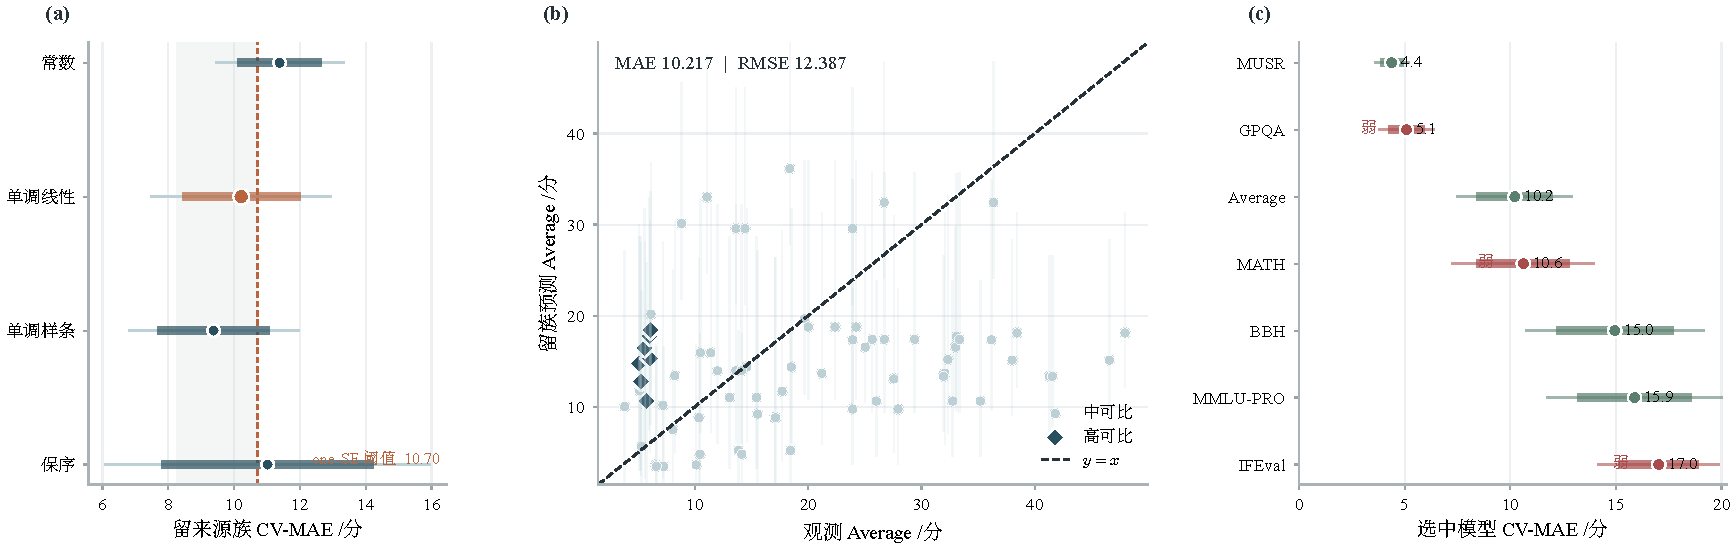
\includegraphics[width=0.99\textwidth]{images/no4/P4_F02_Loss_Benchmark桥接选择与留族验证.pdf}
  \caption{Loss--Benchmark 桥接的 one-SE 选模与留来源族验证}
  \label{fig:p4_bridge_validation}
\end{figure}

\begin{figure}[H]
  \centering
  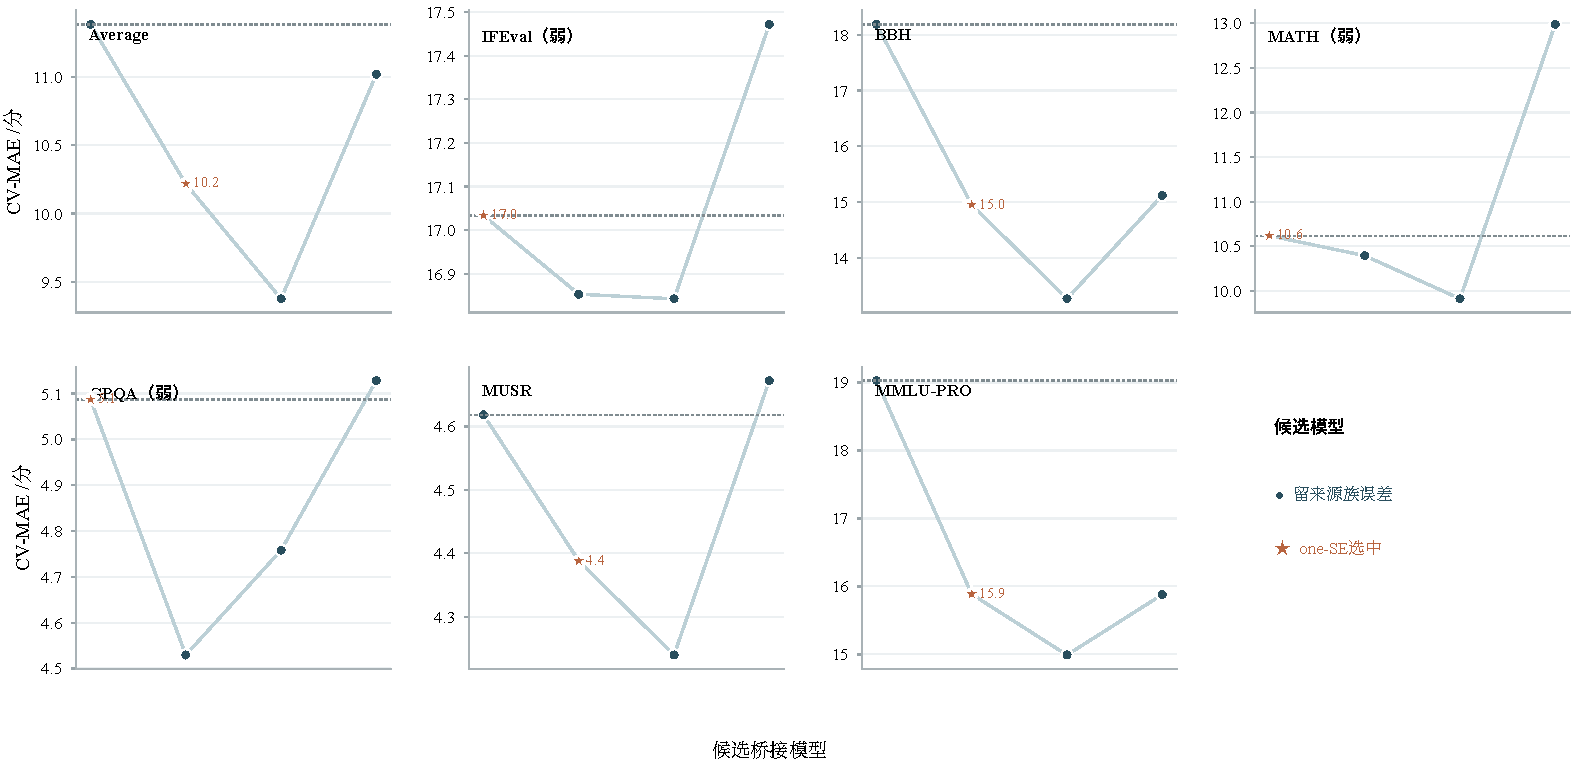
\includegraphics[width=0.97\textwidth]{images/no4/P4_A01_七类能力桥接模型比较.pdf}
  \caption{七类能力目标的候选桥接模型留来源族误差}
  \label{fig:p4_bridge_models}
\end{figure}

\subsubsection{问题三方案的能力映射}

问题三的每个 Loss bootstrap 样本与桥接来源族 bootstrap 配对传播，分别形成仅上游、仅桥接和联合三组区间。$45$ 个情景中，$15$ 个为高支持、$15$ 个为扩展支持、$15$ 个超出桥接范围。以正文主情景 $L_{\mathrm{ctx}}=4096$ 为例，三类质量成本下的综合能力映射见表~\ref{tab:p4_p3_mapping}。

图~\ref{fig:p4_p3_mapping} 先给出全部问题三方案从 Loss 到综合能力的连续映射，再由表~\ref{tab:p4_p3_mapping} 报告代表性预算点的数值和支持标签。图表并用可避免将范围外方案与高支持方案混为同等可信度。

\begin{figure}[H]
  \centering
  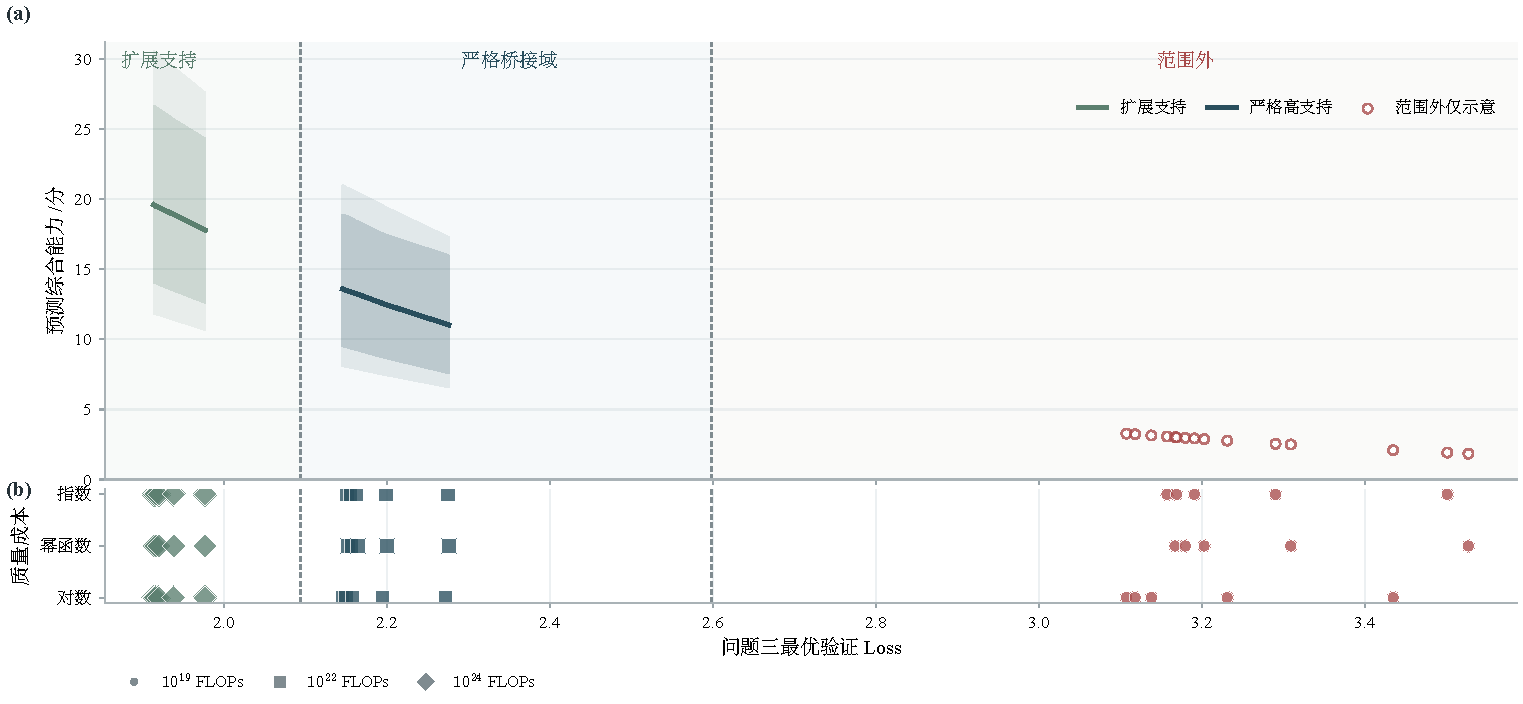
\includegraphics[width=0.98\textwidth]{images/no4/P4_F03_问题三Loss到综合能力映射.pdf}
  \caption{问题三最优 Loss 到综合能力的局部桥接映射}
  \label{fig:p4_p3_mapping}
\end{figure}

\begin{table}[htbp]
\centering
\caption{4096上下文下问题三最优Loss到综合能力的映射}
\label{tab:p4_p3_mapping}
\small
\setlength{\tabcolsep}{4.5pt}
\begin{tabular}{llrrrl}
\toprule
质量成本 & 预算/FLOPs & 最优 Loss & 能力中位数 & $80\%$ 区间 & 桥接支持 \\
\midrule
指数 & $10^{19}$ & $3.16898$ & $3.00$ & $[1.68,6.26]$ & 范围外，有限证据 \\
指数 & $10^{22}$ & $2.15491$ & $13.39$ & $[9.37,18.68]$ & 高支持 \\
指数 & $10^{24}$ & $1.91601$ & $19.51$ & $[14.02,26.56]$ & 扩展支持 \\
\midrule
幂函数 & $10^{19}$ & $3.17962$ & $2.97$ & $[1.63,6.24]$ & 范围外，有限证据 \\
幂函数 & $10^{22}$ & $2.15634$ & $13.36$ & $[9.35,18.63]$ & 高支持 \\
幂函数 & $10^{24}$ & $1.91611$ & $19.51$ & $[14.02,26.56]$ & 扩展支持 \\
\midrule
对数 & $10^{19}$ & $3.11805$ & $3.22$ & $[1.83,6.63]$ & 范围外，有限证据 \\
对数 & $10^{22}$ & $2.14975$ & $13.49$ & $[9.46,18.80]$ & 高支持 \\
对数 & $10^{24}$ & $1.91567$ & $19.52$ & $[14.03,26.57]$ & 扩展支持 \\
\bottomrule
\end{tabular}
\end{table}

表~\ref{tab:p4_p3_mapping} 表明，三种质量成本在中、高预算下映射出的综合能力非常接近，这是因为问题三的质量变量达到上界后，最优 Loss 主要由参数量和训练 Token 数决定。低预算方案的 Loss 高于 C6 完整支持上界，因此能力值仅用于回答题设情景，不能视为有直接观测支撑的精确预测。不确定性分解还显示，以指数成本、$10^{19}$ FLOPs 为例，上游 Loss 的 $80\%$ 映射宽度仅为 $0.078$ 分，而桥接不确定性宽度为 $4.687$ 分，说明结论的不确定性主要来自 Loss--Benchmark 映射而不是问题三优化器。

\subsection{模型求解}

\subsubsection{动力学能力前沿}

\subsubsection{条件分位模型}

能力前沿关注给定训练规模和时点下较优模型能够达到的水平，因此采用 $\tau=0.90$ 条件分位而非条件均值。分位回归能够直接刻画条件分布的高分位\cite{koenker1978quantiles}。令 $Y_i=g_{\epsilon}(S_i^{\mathrm{avg}})$，$x_i=\log_{10}C_i$，并将 $x_i$ 标准化为 $\widetilde x_i$，建立
\begin{equation}
Q_{\tau}(Y_i\mid x_i,t_i)
=\beta_0+\beta_C\widetilde x_i+a_{m(i)},
\qquad \beta_C\ge0,
\label{eq:p4_frontier}
\end{equation}
其中 $a_{m(i)}$ 为提交月份对应的非规模状态。主模型不同时放入 $C,N,D$，以避免 $C\approx6ND$ 引起机械共线；参数量模型 M-N 和参数--数据模型 M-ND 仅作机制诊断。

月度状态采用低自由度局部线性动力学
\begin{equation}
a_m=a_{m-1}+v_{m-1}+\eta_m,
\qquad
v_m=v_{m-1}+\zeta_m.
\label{eq:p4_state}
\end{equation}
数值实现用平滑 pinball 损失，并对状态的一阶与二阶差分施加惩罚。平滑强度 $\lambda$ 与未来状态斜率的局部权重 $\rho$ 只根据 $3$ 个月和 $6$ 个月滚动预测起点回测选择，保证每一折只使用预测时点以前的数据\cite{hyndman2021forecasting}。最终选得 $\lambda=10000$、$\rho=0$，即在当前短面板下采用高度平滑的状态并以全局斜率作保守外推；标准化算力系数 $\widehat\beta_C=0.6852>0$。

图~\ref{fig:p4_compute_frontier} 将确认性 pretrained 样本、平滑状态轨迹与算力方向置于同一坐标系中。该图的作用不是把相关性包装为因果性，而是直观核对：在控制观测期后，较高训练算力与较高动力学能力状态保持一致方向，且前沿外推没有脱离历史样本的局部支撑。

\begin{figure}[H]
  \centering
  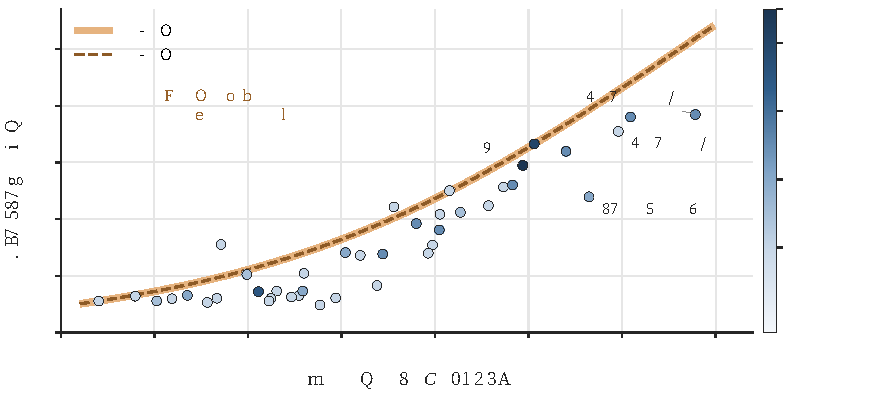
\includegraphics[width=0.94\textwidth]{images/no4/P4_F04_训练算力与动力学能力前沿.pdf}
  \caption{确认性 pretrained 样本的训练算力与动力学能力前沿}
  \label{fig:p4_compute_frontier}
\end{figure}


\subsubsection{求解与联合不确定性传播}

问题四从数据审计到前沿预测的完整计算过程归纳为算法~\ref{alg:p4_pipeline}。

\begin{algorithm}[H]
\caption{分层证据融合与动力学能力前沿预测}
\label{alg:p4_pipeline}
\begin{algorithmic}[1]
\Require C1--C6、C8，问题三冻结情景，分位集合 $\{0.85,0.90,0.95\}$，算力情景集合 $\{1,0.5,0.25\}$
\Ensure 综合能力、桥接结果、贡献分解与 $12/24$ 月前沿区间
\State 核验附件哈希、字段和子集关系，执行版本级去重与 C1/C2--C4 实体匹配
\State 按开放权重证据和模型类型构造确认性 pretrained 前沿面板
\State 由式~\eqref{eq:p4_average_score} 重建综合能力，并按式~\eqref{eq:p4_bbh} 复算 BBH
\ForAll{综合能力与六项任务目标}
    \State 对四类单调桥接执行来源族留一验证，并按一个标准误差规则选模
    \State 配对重采样问题三 Loss 与桥接来源族，输出支持域标签和能力区间
\EndFor
\State 滚动回测选择 $\lambda$ 与 $\rho$，拟合三条动力学分位前沿
\State 在模型家族簇与连续月份块上联合 bootstrap，并重估历史贡献
\State 按 C4 证据层构造月度算力前沿，在每次抽样中重估截止端点与增速
\ForAll{算力情景与预测时长}
    \State 预测三条分位前沿，对交叉分位执行单调重排并同步更新 link 与得分
\EndFor
\State 检查上游隔离、单调性、Shapley 闭合、分位次序、外推标签和复现性
\end{algorithmic}
\end{algorithm}

历史贡献的不确定性以模型家族为横截面簇、以连续月份为时间块进行重采样；未来预测还在每个抽样中重新估计算力端点、增长率和算力测量误差。时间相关数据采用块 bootstrap 的依据见文献\cite{kunsch1989bootstrap}。三条分位在每个抽样内部联合拟合，若发生交叉，则通过单调重排恢复 $q_{0.85}\le q_{0.90}\le q_{0.95}$\cite{chernozhukov2010quantile}，并由各自重排后的抽样计算区间。

\subsection{结果分析与模型验证}

\subsubsection{规模与非规模残余贡献}

选取确认性面板首末可用月份 $t_0=\text{2024-06}$、$t_1=\text{2025-01}$，并以各月训练算力的 $0.90$ 分位 $x_0,x_1$ 代表前沿规模。记 $F(x,t)$ 为式~\eqref{eq:p4_frontier} 经式~\eqref{eq:p4_link} 逆变换后的能力分。由于模型非线性，先替换规模和先替换时间会产生不同的边际增量，故采用两因素 Shapley 路径平均\cite{shapley1953value}：
\begin{align}
\Delta_{\mathrm{scale}}
&=\frac12\left\{F(x_1,t_0)-F(x_0,t_0)
+F(x_1,t_1)-F(x_0,t_1)\right\},\label{eq:p4_scale_contribution}\\
\Delta_{\mathrm{tech}}
&=\frac12\left\{F(x_0,t_1)-F(x_0,t_0)
+F(x_1,t_1)-F(x_1,t_0)\right\}.\label{eq:p4_tech_contribution}
\end{align}
两项必须满足
\begin{equation}
\Delta_{\mathrm{scale}}+\Delta_{\mathrm{tech}}
=F(x_1,t_1)-F(x_0,t_0).
\label{eq:p4_shapley_closure}
\end{equation}

分解结果见表~\ref{tab:p4_contribution}。中心估计的总变化为 $4.6182$ 分，其中规模扩张相关贡献为 $4.6183$ 分，非规模残余贡献为 $-0.0001$ 分。后者的 $80\%$ 区间跨越零，bootstrap 正号概率仅为 $0.528$，因此当前七个月现代面板不能识别稳定的非规模方向。本文不把接近零的中心残余解释为“技术没有进步”，而是认为在现有样本、口径和高度平滑的状态模型下，无法从规模项之外分离出稳定增量。

\begin{table}[htbp]
\centering
\caption{2024年6月至2025年1月的能力前沿贡献分解}
\label{tab:p4_contribution}
\small
\setlength{\tabcolsep}{8pt}
\begin{tabular}{lrrr}
\toprule
分解量 & 中心估计/分 & $80\%$ 区间/分 & $95\%$ 区间/分 \\
\midrule
能力总变化 & $4.6182$ & $[2.8418,5.6627]$ & $[2.5333,6.6860]$ \\
规模扩张相关贡献 & $4.6183$ & $[2.8407,5.6644]$ & $[2.5325,6.6868]$ \\
非规模残余贡献 & $-0.0001$ & $[-0.0018,0.0037]$ & $[-0.0027,0.0053]$ \\
\bottomrule
\end{tabular}
\end{table}


图~\ref{fig:p4_contribution_joint} 进一步给出两类贡献在联合不确定性下的分布。由于非规模项中心值略为负，普通百分比会出现符号反转或近零分母问题，故正文统一报告绝对贡献与绝对份额；规格与长期历史方向敏感性在本节末集中讨论。

\begin{figure}[H]
  \centering
  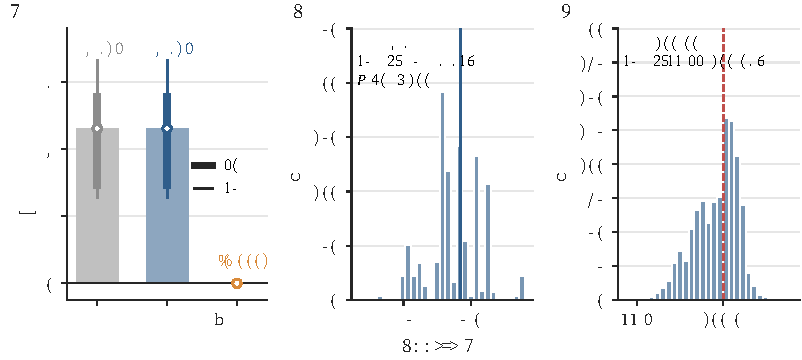
\includegraphics[width=0.80\textwidth]{images/no4/P4_F05_规模与非规模贡献联合分布.pdf}
  \caption{规模贡献与非规模残余贡献的联合分布}
  \label{fig:p4_contribution_joint}
\end{figure}

\subsubsection{算力放缓情景与未来能力前沿}

\subsubsection{算力端点与增长情景}

训练算力只使用预测截止日以前、开放权重、语言模型且证据方法为直接报告、运算计数或硬件估计的 C4 记录。算力估计的证据层、上下界和置信度处理遵循 Epoch AI 对训练算力估计方法的说明\cite{epoch2025computeestimation}；由 Benchmark 反推的算力不得再用于 Benchmark--算力关系，以避免循环论证。

同一家族同一月份先保留算力前沿版本，再在近 $24$ 个月的家族月面板上估计加权 $0.90$ 分位。稳健局部线性趋势给出截止月端点
\begin{equation}
x_{C,0}=25.092,\qquad
r_C=0.759\ \log_{10}(\mathrm{FLOPs})/\text{年},
\label{eq:p4_compute_growth}
\end{equation}
其中截止月原始月前沿为 $24.356$，最近三个月中位前沿为 $24.544$。端点使用截止月趋势拟合值而非全样本无时间条件分位，并在每个 bootstrap 抽样中与增速一同重估。

设算力增速保留系数 $\kappa\in\{1,0.5,0.25\}$，预测 $h$ 个月后的算力为
\begin{equation}
x_C(h;\kappa)=x_{C,0}+\kappa r_C\frac{h}{12}.
\label{eq:p4_compute_scenario}
\end{equation}
三种情景分别表示延续近期趋势、中度放缓和强度放缓。能力前沿由式~\eqref{eq:p4_frontier} 在未来月份的状态外推与式~\eqref{eq:p4_compute_scenario} 联合给出。

图~\ref{fig:p4_compute_scenarios} 将历史月度算力前沿与三条未来路径并列展示。本文缩放的是未来对数增长率，而不是把既有算力水平机械折减。

\begin{figure}[H]
  \centering
  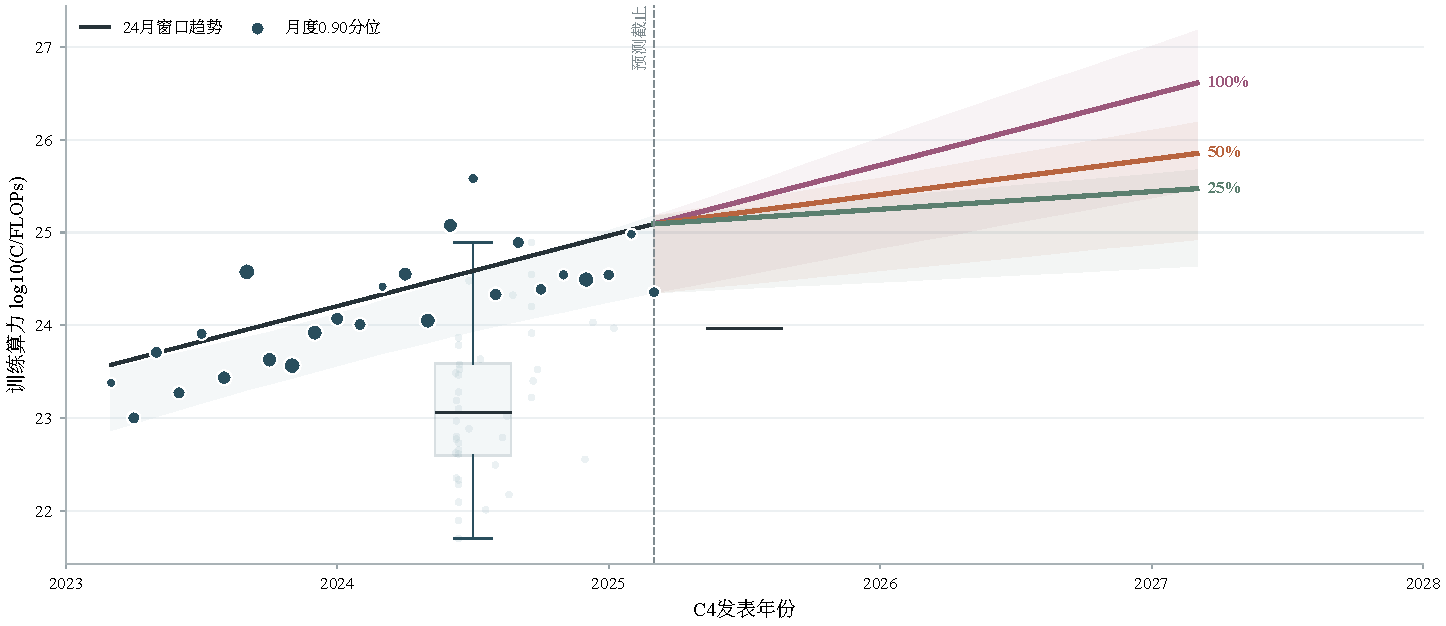
\includegraphics[width=0.98\textwidth]{images/no4/P4_F06_训练算力趋势与放缓情景.pdf}
  \caption{训练算力历史趋势与三种增长放缓情景}
  \label{fig:p4_compute_scenarios}
\end{figure}


\subsubsection{12个月与24个月预测}

主分位 $\tau=0.90$ 的结果见表~\ref{tab:p4_forecast}。全部区间同时包含历史前沿参数、未来状态斜率、算力端点、算力增速与算力测量误差；预注册 $1000$ 次联合抽样中获得 $999$ 次有效预测。

\begin{table}[htbp]
\centering
\caption{不同算力增速情景下的0.90能力前沿预测}
\label{tab:p4_forecast}
\small
\setlength{\tabcolsep}{6pt}
\begin{tabular}{lrrrr}
\toprule
算力情景 & 时长/月 & 前沿中心值 & $80\%$ 区间 & $95\%$ 区间 \\
\midrule
延续趋势（$\kappa=1$） & $12$ & $65.74$ & $[47.15,78.37]$ & $[40.25,86.09]$ \\
延续趋势（$\kappa=1$） & $24$ & $77.15$ & $[57.30,90.47]$ & $[47.49,95.29]$ \\
中度放缓（$\kappa=0.5$） & $12$ & $59.16$ & $[41.91,69.45]$ & $[36.47,77.85]$ \\
中度放缓（$\kappa=0.5$） & $24$ & $65.74$ & $[47.15,78.36]$ & $[40.25,86.08]$ \\
强度放缓（$\kappa=0.25$） & $12$ & $55.72$ & $[39.55,64.64]$ & $[34.60,72.52]$ \\
强度放缓（$\kappa=0.25$） & $24$ & $59.16$ & $[41.91,69.44]$ & $[36.47,77.85]$ \\
\bottomrule
\end{tabular}
\end{table}

图~\ref{fig:p4_future_frontier} 把表中六个点预测扩展为连续能力前沿。阴影区同时反映动力学状态、桥接模型和区组自助法的不确定性；放缓情景不仅压低中位前沿，也延后达到高能力区间的时间。

\begin{figure}[H]
  \centering
  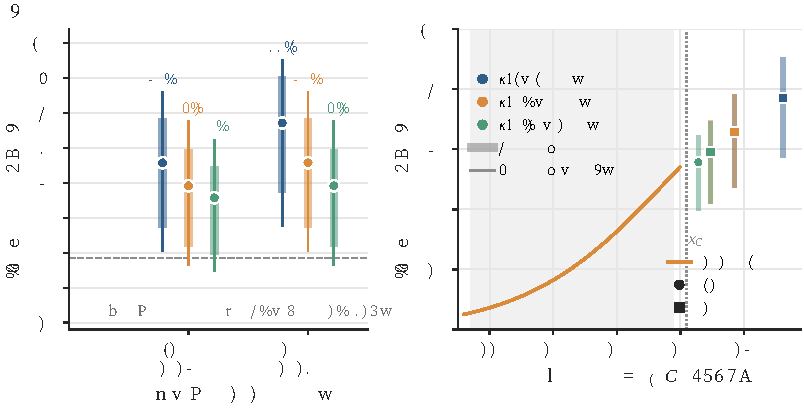
\includegraphics[width=0.96\textwidth]{images/no4/P4_F07_算力放缓下的未来能力前沿.pdf}
  \caption{算力增长放缓情景下的未来综合能力前沿}
  \label{fig:p4_future_frontier}
\end{figure}

预测结果具有清晰的情景递进性：算力增速越低、预测期越短，能力前沿越低；中度放缓 $24$ 个月与趋势延续 $12$ 个月的算力增量相同，因而前沿中心值均约为 $65.74$。然而，$12$ 个月结果已经超出同口径历史面板，必须标记为外推；$24$ 个月则属于长期外推。表中区间较宽，说明点预测不能脱离情景、区间和数据截止日单独使用。

\subsubsection{回测、数值验证与适用边界}

滚动起点回测在 $3$ 个月和 $6$ 个月步长上分别完成 $4$ 个有效起点。与 M-time 和 M-scale 基线比较，M-C 相对最佳基线 M-scale 的平均 pinball loss 差为 $0.00121$，配对标准误为 $0.00123$，未劣化超过一个标准误差，满足预注册放行条件。该回测只能检验短期排序和模型失效，不能被解释为对 $12/24$ 月外推的直接验证。

图~\ref{fig:p4_backtest_uncertainty} 同时呈现滚动回测误差和桥接区间宽度，避免仅用一条拟合曲线掩盖两类主要误差来源。近端回测支持方向稳定，但远端区间仍主要受外推距离和可迁移性假设支配。

\begin{figure}[H]
  \centering
  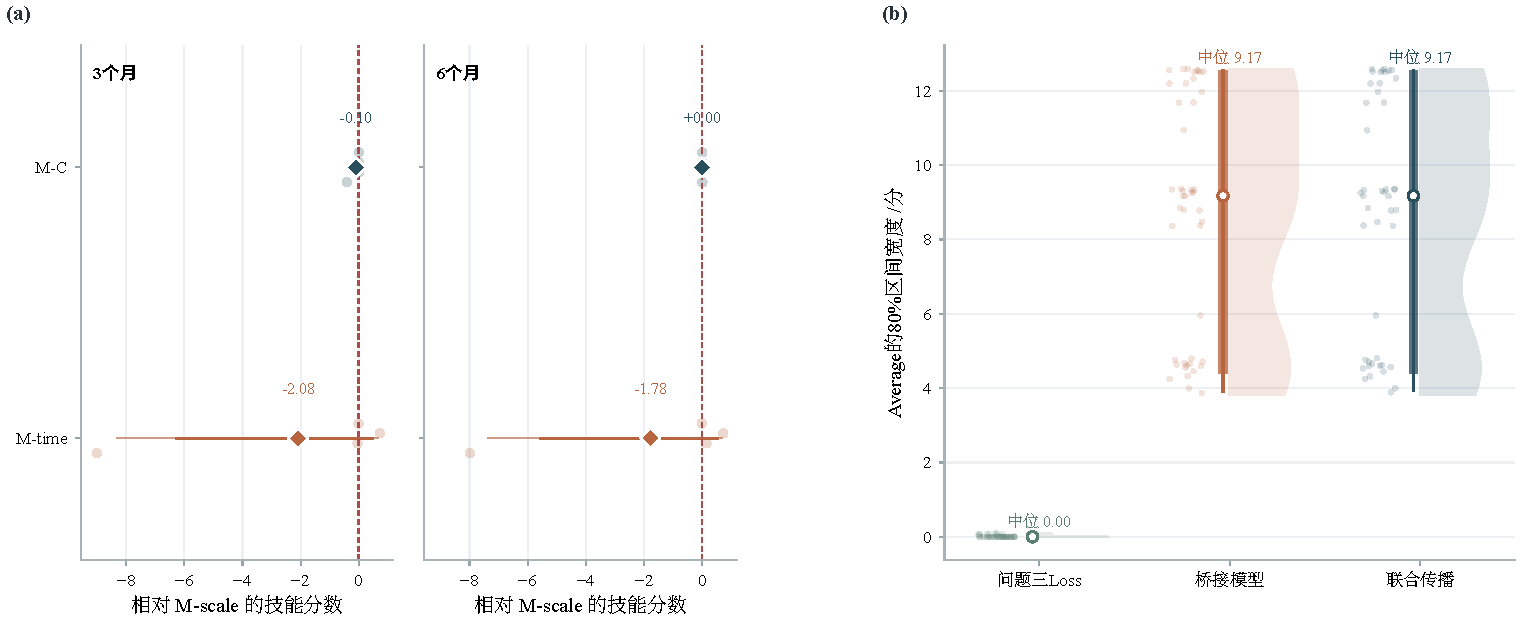
\includegraphics[width=0.96\textwidth]{images/no4/P4_F08_滚动回测与桥接不确定性.pdf}
  \caption{滚动回测误差与桥接不确定性诊断}
  \label{fig:p4_backtest_uncertainty}
\end{figure}


联合数值验收得到以下结果：全部桥接在稠密 Loss 网格上无单调违反；问题三 $45$ 个情景数量和标签保持不变，且进入历史训练集的数量为零；分数与 link 的最大不一致为零；三条分位在中心预测和抽样内均经重排保持有序；Shapley 在 link 与得分尺度的最大闭合误差为 $5.55\times10^{-17}$；相同配置连续运行两次的中心结果最大差为零。最终验收为 $29$ 项通过、$1$ 项警告、$0$ 项失败，数据、桥接、贡献分解、预测和总体五个接口均通过。唯一警告来自 MATH hard 逐任务重算未达到 $95\%$ 精确复现门槛，已通过只采用 BBH 正式证据完成降级处理。


\subsection{敏感性、适用边界与本问输出}

\subsubsection{贡献分解规格敏感性}

主口径采用严格 pretrained 样本、证据导向综合分数、发布时间轴、$\epsilon=1.5$ 和区组长度 3。分别改变样本边界、能力口径、时间轴、前沿容差与自助区组长度后，图~\ref{fig:p4_contribution_sensitivity} 中规模系数仍保持为正。不同设定会改变增量水平，但不改变“规模项主导、非规模残余缺乏稳定方向”的中心判断。

\begin{figure}[H]
  \centering
  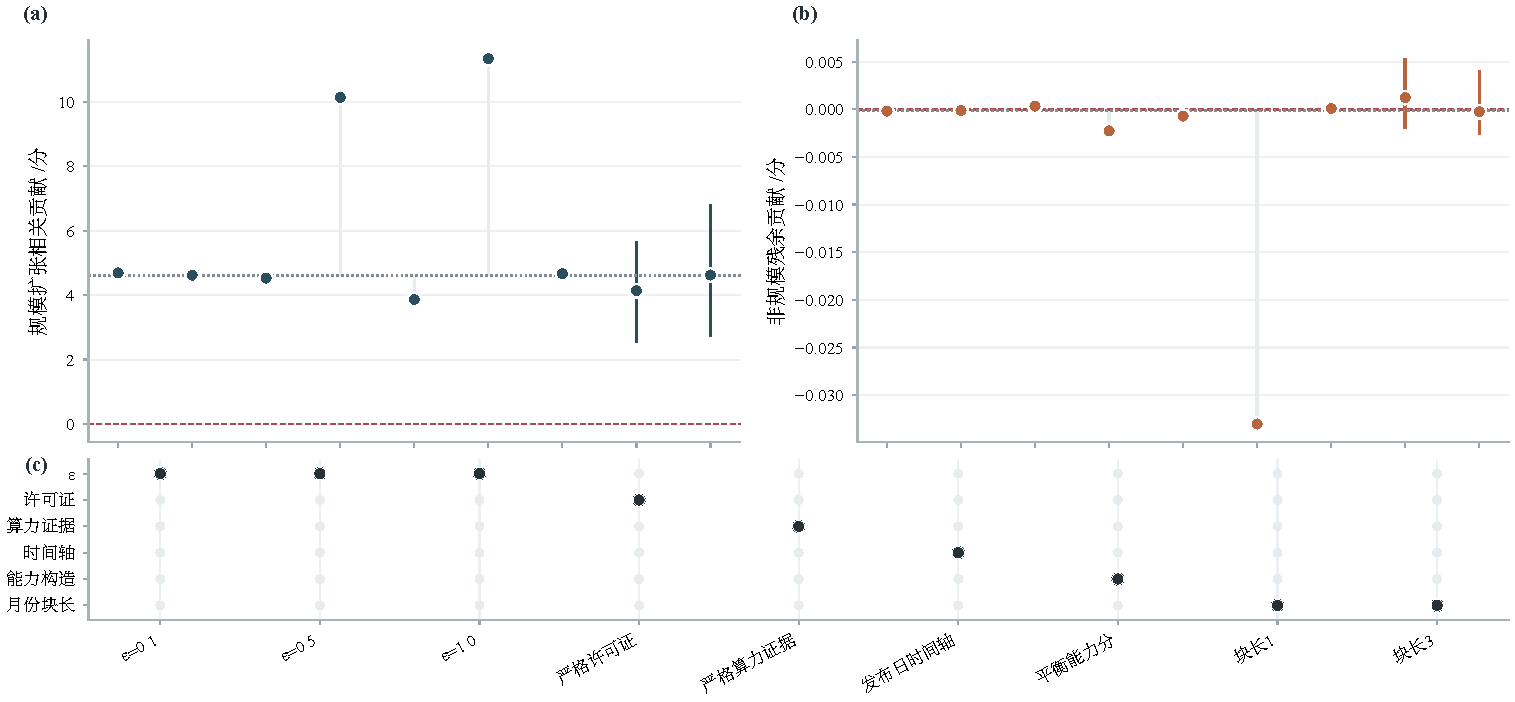
\includegraphics[width=0.98\textwidth]{images/no4/P4_A02_贡献分解规格敏感性.pdf}
  \caption{规模与非规模贡献分解的规格敏感性}
  \label{fig:p4_contribution_sensitivity}
\end{figure}

\subsubsection{长期历史方向敏感性}

2023--2024 年长期窗口仅包含 C3 与 C4 两个不同代际前沿点，因而只能承担方向核验。图~\ref{fig:p4_c3_sensitivity} 显示，引入 C3 历史信息没有推翻主样本的算力正向方向，但区间明显更宽、逐家族删除后符号不稳定，故不并入主估计。

\begin{figure}[H]
  \centering
  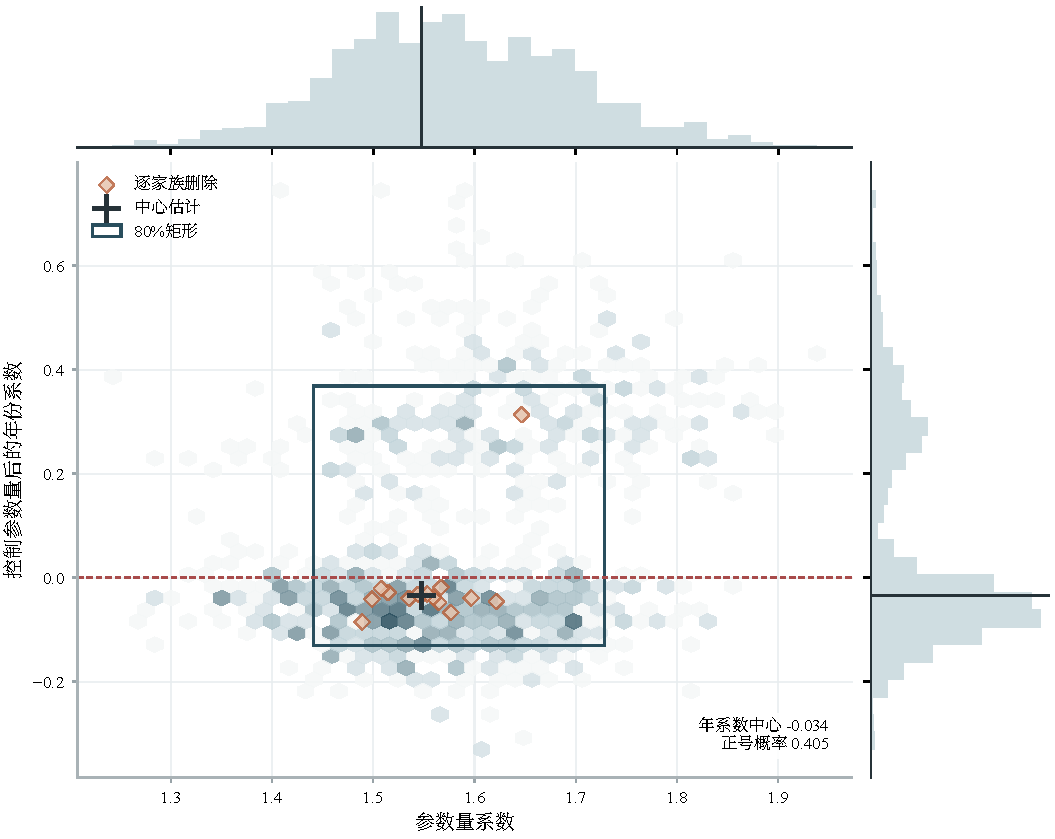
\includegraphics[width=0.80\textwidth]{images/no4/P4_A03_C3历史方向敏感性.pdf}
  \caption{引入 C3 历史信息后的方向敏感性}
  \label{fig:p4_c3_sensitivity}
\end{figure}

本问的适用边界有三点：第一，结论适用于公开可确认的 pretrained 前沿，不等同于对闭源训练过程的完全解释；第二，12/24 月结果是条件性情景预测，不是无条件点预测；第三，问题三样本只在训练后 Loss 的局部支撑域内用于桥接，域外情景仅用于风险提示。最终输出包括综合能力重建、算力--能力动力学前沿、规模与非规模贡献分解、三类算力放缓情景，以及相应的回测和敏感性证据。

综上，问题四在统一能力口径下完成了 Loss--Benchmark 映射、历史贡献分解与未来前沿预测。现有证据表明，2024 年 6 月至 2025 年 1 月的能力增量主要与训练规模扩张相关，控制规模后的非规模残余尚无稳定方向；若近期算力对数增速分别保留 $100\%$、$50\%$ 和 $25\%$，则 $24$ 个月后的 $0.90$ 能力前沿中心值约为 $77.15$、$65.74$ 和 $59.16$。这些结果是给定开放口径、数据截止日和算力情景下的条件预测，而不是确定性或因果性结论。


\section{模型的评价、改进与推广}

\subsection{模型优点}

本文的首要优点是将四个问题组织为可验收的分层证据链。问题一只在附件 A 内建立质量与配比响应，问题二只在附件 B 内估计绝对 Loss 标度律，跨体系信息通过 $Q_{\mathrm{ref}}$、$\boldsymbol p_{\mathrm{ref}}$ 和 $R(\boldsymbol p)$ 等显式接口传递，避免了将实验对象不同的 Loss 直接拼接。每一次向后传递都附带验收状态和适用边界，使“已识别的中心模型”与“仅用于敏感性的情景扩展”保持区分。

其次，各子模型均保留了对应的结构约束。质量评价对指标进行语义同向化并保留块间冲突；配比响应在单纯形上使用 Scheff\'e 混料结构；标度律对系数施加正值和单调性约束；资源配置同时考虑预算、质量上下界和观测支持域。问题三还利用目标对 $D$ 的单调性将三维优化解析降为二维，并以完整三维优化、加密网格和多起点轨迹交叉复核，降低了局部最优和单一初值造成的风险。

再次，模型不仅给出点估计，还通过分块交叉验证、外部对照、bootstrap、参数扰动和支持域标记报告不确定性。对于质量成本、质量尺度和长上下文等无法由当前附件唯一识别的要素，本文使用多情景比较而非将某一假设包装为确定事实，从而使结论的证据强度与表述强度相匹配。

\subsection{模型局限}

问题一中 $11$ 个推断域缺少与七个质量锚点等强的直接对齐证据，因而其领域质量回退到公共参考水平；这保证了稳健性，却牺牲了细粒度区分能力。配比响应面在 $1\mathrm{M}$、$60\mathrm{M}$ 和 $1\mathrm{B}$ 实测尺度上具有较好排序能力，但近优配比明显受支持半径、份额上界和局部解簇影响，不能直接解释为大模型训练中的唯一最优数据配方。

问题二的主要局限是跨体系可识别性。质量尺度只能以 $Q_{\mathrm{ref}}$ 为锚点作情景映射，配比响应 $R(\boldsymbol p)$ 则缺少映射到 B 体系绝对 Loss 的强度校准。因此，问题三必须固定 $\boldsymbol p_{\mathrm{ref}}$，并不能完整回答“配比与规模联合自由优化”的强形式问题。同时，高预算配置超出 B1/B7 的共同观测区间，三类质量成本又是题设情景而非实测工程成本，故问题三的高预算解应被视为条件外推。

问题四的确认性能力前沿样本只覆盖 $7$ 个月和 $13$ 个模型家族，非规模残余中还混合了数据工程、架构、优化和后训练等未充分观测因素。因此，当前贡献分解属于观察性分解，$12$ 个月与 $24$ 个月的预测属于带宽区间的情景外推，不应被解释为确定性或严格因果结论。

\subsection{改进方向}

最直接的改进是补充跨体系共同实验。可在同一模型族、同一验证集和统一训练流程下，对 $(N,D,Q_A,\boldsymbol p)$ 实施分层因子实验，为配比迁移强度 $\lambda_0$ 和质量尺度斜率 $s_Q$ 提供可识别数据。当共同实验覆盖充足时，可将固定配比优化扩展为配比、质量和规模的联合优化，并直接检验二阶交互是否随模型规模保持。

对资源配置模型，可进一步收集语料过滤、去重、合成、审核和存储的实际成本，将情景函数 $g(Q_A)$ 替换为经验成本曲线；同时把通信、内存、混合精度和硬件利用率纳入计算成本，将 FLOPs 约束扩展为多资源约束。对超出当前支持域的配置，应增加实际训练锚点或使用保守鲁棒优化，而不仅依赖幂律外推。

对能力前沿预测，应延长同口径时间面板，增加架构、数据处理、优化器、后训练算力和许可证等可比特征，并在更多历史起点上进行滚动回测。这将有助于把当前的“非规模残余”进一步拆分为更可解释的技术通道，并降低长期外推区间对短面板状态斜率的依赖。

\subsection{模型推广}

本文的分层框架不依赖某一特定大语言模型。对视觉基础模型、多模态模型或科学计算模型，只需把 Token 数替换为对应的样本、图像块或模态单元，重新定义质量信号和长序列成本，即可沿用“数据质量——性能标度——资源优化”的建模路径。在实际训练管理中，该框架也可作为情景规划工具：用可观测区间内的中心解给出基准配置，用质量成本、上下文和外推边界情景刻画决策风险，而不将单一点估计作为无条件的工程承诺。

\bibliographystyle{gmcm}
\bibliography{reference}


\end{document}
